\documentclass{mimosis}

\usepackage{metalogo}

%%%%%%%%%%%%%%%%%%%%%%%%%%%%%%%%%%%%%%%%%%%%%%%%%%%%%%%%%%%%%%%%%%%%%%%%
% Some of my favourite personal adjustments
%%%%%%%%%%%%%%%%%%%%%%%%%%%%%%%%%%%%%%%%%%%%%%%%%%%%%%%%%%%%%%%%%%%%%%%%
%
% These are the adjustments that I consider necessary for typesetting
% a nice thesis. However, they are *not* included in the template, as
% I do not want to force you to use them.

% This ensures that I am able to typeset bold font in table while still aligning the numbers
% correctly.
\usepackage{etoolbox}

\usepackage[binary-units=true]{siunitx}
\DeclareSIUnit\px{px}

\sisetup{%
  detect-all           = true,
  detect-family        = true,
  detect-mode          = true,
  detect-shape         = true,
  detect-weight        = true,
  detect-inline-weight = math,
}

%%%%%%%%%%%%%%%%%%%%%%%%%%%%%%%%%%%%%%%%%%%%%%%%%%%%%%%%%%%%%%%%%%%%%%%%
% Hyperlinks & bookmarks
%%%%%%%%%%%%%%%%%%%%%%%%%%%%%%%%%%%%%%%%%%%%%%%%%%%%%%%%%%%%%%%%%%%%%%%%

\usepackage[%
  colorlinks = true,
  citecolor  = RoyalBlue,
  linkcolor  = RoyalBlue,
  urlcolor   = RoyalBlue,
  ]{hyperref}

\usepackage{url}
\usepackage{nameref}
\usepackage[capitalise]{cleveref}



\usepackage{bookmark}

%%%%%%%%%%%%%%%%%%%%%%%%%%%%%%%%%%%%%%%%%%%%%%%%%%%%%%%%%%%%%%%%%%%%%%%%
% Bibliography
%%%%%%%%%%%%%%%%%%%%%%%%%%%%%%%%%%%%%%%%%%%%%%%%%%%%%%%%%%%%%%%%%%%%%%%%
%
% I like the bibliography to be extremely plain, showing only a numeric
% identifier and citing everything in simple brackets. The first names,
% if present, will be initialized. DOIs and URLs will be preserved.

\usepackage[%
  hyperref     = true,
  natbib       = true,
  sortcites    = true,
  maxbibnames  = 9,
  maxcitenames = 2,
  style        = numeric,
  ]{biblatex}

% %%%%%%%%%%%%%%%%%%%%%%%%%%%%%%%%%%%%%%%%%%%%%%%%%%%%%%%%%%%%%%%%%%%%%%%%
% Some adjustments to make the bibliography more clean
%%%%%%%%%%%%%%%%%%%%%%%%%%%%%%%%%%%%%%%%%%%%%%%%%%%%%%%%%%%%%%%%%%%%%%%%
%
% The subsequent commands do the following:
%  - Removing the month field from the bibliography
%  - Fixing the Oxford commma
%  - Suppress the "in" for journal articles
%  - Remove the parentheses of the year in an article
%  - Delimit volume and issue of an article by a colon ":" instead of
%    a dot ""
%  - Use commas to separate the location of publishers from their name
%  - Remove the abbreviation for technical reports
%  - Display the label of bibliographic entries without brackets in the
%    bibliography
%  - Ensure that DOIs are followed by a non-breakable space
%  - Use hair spaces between initials of authors
%  - Make the font size of citations smaller
%  - Fixing ordinal numbers (1st, 2nd, 3rd, and so) on by using
%    superscripts

% Remove the month field from the bibliography. It does not serve a good
% purpose, I guess. And often, it cannot be used because the journals
% have some crazy issue policies.
\AtEveryBibitem{\clearfield{month}}
\AtEveryCitekey{\clearfield{month}}

% Fixing the Oxford comma. Not sure whether this is the proper solution.
% More information is available under [1] and [2].
%
% [1] http://tex.stackexchange.com/questions/97712/biblatex-apa-style-is-missing-a-comma-in-the-references-why
% [2] http://tex.stackexchange.com/questions/44048/use-et-al-in-biblatex-custom-style
%
\AtBeginBibliography{%
  \renewcommand*{\finalnamedelim}{%
    \ifthenelse{\value{listcount} > 2}{%
      \addcomma
      \addspace
      \bibstring{and}%
    }{%
      \addspace
      \bibstring{and}%
    }
  }
}

% Suppress "in" for journal articles. This is unnecessary in my opinion
% because the journal title is typeset in italics anyway.
\renewbibmacro{in:}{%
  \ifentrytype{article}
  {%
  }%
  % else
  {%
    \printtext{\bibstring{in}\intitlepunct}%
  }%
}

% Remove the parentheses for the year in an article. This removes a lot
% of undesired parentheses in the bibliography, thereby improving the
% readability. Moreover, it makes the look of the bibliography more
% consistent.
\renewbibmacro*{issue+date}{%
  \setunit{\addcomma\space}
    \iffieldundef{issue}
      {\usebibmacro{date}}
      {\printfield{issue}%
       \setunit*{\addspace}%
       \usebibmacro{date}}%
  \newunit}

% Delimit the volume and the number of an article by a colon instead of
% by a dot, which I consider to be more readable.
\renewbibmacro*{volume+number+eid}{%
  \printfield{volume}%
  \setunit*{\addcolon}%
  \printfield{number}%
  \setunit{\addcomma\space}%
  \printfield{eid}%
}

% Do not use a colon for the publisher location. Instead, connect
% publisher, location, and date via commas.
\renewbibmacro*{publisher+location+date}{%
  \printlist{publisher}%
  \setunit*{\addcomma\space}%
  \printlist{location}%
  \setunit*{\addcomma\space}%
  \usebibmacro{date}%
  \newunit%
}

% Ditto for other entry types.
\renewbibmacro*{organization+location+date}{%
  \printlist{location}%
  \setunit*{\addcomma\space}%
  \printlist{organization}%
  \setunit*{\addcomma\space}%
  \usebibmacro{date}%
  \newunit%
}

% Do not abbreviate "technical report".
\DefineBibliographyStrings{english}{%
  techreport = {technical report},
}

% Display the label of a bibliographic entry in bare style, without any
% brackets. I like this more than the default.
%
% Note that this is *really* the proper and official way of doing this.
\DeclareFieldFormat{labelnumberwidth}{#1\adddot}

% Ensure that DOIs are followed by a non-breakable space.
\DeclareFieldFormat{doi}{%
  \mkbibacro{DOI}\addcolon\addnbspace
    \ifhyperref
      {\href{http://dx.doi.org/#1}{\nolinkurl{#1}}}
      %
      {\nolinkurl{#1}}
}

% Use proper hair spaces between initials as suggested by Bringhurst and
% others.
\renewcommand*\bibinitdelim {\addnbthinspace}
\renewcommand*\bibnamedelima{\addnbthinspace}
\renewcommand*\bibnamedelimb{\addnbthinspace}
\renewcommand*\bibnamedelimi{\addnbthinspace}

% Make the font size of citations smaller. Depending on your selected
% font, you might not need this.
\renewcommand*{\citesetup}{%
  \biburlsetup
  \small
}

\DeclareLanguageMapping{british}{bibliography-correct-ordinals}
\DeclareLanguageMapping{english}{bibliography-correct-ordinals}

% \bibliographystyle{ACM-Reference-Format}
\bibliography{Thesis}

%%%%%%%%%%%%%%%%%%%%%%%%%%%%%%%%%%%%%%%%%%%%%%%%%%%%%%%%%%%%%%%%%%%%%%%%
% Fonts
%%%%%%%%%%%%%%%%%%%%%%%%%%%%%%%%%%%%%%%%%%%%%%%%%%%%%%%%%%%%%%%%%%%%%%%%

\ifxetexorluatex
  \setmainfont{Minion Pro}
\else
  \usepackage[lf]{ebgaramond}
  \usepackage[oldstyle,scale=0.7]{sourcecodepro}
  \singlespacing
\fi

\renewcommand{\th}{\textsuperscript{\textup{th}}\xspace}

\newacronym[description={Principal component analysis}]{PCA}{PCA}{principal component analysis}
\newacronym                                            {SNF}{SNF}{Smith normal form}
\newacronym[description={Topological data analysis}]   {TDA}{TDA}{topological data analysis}

\newglossaryentry{LaTeX}{%
  name        = {\LaTeX},
  description = {A document preparation system},
  sort        = {LaTeX},
}

\newglossaryentry{Real numbers}{%
  name        = {$\real$},
  description = {The set of real numbers},
  sort        = {Real numbers},
}

\makeindex
\makeglossaries

% 12pt, please
% \KOMAoptions{fontsize=12pt}


% Basics
\usepackage{fixltx2e}
\usepackage{url}
\usepackage{fancyvrb}
\usepackage{mdwlist}  % Miscellaneous list-related commands

% https://www.nesono.com/?q=book/export/html/347
% Package for inserting TODO statements in nice colorful boxes - so that you
% won’t forget to fix/remove them. To add a todo statement, use something like
% \todo{Find better wording here}.
\usepackage{todonotes}

%% Math
\usepackage{bm}       % Bold symbols in maths mode
\usepackage{amssymb}

% http://tex.stackexchange.com/questions/114151/how-do-i-reference-in-appendix-a-theorem-given-in-the-body
\usepackage{thmtools, thm-restate}

%% Theoretical computer science
\usepackage{stmaryrd}
\usepackage{mathtools}  % For "::=" ( \Coloneqq )

%% Font
% \usepackage[euler-digits,euler-hat-accent]{eulervm}

\usepackage{pifont}

\usepackage{ottalt}

\usepackage{comment}

\usepackage{longtable}


% Code highlighting
\usepackage{listings}

\lstset{%
  % backgroundcolor=\color{white},
  basicstyle=\small\ttfamily,
  keywordstyle=\sffamily\bfseries,
  captionpos=none,
  columns=flexible,
  keepspaces=true,
  showspaces=false,               % show spaces adding particular underscores
  showstringspaces=false,         % underline spaces within strings
  showtabs=false,                 % show tabs within strings adding particular underscores
  breaklines=true,                % sets automatic line breaking
  breakatwhitespace=true,         % sets if automatic breaks should only happen at whitespace
  escapeinside={(*}{*)},
  literate={lam}{{$\lambda$}}1 {->}{{$\rightarrow$}}1 {Top}{{$\top$}}1 {o+o}{{$\oplus$}}1 {=>}{{$\Rightarrow$}}1 {and}{{$\land$}}1 {/\\}{{$\Lambda$}}1,
  tabsize=2,
  commentstyle=\color{purple}\ttfamily,
  stringstyle=\color{red}\ttfamily,
  sensitive=false
}

\lstdefinelanguage{sedel}{
  keywords={self, Void, Class, All, extends, this, trait, inherits, super, type, Trait, override, new, if, then, else, let, in, letrec},
  identifierstyle=\color{black},
  morecomment=[l]{--},
  morecomment=[l]{//},
  morestring=[b]",
  xleftmargin  = 3mm,
  morestring=[b]'
}


\lstdefinelanguage{simple}{
  keywords={letrec, in, let},
  identifierstyle=\color{black},
  xleftmargin  = 3mm,
}


\lstdefinelanguage{gbeta}{%
  language     = java,
  morekeywords = {virtual,refine},
  xleftmargin  = 3mm
}


\lstdefinelanguage{JavaScript}{
  keywords={function, const, extends, super, class, export, boolean, throw, implements, import, this, typeof, new, true, false, catch, function, return, null, catch, switch, var, if, in, while, do, else, case, break},
  identifierstyle=\color{black},
  comment=[l]{//},
  morecomment=[s]{/*}{*/},
  morestring=[b]',
  xleftmargin  = 3mm,
  morestring=[b]"
}


\lstset{language=sedel}

\theoremstyle{plain}
\newtheorem{theorem}{Theorem}
\newtheorem{lemma}{Lemma}
\newtheorem{corollary}{Corollary}
\newtheorem{proposition}{Proposition}
\theoremstyle{definition}
\newtheorem{definition}{Definition}
\newtheorem{example}{Example}
\newtheorem{observation}{Observation}
\theoremstyle{remark}
\newtheorem*{remark}{Remark}

% General
\newcommand{\code}[1]{\texttt {#1}}
\newcommand{\highlight}[1]{\colorbox{yellow}{#1}}

% Logic
\newcommand{\turns}{\vdash}

% PL
\newcommand{\subst}[2]{\lbrack #1 / #2 \rbrack}
\newcommand{\concatOp}{+\kern-1.3ex+\kern0.8ex}  % http://tex.stackexchange.com/a/4195/73122

% Constructors
\newcommand{\for}[2]{\forall #1. \, #2}
\newcommand{\lam}[2]{\lambda #1. \, #2}
\newcommand{\app}[2]{#1 \; #2}
\newcommand{\blam}[2]{\Lambda #1. #2}
\newcommand{\tapp}[2]{#1 \; #2}

\newcommand{\pair}[2]{\langle #1, #2 \rangle}
\newcommand{\inter}[2]{#1 \,\&\, #2}
\newcommand{\mer}[2]{#1 \, ,, \, #2}
\newcommand{\proj}[2]{{\code{proj}}_{#1} #2}
\newcommand{\ctx}[2]{#1\left\{#2\right\}}
\newcommand{\bra}[1]{\llbracket #1 \rrbracket}


\newcommand{\recordType}[2]{\{ #1 : #2 \}}
\newcommand{\recordCon}[2]{\{ #1 = #2 \}}

\newcommand{\ifThenElse}[3]{\code{if} \; #1 \; \code{then} \; #2 \; \code{else} \; #3}

\newcommand{\defeq}{\triangleq}

\newcommand{\logeq}[2]{#1 \backsimeq_{log} #2}
\newcommand{\kleq}[2]{#1 \backsimeq #2}
\newcommand{\ctxeq}[3]{#1 \backsimeq_{ctx} #2 : #3}

\newcommand{\stepn}{\longmapsto^*}
\newcommand{\step}{\longmapsto}


\newcommand{\name}{$\mathsf{NeColus}$\xspace}
\newcommand{\namee}{$\lambda_{i}^{+}$\xspace}
\newcommand\oname{$\lambda_{i}$\xspace}
\newcommand\fname{$\mathsf{F}_{i}$\xspace}
\newcommand\fnamee{$\mathsf{F}_{i}^{+}$\xspace}
\newcommand\tname{$\lambda_{co}$\xspace}
\newcommand\tnamee{$\mathsf{F}_{co}$\xspace}
\newcommand\sedel{$\mathsf{SEDEL}$\xspace}
\newcommand\visitor{\textsc{Visitor}s\xspace}

\newcommand{\cmark}{\ding{51}}%
\newcommand{\xmark}{\ding{55}}%



% Logical equivalence related macros
\newcommand{\valR}[2]{\mathcal{V}\bra{#1 ; #2}}
\newcommand{\valRR}[1]{\mathcal{V}\bra{#1}}
\newcommand{\eeR}[2]{\mathcal{E}\bra{#1 ; #2}}
\newcommand{\eeRR}[1]{\mathcal{E}\bra{#1}}
\newcommand{\ggR}[1]{\mathcal{G}\bra{#1}}
\newcommand{\ddR}[1]{\mathcal{D}\bra{#1}}

\newcommand{\hll}[2][gray!40]{\colorbox{#1}{#2}}
\newcommand{\hlmath}[2][gray!40]{%
  \colorbox{#1}{$\displaystyle#2$}}

\newcommand{\rulehl}[1]{}


% Ott includes
\inputott{ott-rules}
\renewcommand\ottaltinferrule[4]{
  \inferrule*[narrower=0.9,lab=#1,#2]
    {#3}
    {#4}
}

%%----------------------------------------------------------------------------%%
%%    Environment for Declaration                                             %%
%%----------------------------------------------------------------------------%%


\makeatletter
\newcommand{\makedeclaration}
{
\chapter*{Declaration}
% \addcontentsline{toc}{chapter}{Declaration}
\noindent I declare that this thesis represents my own work, except
where due acknowledgement is made, and that it has not been
previously included in a thesis, dissertation or report submitted
to this University or to any other institution for a degree,
diploma or other qualifications.
\vspace*{1.5in}

\noindent%
\begin{tabular}{@{}l@{}}
\dotfill \\
\@author\hspace*{3cm}\\
\@date\\
\end{tabular}
}

\makeatother

%%----------------------------------------------------------------------------%%
%%    Environment for Acknowledgments                                         %%
%%----------------------------------------------------------------------------%%

\makeatletter
\newcommand{\makeAck}
{
\chapter*{Acknowledgments}
% \addcontentsline{toc}{chapter}{Acknowledgements}

First and foremost, I would like to thank my PhD supervisor Dr. Bruno C. d. S.
Oliveira for his continued support and mentorship throughout my studies. I would
also like to thank my co-supervisor Prof. T.H. Tse for his valuable suggestions
and guidelines. He helped revise my papers and this thesis, continuously nudging
me to make my writing clearer. His feedback is nothing short of inspiring,
which I greatly enjoyed. Secondly, I would like to express my gratitude to Prof.
Tom Schrijvers from KU Leuven. I enjoyed very much our collaboration on a topic
of mutual interest, which lead to one of the key publications for this PhD
dissertation. I learned a lot from you! During the years I spent at HKU, I had
the opportunity to collaborate with a number of excellent fellow researchers, to
name a few, Tomas Tauber, Zhiyuan Shi, Weixin Zhang, Huang Li, Yanpeng Yang and
Ningning Xie. Last but not least, I would love to thank my family for being
extremely supportive throughout my studies. I made it through thanks to all of
you.
}
\makeatother


%%----------------------------------------------------------------------------%%
%%    Environment for Title Page                                              %%
%%----------------------------------------------------------------------------%%

\makeatletter
\renewcommand{\maketitle}
{%
  \begin{titlepage}
    \renewcommand{\baselinestretch}{1}
    \begin{center}
      \vspace*{\stretch{3}}
      {\LARGE\@title\par}
      \vspace*{1cm}
      {\large\textit{by}\par}
      \vspace*{1cm}
      {\Large\@author\par}
      \vspace*{\stretch{5}}
      {{
\includegraphics[width=30mm]{figures/hku}} \par}
      {\hbox{}\par}
      \vspace*{\stretch{5}}
      {
      	\textsl{(Temporary Binding for Examination Purposes)} \\
      	\vspace*{3cm}
      	{\normalsize
      	A thesis submitted in partial fulfillment of the requirements for \\
        the degree of Doctor of Philosophy \\
        at The University of Hong Kong \\
        \par
        }
      }
      \vspace*{\stretch{1}}
      {\large\@date\par}
      \vspace*{\stretch{1}}
    \end{center}
  \end{titlepage}
} \makeatother



%%%%%%%%%%%%%%%%%%%%%%%%%%%%%%%%%%%%%%%%%%%%%%%%%%%%%%%%%%%%%%%%%%%%%%%%
% Incipit
%%%%%%%%%%%%%%%%%%%%%%%%%%%%%%%%%%%%%%%%%%%%%%%%%%%%%%%%%%%%%%%%%%%%%%%%

\title{Disjoint Intersection Types: Theory and Practice}
\author{Xuan Bi}

\begin{document}

\frontmatter
  \maketitle
  % \begin{titlepage}
  \vspace*{5cm}
  \makeatletter
  \begin{center}
    \begin{Huge}
      \@title
    \end{Huge}\\[0.1cm]
    %
    \begin{Large}
      \@subtitle
    \end{Large}\\
    %
    \emph{by}\\
    \@author
    %
    \vfill
    A document submitted in partial fulfillment
    of the requirements for the degree of\\
    \emph{Doctor of Philosophy}\\
    at\\
    \textsc{The University of Hong Kong}
  \end{center}
  \makeatother
\end{titlepage}

\newpage
\null
\thispagestyle{empty}
\newpage

  \begin{center}
  \textsc{Abstract}
\end{center}
%
\noindent
%
Scientific documents often use \LaTeX{} for typesetting. While numerous
packages and templates exist, it makes sense to create a new one. Just
because.


  \makedeclaration
  \makeAck
  \tableofcontents
  \listoffigures
  \listoftables

\mainmatter

  
%%%%%%%%%%%%%%%%%%%%%%%%%%%%%%%%%%%%%%%%%%%%%%%%%%%%%%%%%%%%%%%%%%%%%%%%
\chapter{Introduction}
%%%%%%%%%%%%%%%%%%%%%%%%%%%%%%%%%%%%%%%%%%%%%%%%%%%%%%%%%%%%%%%%%%%%%%%%


% \begin{center}
%   \begin{minipage}{0.5\textwidth}
%     \begin{small}
%       In which the reasons for creating this package are laid bare for the
%       whole world to see and we encounter some usage guidelines.
%     \end{small}
%   \end{minipage}
%   \vspace{0.5cm}
% \end{center}


This thesis investigates the use of disjoint intersection types, a variant of
intersection types, focusing on its theoretical foundation and applications in
the context of Object-Oriented Programming. The results are three new typed
calculi, the first two being core calculi and the last one a source calculus,
combining the power of parametric polymorphism, a rich subtyping relation with
the fine-grained expressiveness of disjoint intersection types. The key
contribution of the thesis is that it unifies ideas that are seemingly unrelated
but powerful on their own in software engineering (nested composition, dynamic
inheritance, mixins, traits, extensible designs) by a single underlying
mechanism.


\section{(Disjoint) Intersection Types}


A central theme of this thesis is \textit{intersection types} (usually written $\inter{A}{B}$). Intersection
types~\citep{pottinger1980type, coppoInter} have a long history in
programming languages. They were originally introduced to characterize exactly
all strongly normalizing lambda terms. Since then, starting with
\citeauthor{reynolds1988preliminary}'s work on
Forsythe~\citep{reynolds1988preliminary}, they have also been employed to
express useful programming language constructs, such as key aspects of
\emph{multiple inheritance}~\citep{compagnoni1996higher} in Object-Oriented
Programming (OOP). One notable example is the Scala
language~\citep{odersky2004overview} and its DOT
calculus~\citep{amin2012dependent}, which make fundamental use of intersection
types to express a class/trait that extends multiple other traits. Other modern
languages, such as TypeScript~\citep{typescript}, Flow~\citep{flow} and
Ceylon~\citep{ceylon}, also adopt some form of intersection types.

Intersection types come in different varieties in the literature. Some calculi
provide an \emph{explicit} introduction form for intersections, called the
\emph{merge operator}. This operator was introduced by \citeauthor{reynolds1988preliminary} in Forsythe~\citep{reynolds1988preliminary} and
adopted by a few other calculi~\citep{Castagna_1992, dunfield2014elaborating, oliveira2016disjoint, alpuimdisjoint}. Unfortunately,
while the merge operator is powerful, it also makes it hard to get a \emph{coherent}
(or unambiguous) semantics.
%A semantics is said to be coherent if all valid programs have the
%same meaning.\tom{The previous sentence is easily misunderstood.}
Unrestricted uses of the merge operator can be ambiguous, leading to an incoherent semantics
where the same program can evaluate to different values.
%Perhaps because of this
%issue the merge operator has not been adopted by many language designs.
We shall come back to this form of intersection types in more details in
\cref{bg:sec:intersection}.

A far more common form of intersection types are the so-called \emph{refinement
  types}~\citep{Freeman_1991, Davies_2000, dunfield2003type}. Refinement types
restrict the formation of intersection types so that the two types in an
intersection are refinements of the same simple (unrefined) type. For example,
we can refine a type $\mathsf{Int}$ of integers with a subtype $\mathsf{Odd}$ of
odd numbers, then an integer $1$ can be typed as follows:
\[
  1 : \inter{\mathsf{Int}}{\mathsf{Odd}}
\]
which satisfies the restriction: both $\mathsf{Int}$ and $\mathsf{Odd}$ refine a
single simple type $\mathsf{Int}$. Refinement intersection increases only the
expressiveness of types (more precise properties can be checked) and not of
terms. For this reason, \citet{dunfield2014elaborating} argues that refinement
intersection is unsuited for encoding various useful language features that
require the merge operator (or an equivalent term-level operator).


Recently, \citet{oliveira2016disjoint} proposed \oname: a calculus with a variant of intersection types
called \emph{disjoint intersection types}.
Calculi with disjoint intersection types feature the merge
operator, with restrictions that all expressions in a merge
operator must have disjoint types and all well-formed intersections
are also disjoint. A bidirectional type system and the disjointness restrictions
ensure that the semantics of the resulting calculi remains
coherent.

Disjoint intersection types have great potential to serve as a foundation for
powerful, flexible and yet type-safe OO languages that are easy to reason about.
As shown by \citet{alpuimdisjoint}, calculi with disjoint intersection types are
very expressive and can be used to statically type-check JavaScript-style
programs using mixins. Yet they retain both type safety and coherence. While
coherence may seem at first of mostly theoretical relevance, it turns out to be
very relevant for OOP. Multiple inheritance is renowned for being tricky to get
right, largely because of the possible \emph{ambiguity} issues caused by the
same field/method names inherited from different parents~\citep{bracha1990mixin,
  scharli2003traits}. Disjoint intersection types enforce that the types of
parents are disjoint and thus that no conflicts exist. Any violations are
statically detected and can be manually resolved by the programmer (for example
by dropping one of the conflicting field/methods from one of the parents). This
is very similar to existing trait models~\citep{scharli2003traits,
  Ducasse_2006}. Therefore in an OO language modelled on top of disjoint
intersection types, coherence implies that no ambiguity arises from multiple
inheritance. This makes reasoning a lot simpler. As we will see, this thesis
realizes this vision by proposing a powerful OO language design that builds on
the idea of disjoint intersection types.

\section{Family Polymorphism}

One powerful and long-standing idea in OOP is \emph{family
  polymorphism}~\citep{Ernst_2001}. In family polymorphism inheritance is
extended to work on a \emph{whole family of classes}, rather than just a single
class. This enables high degrees of modularity and code reuse, enabling simple
solutions to hard programming language problems, like the Expression
Problem~\citep{wadler1998expression}. An essential feature of family
polymorphism is \emph{nested composition}~\citep{Corradi_2012, ErnstVirtual,
  Nystrom_2004}, which allows the automatic inheritance/composition of nested
(or inner) classes when the enclosing classes are composed. Designing a sound
type system that fully supports family polymorphism and nested composition is
notoriously hard; there are only a few, quite sophisticated, languages that
manage this~\citep{ErnstVirtual, Nystrom_2004, pubsdoc:tribe-virtual-calculus,
  SAITO_2007}. This thesis shows that the combination of the merge operator and
a rich subtyping relation captures the essence of nested composition.

%To make matters worse, combining
%multiple inheritance with family polymorphism requires dealing with the various
%issues of both ideas.


\section{First-Class Classes, Mixins and Traits}

Many dynamically-typed languages (including JavaScript, Ruby, Python or Racket)
support \emph{first-class classes}. In those languages classes are first-class
values and, like any other values, they can be passed as an argument, or
returned from a function. Furthermore first-class classes support \emph{dynamic
  inheritance}: i.e., they can inherit from other classes at \emph{runtime},
enabling programmers to abstract over the inheritance hierarchy. For example,
mixins~\citep{bracha1990mixin} become programmer-defined constructs -- a mixin is
simply a function that takes a class as an argument and returns a subclass. In
contrast, type system limitations prevent most statically-typed languages from
having first-class classes and dynamic inheritance.

Traits~\citep{scharli2003traits, Ducasse_2006} are an alternative to mixins, and
other models of (multiple) inheritance. The key difference between traits and
mixins lies on the treatment of conflicts when composing multiple traits/mixins.
Mixins adopt an \emph{implicit} resolution strategy for conflicts, where the
compiler automatically picks one implementation in case of conflicts. For
example, Scala uses the order of mixin composition to determine which
implementation to pick in case of conflicts. Traits, on the other hand, employ
an \emph{explicit} resolution strategy, where the compositions with conflicts
are rejected, and the conflicts are explicitly resolved by programmers.
\citet{scharli2003traits} make a good case for the advantages of the trait
model. In particular, traits avoid bugs that could arise from accidental
conflicts that were not noticed by programmers. With the mixin model, such
conflicts would be silently resolved, possibly resulting in unexpected runtime
behaviour due to a wrong method implementation choice. In a setting with dynamic
inheritance and first-class classes this problem is exacerbated by not knowing
all components being composed statically, greatly increasing the possibility of
accidental conflicts. From a modularity point-of-view, the trait model also
ensures that composition is \emph{commutative}, thus the order of composition is
irrelevant and does not affect the semantics. \citet{bracha1992programming}
claims that ``\emph{The only modular solution is to treat the name collisions as
  errors...}'', strengthening the case for the use of a trait model of
composition. Otherwise, if the semantics is affected by the order of
composition, global knowledge about the full inheritance graph is required to
determine which implementations are chosen. % \citet{scharli2003traits} discuss
% several other issues with mixins, which can be improved by traits. We refer to
% their paper for further details.
This thesis shows that with the merge operator
and disjoint intersection types, we are able to encode typed first-class traits.
Combined with the power of parametric polymorphism, we can further encode a very
dynamic form of mixin-style compositions, enabling highly modular designs with
Object Algebras~\citep{oliveira2012extensibility}.


\section{Contributions}

In this thesis, we present three new typed calculi, each building on top of the previous one.

\paragraph{The \namee Calculus.}

The first one named \namee is a simple calculus with records and disjoint
intersection types that supports \emph{nested composition}. The essential
novelty of \namee are distributivity rules between function/record types and
intersection types. These rules are the delta that enable extending the simple
forms of multiple inheritance/composition supported by \oname into a more
powerful form supporting nested composition. The key difficulty of adding
distributivity rules to a type system with disjoint intersection types is how to
preserve coherence. Although previous work on disjoint intersection types
proposes a solution to coherence, the solution imposes several ad-hoc
restrictions to guarantee the uniqueness of the elaboration and thus allow for a
simple syntactic proof of coherence. However such restrictions makes it hard or
impossible to adapt the proof to extensions of the calculus with distributivity
rules. To deal with coherence, we employ a more semantic proof method based on
\emph{logical relations}~\citep{tait, plotkin1973lambda, statman1985logical}.
Using the new proof method, we removed those restrictions and successfully
mechanized the coherence proof for \namee.

\paragraph{The \fnamee Calculus.}

The second one named \fnamee is a polymorphic calculus with disjoint
intersection types. \fnamee is essentially \namee enriched with a variant of
parametric polymorphic called disjoint polymorphism~\citep{alpuimdisjoint}. The
addition of parametric polymorphic increases the expressiveness power of \namee
dramatically, \fnamee is able to encode a very dynamic form of mixin-style
compositions. The first difficulty of adding parametric polymorphism is that
when a type variable occurs in an intersection type, it is not statically known
whether the instantiated type will be disjoint to other components of the
intersection (which may as well be type variables). The second difficulty is how
to prove coherence in the polymorphic setting. To address the first, \citet{alpuimdisjoint}
proposed \textit{disjointness constraint}, inspired by bounded
quantification~\citep{cardelli1994extension}, where type variables are constrained so that they are disjoint
to some given types. To address the second, we adapt the parametric logical
relation of System F to deal with disjoint polymorphism.



\paragraph{Typed First-Class Traits.}

Lastly we present the design of \sedel: a polymorphic (source) language with
\emph{first-class traits}, supporting \emph{dynamic inheritance} as well as
conventional OO features such as \emph{dynamic dispatching} and \emph{abstract
  methods}. Traits pose additional challenges when compared to models with
first-class classes or mixins, because method conflicts should be detected
\emph{statically}, even in the presence of features such as dynamic inheritance and
parametric polymorphism. To address the challenges of
typing first-class traits and detecting conflicts statically, \sedel adopts the
well-established approach of elaborating high-level language constructs to a
low-level core calculus. The main contribution of \sedel is to show how to model
source language constructs for first-class traits and dynamic inheritance. The
work on \namee and \fnamee aimed at core record calculi, and omits important
features for practical OO languages, including (dynamic) inheritance, dynamic
dispatching and abstract methods. Based on \citeauthor{cook1989denotational}'s
work on the denotational semantics for inheritance~\citep{cook1989denotational},
we show how to design a source language that is elaborated into \fnamee.
\sedel's elaboration into \fnamee is proved to be both type-safe and coherent.
Coherence ensures that the semantics of \sedel is unambiguous. In particular
this property is useful to ensure that programs using traits are free of
conflicts/ambiguities (even when the types of the object parts being composed
are not fully statically know). We illustrate the applicability of \sedel with
several example uses for first-class traits. Furthermore we conduct a case study
that modularizes programming language interpreters using a highly modular form
of \visitor.

In summary the contributions of this theis are:

\begin{itemize}

\item We present \namee, a calculus with disjoint intersection types that
  features both \emph{BCD-style subtyping} and \emph{the merge operator}. This
  calculus is both type-safe and coherent, and supports \emph{nested composition}.

\item We present \fnamee, a polymorphic calculus with disjoint intersection
  types. We show how \fnamee is able to provide basic support for dynamic mixins
  and basic operations of extensible records. \fnamee is both type-safe and
  coherent.

\item We present \sedel, a statically-typed language design that supports
  first-class traits, dynamic inheritance, as well as standard OO features such
  as dynamic dispatching and abstract methods. We show how the semantics of
  \sedel can be defined by elaboration into \fnamee.

\item A more flexible notion of disjoint intersection types where only merges
  need to be checked for disjointness. This removes the need for enforcing
  disjointness for all well-formed types, making type systems with disjoint
  intersections more easily extensible.

\item A more powerful proof strategy for coherence of type systems with disjoint
  intersection types based on logical relations.


\item A comprehensive Coq mechanization of all meta-theory. This has notably
  revealed several missing lemmas and oversights in Pierce's manual
  proof of BCD's algorithmic subtyping~\citep{pierce1989decision}. As a
  by-product, we obtain the first mechanically verified BCD-style subtyping
  algorithm with coercions.

\item A full-blown implementation of \sedel; it runs and type-checks all the
  examples in this thesis.\footnote{The Coq formalization and implementation are
    available at \url{https://goo.gl/R5hUAp}.} We also conduct a case study,
  which shows that support for composition of Object
  Algebras~\citep{oliveira2012extensibility} is greatly
  improved in \sedel. Using such improved design patterns we re-code the
  interpreters from an undergraduate textbook on programming
  languages~\citep{poplcook} in a modular way.

\end{itemize}


This thesis is largely based on two publications by the author, which are
indicated in the list below. The work on \fnamee is based on an on-going draft
by the author. In comparison to the original publications, this thesis contains
a more in-depth and consistent treatment of disjoint intersection types.

\begin{itemize}
\item Xuan Bi, Bruno C. d. S. Oliveira, and Tom Schrijvers. 2018. ``The Essence
  of Nested Composition''. In \textit{European Conference on Object-Oriented Programming (ECOOP)}.
\item Xuan Bi and Bruno C. d. S. Oliveira. 2018. ``Typed First-Class Traits''.
  In \textit{European Conference on Object-Oriented Programming (ECOOP)}.
\end{itemize}


The author also contributed to the following publications that do not directly
relate to the topics of this thesis:
\begin{itemize}
\item Ningning Xie, Xuan Bi, Bruno C. d. S. Oliveira. 2018. ``Consistent Subtyping for All''.
  In \textit{European Symposium on Programming (ESOP)}.
\item Yanpeng Yang, Xuan Bi, Bruno C. d. S. Oliveira. 2016. ``Unified Syntax with
  Iso-Types''. In \textit{Asian Symposium on Programming Languages and
    Systems (APLAS)}.
\item Tomas Tauber, Xuan Bi, Zhiyuan Shi, Weixin Zhang, Huang Li, Zhenrui Zhang,
  Bruno C. d. S. Oliveira. 2015. ``Memory-efficient Tail Calls in the JVM with
  Imperative Functional Objects''. In \textit{Asian Symposium on
    Programming Languages and Systems (APLAS)}.
\end{itemize}


\section{Structure of the Thesis}

The structure of the thesis is organized as follows:

\begin{description}
\item[Part I:] \Cref{chap:nested,chap:fi} formally define the type systems of
  \namee and \fnamee, respectively. We first give the syntax and semantics of
  the two calculi. The semantics is defined in two parts. The ``target''
  languages are two standard type systems (simply-typed $\lambda$-calculus and
  System F, respectively) that do not have intersection types, the merge
  operator or subtyping. The ``source'' languages, defined by translation into
  the target languages, contain intersection types, the merge operator and
  subtyping. We then prove some basic properties such as type safety of
  the elaboration, soundness and completeness of the algorithmic subtyping, etc.
\item[Part II:] \Cref{chap:coherence:simple,chap:coherence:poly} explore the
  issue of coherence. In \cref{chap:coherence:simple} we first propose a
  semantically-founded definition of coherence. We then use a proof method based
  on logical relations to establish coherence of \namee. In
  \cref{chap:coherence:poly} we follow the same technique in
  \cref{chap:coherence:simple} but encounter a severe issue of impredicativity. We
  then adapt the parametric logical relation and establish coherence of \fnamee.
\item[Part III:] In \cref{chap:traits} we present the syntax and semantics of
  \sedel. In particular we show how to elaborate source-level constructs for
  first-class traits into expressions of \fnamee. In \cref{chap:case_study} we
  conduct a case study of modularizing programming language features using a
  highly modular form of \visitor. Finally \cref{sec:related} reviews related
  work and \cref{chap:conclusion} presents some future work and concludes.
\end{description}

This thesis assumes familiarity with basic knowledge of programming languages
theory and object-oriented programming. We recommend
\citeauthor{DBLP:books/daglib/0005958}'s excellent textbook on programming
languages~\citep{DBLP:books/daglib/0005958} for a general introduction. In order
to keep this thesis as self-contained as possible, we begin with some
background in the main topics of this thesis, to set the stage for later
chapters.


%%% Local Variables:
%%% mode: latex
%%% TeX-master: "../Thesis"
%%% org-ref-default-bibliography: ../Thesis.bib
%%% End:

  
%%%%%%%%%%%%%%%%%%%%%%%%%%%%%%%%%%%%%%%%%%%%%%%%%%%%%%%%%%%%%%%%%%%%%%%%
\chapter{Background}
\label{chap:background}
%%%%%%%%%%%%%%%%%%%%%%%%%%%%%%%%%%%%%%%%%%%%%%%%%%%%%%%%%%%%%%%%%%%%%%%%

The chapter sets the stage for the three typed calculi that we are going to
present in later chapters by reviewing some relevant topics in this thesis. In
\cref{bg:sec:intersection} we start with the traditional formulation of
intersection types, followed by an introduction of the merge operator and the
issue of coherence. We then review the \oname calculus, the first calculus
featuring disjoint intersection types, and briefly discuss how disjointness
achieves coherence. In \cref{sec:ernst} we introduce family polymorphism by
means of presenting \citeauthor{ernst2004expression}'s elegant solution to the expression problem.
Finally in \cref{sec:bg:mixin:trait} we review the concepts of mixins and
traits, their drawbacks and strengths.




\section{Intersection Types}
\label{bg:sec:intersection}


Intersection types in the pure $\lambda$-calculus were developed in the late
1970s by \citet{coppoInter}, and independently by \citet{pottinger1980type}. The
original motivation to introduce intersection types was to devise a
type-assignment system \`a la Curry~\citep{CurryFeys} that satisfies the
following two properties:
\begin{enumerate}
\item The typing of a term should be preserved under $\beta$-conversion. (Under
  Curry's system, $\beta$-reduction preserves types but $\beta$-expansion, in
  general, does not.)
\item Every (strongly) normalizable term has a meaningful type. (We refer the
  reader to their paper for a precise definition of ``meaningful''.)
\end{enumerate}

The idea of intersection types is remarkably simple and natural. From the
set-theoretic perspective, an intersection type $[[A & B]]$ for every pair of
types $[[A]]$ and $[[B]]$ is thought of as containing all the elements of
$[[A]]$ that are also elements of $[[B]]$; from the type-theoretic point of
view, $[[A & B]]$ is a subtype of $[[A]]$, as well as of $[[B]]$; from the
order-theoretic point of view, $[[A & B]]$ is a greatest lower bound of $[[A]]$
and $[[B]]$~\footnote{Note that we say ``a'' rather than ``the'' because
  greatest lower bounds are not unique, but they are all ``equal'' to $[[A & B]]$
  in a sense that will be made more precise later.}. What may seem
surprising to OO programmers is that $[[A & B]]$ can also be viewed as a natural
analog of \textit{multiple inheritance}. If we read the subtyping $[[A <: B]]$
as ``$[[A]]$ is a subclass of $[[B]]$'', then $[[A & B]]$ is a name of a class
with all the common properties of $[[A]]$ and $[[B]]$. Of course, this analog is
not exact, in the same sense that inheritance is not
subtyping~\citep{cook1989inheritance}. But it is intuitively appealing, and as
we will see, can be made more precise in a sufficiently enriched calculus based
on intersection types.

Three subtyping rules capture the order-theoretic properties of intersection types:
\begin{mathpar}
  \inferrule*[lab=S-interL]{ }{ [[A & B <: A]] } \and
  \inferrule*[lab=S-interR]{ }{ [[A & B <: B]] } \and
  \inferrule*[lab=S-inter]{ [[C <: A]] \\ [[ C <: B  ]]  }{ [[C <: A & B ]] }
\end{mathpar}
Two nice consequences follow:
\begin{enumerate}
\item The top type $[[Top]]$ can be regarded as the 0-ary form of intersection. It is
  a maximum element of the subtyping ordering, i.e., $[[A <: Top]]$ for every
  type $[[A]]$.
\item Multiple-field record types can be thought of as an intersection of
  single-field record types. Thus, instead of
  \[
    [[ {  l1 : A1, ... , ln : An   }       ]]
  \]
  we can write
  \[
    [[ { l1 : A1} & ... & {ln : An} ]]
  \]
  Note that the width and depth subtyping rules of records become a
  consequence of the above subtyping rules of intersections.
\end{enumerate}

Two additional subtyping rules are usually found in the literature of
intersection types (e.g., see \citet{reynolds1988preliminary, Barendregt_1983}).
The first one captures the relation between intersections and function spaces,
allowing intersections to distribute over the right-hand side of $[[->]]$'s:
\[
    \inferrule*[lab=S-distArr]{ }{ [[(A1 -> A2) & (A1 -> A3) <: A1 -> A2 & A3]] }
\]
Note that the other direction is also derivable (cf. \cref{sec:typesystem}).
The second rule captures the relation between intersections and (singleton)
records, allowing intersections to distribute over record labels:
\[
    \inferrule*[lab=S-distRcd]{ }{ [[  { l : A } & { l : B } <: { l : A & B }   ]] }
\]

These two rules, though intuitively reasonable, will have a strong effect on both
syntactic and semantics properties of the language. For example, \rref{S-distArr} implies that
$[[ Top <: A -> Top ]]$ for any $[[A]]$; and \rref{S-distRcd} implies that $[[  Top <: {l : Top} ]]$.

The introduction form of intersection types says that a term $[[ee]]$ can be
given type $[[A & B]]$ if it inhabits both $[[A]]$ and
$[[B]]$:
\[
    \inferrule*[lab=T-interI]{ [[ee : A1]] \\  [[ee : A2]]   }{   [[ee : A1 & A2]]   }
\]
The corresponding elimination form allows us to derive, given a derivation of
$[[ ee : A1 & A2 ]]$, that $[[ee : A1]]$ and $ [[ee : A2]]$. But this already
follows from \rref{S-interL,S-interR} and the subsumption rule; so we need not
to add the elimination rule explicitly to the calculus.


\subsection{The Merge Operator}


Intersection types were first incorporated into a practical programming language
named Forsythe by \cite{reynolds1988preliminary, reynolds1997design}. who used
them to encode features such as operator overloading by means of a
``merge'' operator $p_1 ,, p_2$---``a construction for intersecting or
`merging' meanings''~\citep[p. 24]{reynolds1997design}.
(\citeauthor{reynolds1997design} actually used single comma $p_1 , p_2$,
but here we use double commas for consistency.) \citeauthor{reynolds1997design}
demonstrated the power of the merge operator by developing an encoding of
records by using intersection types; similar ideas also appear in
\citet{Castagna_1992}. The idea is to have only single-field records with the introduction form $[[ { l = e } ]]$ of type $[[ {l : A} ]]$ and
the usual eliminations (projection and pattern matching). Thus instead of
\[
  [[ {  l1 = ee1, ... , ln = een   }       ]]
\]
we can write
\[
  [[ { l1 = ee1} ,, ... ,, {ln = een} ]]
\]
which plays nicely with the syntactic sugar of multiple-field record types as
an intersection of single-field record types.

More recently, \citet{dunfield2014elaborating} developed a method for
elaborating intersections and unions into products and sums. Central to his
approach is a source-level \textit{merge operator} $[[ee1 ,, ee2]]$, reminiscent
of Forsythe~\citep{reynolds1997design}, which embodies several computationally
distinct terms, and can be checked against various parts of an intersection
type. In his system, the introduction form of intersection types is still
\rref{T-interI}, and two additional rules for the merge operator are added:
\begin{mathpar}
    \inferrule*[lab=T-mergeL]{ [[  ee1 : A  ]]   }{ [[  ee1 ,, ee2 : A   ]] } \and
    \inferrule*[lab=T-mergeR]{ [[  ee2 : A  ]]   }{ [[  ee1 ,, ee2 : A   ]] }
\end{mathpar}
In other words, a merge expression can choose to type one subterm and ignore the
other. In combination of \rref{T-interI}, they allow to type check
two distinct implementations $[[ee1]]$ and $[[ee2]]$ with completely different
types $[[A1]]$ and $[[A2]]$ of the intersection. For example, let $[[ee1]] = [[\x . x]]$ and $[[ee2]] = 1$,
then the type $[[ (nat -> nat) & nat ]]$ is inhabited by $[[ ee1 ,, ee2  ]]$:
\[
  \inferrule*[right=T-interI]
  { \inferrule*[right=T-mergeL]
    { [[ ee1 : nat -> nat  ]] }
    {[[ee1 ,, ee2 : nat -> nat]]}
    \\
    \inferrule*[right=T-mergeR]
    { [[ ee2 : nat  ]] }
    {[[ee1 ,, ee2 : nat]]}
  }
  { [[  ee1 ,, ee2 : (nat -> nat) & nat   ]] }
\]

\citeauthor{dunfield2014elaborating} then showed how to give a semantics to a
calculus with unrestricted intersection types by a type-directed elaboration to
a simply-typed $\lambda$-calculus extended with tuples. For example, the
expression $[[ (\x . x) ,, 1 ]]$ elaborates to a tuple $[[ <\x. x , 1> ]]$. As
usual, his system does not have explicit source-level intersection eliminations;
elaboration puts all needed projections into the target program. For example,
the same expression $[[ (\x . x) ,, 1 ]]$, when checked against $[[nat]]$, elaborates to $[[ pp2 <\x. x , 1> ]]$. The
type-directed elaboration is elegant, type-safe, and serves as the original
foundation for type systems with disjoint intersection types.


\subsection{Coherence}

While \citeauthor{dunfield2014elaborating}'s approach is simple and powerful, it
has serious usability issues. More specifically, it lacks the theoretically and
practically important property of \textit{coherence}~\citep{Reynolds_1991}: the
meaning of a target program depends on the choice of elaboration typing
derivation. For example, according to the elaboration rules, the expression $[[1
,, 2]]$ (when checked against $[[nat]]$) could elaborate to either $1$ or $2$,
depending on the particular choice in the implementation. The lack of coherence
is an important disadvantage for adopting his calculus in implementations of
programming languages. \citeauthor{dunfield2014elaborating} left it as an open
problem. To recover a coherent semantics, we could limit the merges according to
their surface syntax, as \citeauthor{reynolds1988preliminary} did in Forsythe.
But as \citet{dunfield2014elaborating} pointed out, ``crafting an
appropriate syntactic restriction depends on details of the type system, which
is not robust as the type system is extended''. The issue of coherence is later
addressed in an elegant way by \citet{oliveira2016disjoint} with the notion of
\textit{disjoint intersection types}.

\newcommand{\rulehl}[1]{#1}

\subsection{Disjoint Intersection Types}

\begin{figure}
  \centering
  \drules[Si]{$[[A <: B ~~> e]]$}{Subtyping}{int, top, arr, and, andL, andR}
  \drules[wf]{$[[GG |- A]]$}{Well-formedness of types}{int, top, and, arr}
  \drules[Ti]{$[[GG  |- ee => A ~~> e]]$}{Inference}{top, lit, var, app, anno, merge}
  \drules[Ti]{$[[GG  |- ee <= A ~~> e]]$}{Checking}{abs, sub}
  \caption{Type system of \oname}
  \label{fig:lambdai}
\end{figure}

Disjoint intersection types, first introduced in the \oname
calculus~\citep{oliveira2016disjoint} provide a remedy for the coherence
problem, by imposing restrictions on the uses of merges and on the formation of
intersection types. Its full type system is shown in \cref{fig:lambdai}. Central
to their approach is the notion of \textit{disjointness}. As a first
approximation, for two types $[[A]]$ and $[[B]]$ to be disjoint (written $[[A ** B]]$),
they must not have any sub-components sharing the same type. In a type
system without $[[Top]]$, this can be ensured by the following specification:

\begin{definition}[Simple disjointness] \label{def:disjoint_spec}
  $[[A ** B]] \defeq  \nexists C.\ [[A <: C]] \land [[B <: C]]$
\end{definition}

Disjointness judgment is used in the typing rule of merges (\rref{T-merge}) and
the well-formedness of intersection types (\rref{wf-and}). Now the expression
$[[1 ,, 2]]$ is not typable because $[[nat]]$ and $[[nat]]$ are not disjoint
(they have a common supertype $[[nat]]$). To ensure that subtyping produces
unique coercions, they also employ the notion of \textit{ordinary types}~\citep{Davies_2000}---those that are not intersection types---and
use the judgment ``$[[ A ord ]]$'' in \rref{Si-andL,Si-andR}. Ordinary types and
disjointness are sufficient to ensure a coherent semantics of a type system
without $[[Top]]$.

$[[Top]]$ brings extra complication, because \cref{def:disjoint_spec} does not
hold anymore ($[[Top]]$ is trivially a supertype of every type). To address this
problem, the notion of \textit{top-like types} were introduced, which are those
types that behave as $[[Top]]$ (such as $[[Top & Top]]$, $[[A -> Top]]$), and
captured by a predicate $ \rceil \cdot \lceil $. With top-types,
\cref{def:disjoint_spec} is refined to account for $[[Top]]$, as shown in
\cref{def:disjoint_spec2}. However, a careful analysis of
\cref{def:disjoint_spec2} shows that intersection types such as $[[ Top & Top
]]$ and $[[Top & nat]]$ are not well-formed because their constitute types are
not disjoint. This is one of the limitations in \oname, since ``a merge of two
$[[Top]]$-types will always return the same value regardless of which component
of the merge is chosen''~\citep{alpuimdisjoint}. In other words, $[[Top]]$ is
always disjoint to every other type. This restriction was later lifted by
\citet{alpuimdisjoint} in the \fname calculus by a set of inference rules, but
whether a corresponding specification of disjointness exists or not was not
known at that time. We will present a suitable specification in
\cref{sec:category}.

\begin{definition}[$[[Top]]$-Disjointness] \label{def:disjoint_spec2}
  $[[A ** B]] \defeq \neg \rceil [[A]] \lceil \ \land \ \neg \rceil [[B]] \lceil \ \land \
  (\forall C.\ [[A <: C]] \land [[B <: C]] \Longrightarrow \rceil [[C]] \lceil)$
\end{definition}

Combined with bidirectional type-checking, \citet{oliveira2016disjoint}
formalized the \oname calculus in Coq and prove that there is at most one
elaboration derivation for any expression, and as a consequence, there is only
one possible target program and thus coherence follows trivially. We refer the
reader to their paper for a detailed account of \oname.

In essence disjoint intersection types retain most of the expressive power of
the merge operator. For example, they can be used to model powerful forms of
extensible records~\citep{alpuimdisjoint}. However, forcing every intersection
types to be disjoint is unnecessarily restrictive. For instance,
$[[1 : nat & nat]]$ is undoubtedly unambiguous, but is rejected by \oname and \fname. Our
starting point in this thesis is to lift this restriction and makes room for
more expressiveness for calculi with disjoint intersection types.



\section{Family Polymorphism and Nested Composition}
\label{sec:ernst}
% %-------------------------------------------------------------------------------
% \subsection{Motivation: Family Polymorphism}

\emph{Family polymorphism} is the ability to simultaneously refine a family of
related classes through inheritance. This is motivated by a need to not only
refine individual classes, but also to preserve and refine their mutual
relationships. \citet{Nystrom_2004} call this \emph{scalable extensibility}:
``the ability to extend a body of code while writing new code proportional to
the differences in functionality''.
%
A well-studied mechanism to achieve family inheritance is \emph{nested
inheritance}~\citep{Nystrom_2004}. Nested inheritance combines two aspects.
Firstly, a class can have nested class members; the outer class is then a
family of (inner) classes. Secondly, when one family extends another, it
inherits (and can override) all the class members, as well as the relationships
within the family between the class members. However,
the members of the new family do not become subtypes of those in the parent family.

\paragraph{The Expression Problem}

\citet{ernst2004expression} illustrates the benefits of nested inheritance for modularity
and extensibility with one of the most elegant and concise solutions to the
\emph{Expression Problem}~\citep{wadler1998expression}. The expression problem,
as surveyed by \citet{togersen:2004}, is to answer the question:
\begin{quote}
  ``To which degree can your application be structured in such a way that both
  the data model and the set of virtual operations over it can be extended
  without the need to modify existing code, without the need for code repetition
  and without run-time type errors.''
\end{quote}
The expression problem is concerned with two-dimensional extensions:
\begin{inparaenum}[(1)]
\item adding new variants to the datatype;
\item and adding new operations on the datatype.
\end{inparaenum}
Depending on the programming style used in the code, it is usually
straightforward to add either new variants or new operations. For example, in an
OO language such as Java where an abstract datatype is represented by means of
classes whose methods are the operations on the datatype, it is easy to extend
the set of variants by writing another class. On the other hand, in a functional
language such as Haskell where the abstract datatype is modeled by means of
algebraic datatypes with a set of pattern matching functions as the operations,
then it is easy to add new operations by writing new pattern matching functions.
In either case, it is much harder to perform both extensions in the
\textit{same} language.


\paragraph{The Expression Problem, Scandinavian Style.}

Nowadays we know many solutions to the expression problem (for example, see
\citet{oliveira2012extensibility, wang2016expression, oliveira09modular,
  swierstra_2008, Zenger-Odersky2005}, to cite a few). Among all of them,
\citeauthor{ernst2004expression}'s solution is perhaps one of the most elegant
solutions out there. \citeauthor{ernst2004expression} solves the Expression
Problem in the \textsf{gbeta} language~\citep{ernst2000gbeta}, which he adorns with a Java-like syntax for
presentation purposes, for a small abstract syntax tree (AST) example. His
starting point is the code shown in \cref{fig:lang}. The outer class
\lstinline{Lang} contains a family of related AST classes: the common superclass
\lstinline{Exp} and two cases, \lstinline{Lit} for literals and \lstinline{Add}
for addition. The AST comes equipped with one operation, \lstinline{toString},
which is implemented by both cases. Notice that all the inner classes are
\textit{virtual}, in the same sense of virtual methods, which means that they
may be redefined in subclasses of the enclosing class.


\begin{figure}[t]
    \centering
    \begin{subfigure}[b]{0.45\textwidth}
\begin{lstlisting}[language=gbeta]
class Lang {
  virtual class Exp {
    String toString() {}
  }
  virtual class Lit extends Exp {
    int value;
    Lit(int value) {
      this.value = value;
    }
    String toString() {
      return value;
    }
  }
  virtual class Add extends Exp {
    Exp left,right;
    Add(Exp left, Exp right) {
      this.left = left;
      this.right = right;
    }
    String toString() {
      return left + "+" + right;
    }
  }
}
\end{lstlisting}
\subcaption{Base family: the language \lstinline{Lang}} \label{fig:lang}
    \end{subfigure} ~
    \begin{subfigure}[b]{0.5\textwidth}
\begin{lstlisting}[language=gbeta,  xleftmargin=1mm]
// Adding a new operation
class LangEval extends Lang {
  refine class Exp {
    int eval() {}
  }
  refine class Lit {
    int eval { return value; }
  }
  refine class Add {
    int eval { return
      left.eval() + right.eval();
    }
  }
}
// Adding a new case
class LangNeg extends Lang {
  virtual class Neg extends Exp {
    Neg(Exp exp) { this.exp = exp; }
    String toString() {
      return "-(" + exp + ")";
    }
    Exp exp;
  }
}
\end{lstlisting}
\subcaption{Extending in two dimensions} \label{fig:extend}
    \end{subfigure}
    \caption{The Expression Problem, Scandinavian Style}
\end{figure}

\paragraph{Adding a New Operation.}

One way to extend the family is to add an additional evaluation operation, as
shown in the top half of \cref{fig:extend}. This is done by subclassing the
\lstinline{Lang} class and refining all the contained classes by implementing
the additional \lstinline{eval} method. The semantics of the keyword
\lstinline[language=gbeta]{refine} is that the virtual class is constrained to
be a subclass of the new declaration. In other words, \lstinline{Exp},
\lstinline{Lit} and \lstinline{Add} are all extended with the \lstinline{eval}
method. Note that the inheritance between, e.g., \lstinline{Lang.Exp} and
\lstinline{Lang.Lit} is transferred to \lstinline{LangEval.Exp} and
\lstinline{LangEval.Lit}. Similarly, the \lstinline{Lang.Exp} type of the
\lstinline{left} and \lstinline{right} fields in \lstinline{Lang.Add} is
automatically refined to \lstinline{LangEval.Exp} in \lstinline{LangEval.Add}.

\paragraph{Adding a New Case.}

A second dimension to extend the family is to add a case for negation, shown in
the bottom half of \cref{fig:extend}. This is similarly achieved by subclassing
\lstinline{Lang}, and now adding a new contained virtual class \lstinline{Neg}
that represents the unary negation operator. Note that \lstinline{Neg} is
declared to be a subclass of \lstinline{Exp}, which means that the extension to
\lstinline{Exp} will also be added to \lstinline{Neg}.


\paragraph{Combining Both Extensions.}

Finally, the two extensions are naturally combined by means of
multiple inheritance, closing the diamond.
\begin{lstlisting}[language=gbeta]
class LangNegEval extends LangEval & LangNeg {
  refine class Neg {
    int eval() { return -exp.eval(); }
  }
}
\end{lstlisting}
The only effort required is to implement the one missing operation
case, evaluation of negated expressions.


\section{Mixins and Traits}
\label{sec:bg:mixin:trait}


Programmers have long realized that single inheritance is not flexible enough
when it comes to structuring a class hierarchy. For example, consider two
classes in different branches of the inheritance hierarchy, and assume that they
share features not inherited from their (unique) common parent. Attempting to
share the implementation of the common features may lead to putting the common
methods \textit{too high} in the hierarchy (i.e., they are forced into their
common parent), and these methods will be inherited by other classes in the same
hierarchy, which may not be desirable. On the other hand, putting those methods
in a \textit{lower} position results in code duplication. To overcome this
limitation, \textit{multiple inheritance} was proposed as a generalization of
single inheritance. However, as \citet{cook:multi} put it:
\begin{quote}
  ``Multiple inheritance is good, but there is no good way to do it.''
\end{quote}
One of the problems in multiple inheritance is the ambiguity issue that arises
when conflicting features are inherited along different paths. A classic
situation is the \emph{diamond problem}~\citep{bracha1990mixin} where a class
inherits from two parent classes that have a common superclass, as depicted by
\cref{fig:diamond}.


\begin{figure}
  \centering
  \begin{subfigure}[b]{0.45\textwidth}
    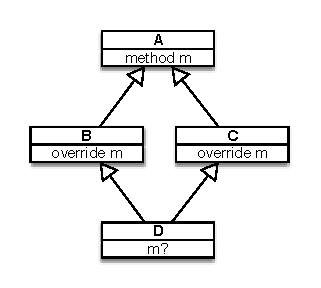
\includegraphics{figures/diamond.eps}
    \subcaption{The diamond problem} \label{fig:diamond}
  \end{subfigure} ~
  \begin{subfigure}[b]{0.45\textwidth}
    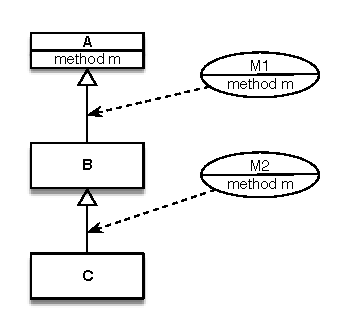
\includegraphics{figures/mixin.eps}
    \subcaption{Mixin composition} \label{fig:mixin}
  \end{subfigure}
  \caption{Multiple inheritance and mixins}
\end{figure}


Mixins and traits are two well-studied mechanisms to provide some form of
multiple inheritance. Mixins~\citep{bracha1990mixin} provide a simple mechanism
for multiple inheritance without the ambiguity issue. A mixin is a subclass
declaration parameterized over a superclass. Or simply put, a mixin can be
treated as a function from classes to classes. Thus the same mixin can be used to
extend a variety of parent classes with the same set of features.
\Cref{fig:mixin} shows a typical class hierarchy when using mixins. In the mixin
model, a class can inherit from another class by means of single inheritance as
usual. Apart from that, it can also have several mixins applied \textit{one at a
  time}. Let us take a close look at \cref{fig:mixin}. Both mixins
\lstinline{M1} and \lstinline{M2} contain a method \lstinline{m}, a question
arises as to which one is inherited in the class \lstinline{C}. The answer is
\lstinline{m} from the mixin \lstinline{M2}. This is because mixin composition
is \textit{linear}: methods defined in mixins appearing later override all the
identically named methods of earlier mixins. While this simple mechanism does
avoid conflicts, it also lead to other problems. For example, though we can
obtain the method \lstinline{m} from the mixin \lstinline{M1} by switching the
order of \lstinline{M1} and \lstinline{M2}, no suitable order of composition
exists to obtain \lstinline{m} from the superclass \lstinline{A}.

In respondence to the problems in the then compositional models,
\citet{scharli2003traits} proposed a mechanism called \textit{traits} as a
better way to foster code reuse in object-oriented programs. A trait is
essentially \textit{a set of pure methods}, divorced from any class hierarchy. A
trait \textit{provides} a set of methods to implement the behavior, and it may
also specify a set of \textit{required methods} that parameterize the provided
behavior. \Cref{fig:trait} shows a simple trait \lstinline{TCircle}, which
provides two methods \lstinline{hash} and \lstinline{area}, and requires a
method \lstinline{radius}. A class is then constructed by inheriting from a
superclass and incorporating a collection of traits, as shown in
\cref{fig:trait:conflict}. Also notice that there is a conflicting method
\lstinline{hash} that is provided by both \lstinline{TCircle} and
\lstinline{TDraw}. This is where the trait model is very different from the
mixin model. Unlike mixins that force a linear order in their composition,
traits can be composed in arbitrary order, and as a consequence, conflicting
methods must be resolved \textit{explicitly}, either by overriding the
conflicting methods, or by excluding a method from all but one trait.
\citet{scharli2003traits} discuss several other issues with mixins, which can be
improved by traits. We refer to their paper for a detailed account of traits.


\begin{figure}
  \centering
  \begin{subfigure}[b]{0.45\textwidth}
    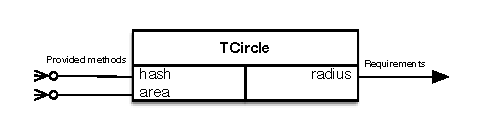
\includegraphics[scale=0.85]{figures/trait1.eps}
    \subcaption{A simple trait} \label{fig:trait}
  \end{subfigure} ~
  \begin{subfigure}[b]{0.45\textwidth}
    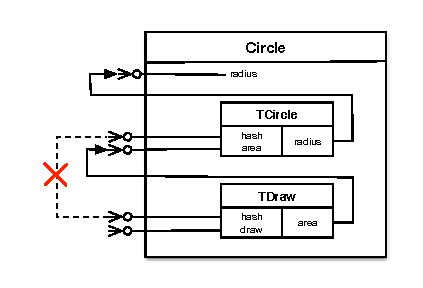
\includegraphics{figures/trait3.eps}
    \subcaption{Trait composition with conflicts} \label{fig:trait:conflict}
  \end{subfigure}
  \caption{Traits and conflicts}
\end{figure}

%%% Local Variables:
%%% mode: latex
%%% TeX-master: "../Thesis"
%%% org-ref-default-bibliography: ../Thesis.bib
%%% End:



  \part{Type Systems}

  
%%%%%%%%%%%%%%%%%%%%%%%%%%%%%%%%%%%%%%%%%%%%%%%%%%%%%%%%%%%%%%%%%%%%%%%%
\chapter{Semantics of the \namee Calculus}
\label{chap:nested}
%%%%%%%%%%%%%%%%%%%%%%%%%%%%%%%%%%%%%%%%%%%%%%%%%%%%%%%%%%%%%%%%%%%%%%%%

This chapter presents \namee, a calculus with disjoint intersection types that
features both BCD-style subtyping and the merge operator, which we believe
capture the essence of nested composition. We illustrate this by showing a neat
solution to the Expression Problem based on family polymorphism. We then discuss
the algorithmic aspects of \namee. The coherence property of \namee is discussed
in \cref{chap:coherence:simple}.

\section{Introduction}

\namee is a simple calculus with records and disjoint intersection types that
supports \emph{nested composition}. Nested composition enables encoding simple
forms of family polymorphism. More complex forms of family polymorphism,
involving binary methods~\citep{bruce1995binary} and mutable state are not yet
supported, but are interesting avenues for future work. Nevertheless, in \namee,
it is possible, for example, to encode Ernst's elegant family-polymorphism
solution~\citep{Ernst_2001} to the Expression Problem (cf.
\cref{nested:sec:overview}). Compared to \oname the essential novelty of
\namee are distributivity rules between function/record types and intersection
types. These rules are the delta that enable extending the simple forms of
multiple inheritance/composition supported by \oname into a more powerful form
supporting nested composition. The distributivity rule between function types
and intersections is common in calculi with intersection types aimed at
capturing the set of all strongly normalizable terms, and was first proposed by
\citet{Barendregt_1983} (BCD). However the distributivity rule is not common in
calculi or languages with intersection types aimed at programming. For example
the rules employed in languages that support intersection types (such as Scala,
TypeScript, Flow or Ceylon) lack distributivity rules. Moreover distributivity
is also missing from several calculi with a merge operator. This includes all
calculi with disjoint intersection types~\citep{oliveira2016disjoint,
  alpuimdisjoint} and \citeauthor{dunfield2014elaborating}'s work on elaborating
intersection types~\citep{dunfield2014elaborating}, which was the original
foundation for \oname. A possible reason for this omission in the past is that
distributivity adds substantial complexity (both algorithmically and
meta-theoretically), without having any obvious practical applications. This
thesis shows how to deal with the complications of BCD subtyping, while
identifying a major reason to include it in a programming language: BCD enables
nested composition and subtyping, which is of significant practical interest.

%The distributivity rules for records are
%new. Moreover, as far as we know, no previous work
%establishes the relation between BCD-style subtyping and nested composition.

\namee differs significantly from previous BCD-based calculi in that it has to
deal with the possibility of incoherence, introduced by the merge operator. Incoherence
is a non-issue in the previous BCD-based calculi because they do not feature
this merge operator or any other source of incoherence.
Although previous work on disjoint intersection types
proposes a solution to coherence, the solution imposes several ad-hoc restrictions
to guarantee the uniqueness of the elaboration and thus allow for a simple
syntactic proof of coherence (cf. \cref{sec:comparision}). Most
importantly, it makes it hard or impossible to adapt the proof to extensions of
the calculus, such as the new subtyping rules required by the BCD system.

In \namee we remove the brittleness of the previous syntactic method to prove
coherence, by employing a more semantic proof method based on \emph{logical
  relations}~\citep{tait, plotkin1973lambda, statman1985logical}. This new proof method has several
advantages. Firstly, with the new proof method, several restrictions that were
enforced by \oname to enable the syntactic proof method are removed. For example
the work on \oname has to carefully distinguish between so-called \emph{top-like
  types} and other types.
%This is necessary because top-like types can be
%non-disjoint (unlike other types), and yet they need to be allowed in a calculus
%with top types.
In \namee this distinction is not necessary; top-like types are handled like all
other types. Secondly, the method based on logical relations is more powerful
because it is based on semantic rather than syntactic equality. Finally, the
removal of the ad-hoc side-conditions makes adding new extensions, such as
support for BCD-style subtyping, easier. In order to deal with the complexity of
the elaboration semantics of \namee, we employ binary logical relations that are
heterogeneous, parameterized by two types; the fundamental property is also
reformulated to account for bidirectional type-checking.



\section{\namee by Examples}
\label{nested:sec:overview}

This section illustrates \namee with an encoding of a family polymorphism
solution to the expression problem, and informally presents its salient
features.


%-------------------------------------------------------------------------------
\subsection{The Expression Problem, \namee Style}

The \namee calculus allows us to solve the expression problem in a way that is
very similar to \citeauthor{Ernst_2001}'s \textsf{gbeta} solution in \cref{sec:ernst}.
However, the underlying mechanisms of \namee are quite different from those of
\textsf{gbeta}. In particular, \namee features a structural type system in which we can
model objects with records, and object types with record types. For instance, we
model the interface of \lstinline{Lang.Exp} with the singleton record type
\lstinline${ print : String }$. For the sake of conciseness, we use \lstinline{type} aliases
to abbreviate types.
\lstinputlisting[linerange=4-4]{./examples/overview.sl}% APPLY:linerange=PRINT_INTERFACE
Similarly, we capture the interface of the \lstinline{Lang} family in a record,
with one field for each case's constructor.
\lstinputlisting[linerange=8-8]{./examples/overview.sl}% APPLY:linerange=LANG_FAMILY
Here is the implementation of \lstinline{Lang}.
\lstinputlisting[linerange=17-24]{./examples/overview.sl}% APPLY:linerange=LANG_IMPL
We assume several primitive types: fixed width integers \lstinline{Int},
\lstinline{Double} for numeric operations and \lstinline{String} for text
manipulation. A \namee program consists of a collection of definitions and
declarations, separated by semicolon \lstinline{;}.

% - - - - - - - - - - - - - - - - - - - - - - - - - - - - - - - - - - - - - - - -
\paragraph{Adding evaluation.}
We obtain \lstinline{IPrint & IEval}, which is the corresponding type for \lstinline{LangEval.Exp}, by
intersecting \lstinline{IPrint} with \lstinline{IEval} where
\lstinputlisting[linerange=29-29]{./examples/overview.sl}% APPLY:linerange=EVAL_INTERFACE
The type for \lstinline{LangEval} is then
\lstinputlisting[linerange=34-37]{./examples/overview.sl}% APPLY:linerange=EVAL_PRINT_INTERFACE
We obtain an implementation for \lstinline{LangEval} by merging the existing
\lstinline{Lang} implementation \lstinline{implLang} with the new evaluation
functionality \lstinline{implEval} using the merge operator \lstinline{,,}.
\lstinputlisting[linerange=45-53]{./examples/overview.sl}% APPLY:linerange=EVAL_PRINT_IMPL

% - - - - - - - - - - - - - - - - - - - - - - - - - - - - - - - - - - - - - - - -
\paragraph{Adding negation.}
Adding negation to \lstinline{Lang} works similarly.
\lstinputlisting[linerange=57-65]{./examples/overview.sl}% APPLY:linerange=LANG_NEG
% \begin{Verbatim}[xleftmargin=10mm,fontsize=\relscale{.80}]
% type LangNeg = Lang & { neg : IPrint -> IPrint }

% implLangNeg : LangNeg
% implLangNeg = implLang ,, implNeg

% implNeg = { neg = \a.{print = "-" ++ a.print } }
% \end{Verbatim}

% - - - - - - - - - - - - - - - - - - - - - - - - - - - - - - - - - - - - - - - -
\paragraph{Putting everything together.}
Finally, we can combine the two extensions and provide the missing
implementation of evaluation for the negation case.
\lstinputlisting[linerange=70-80]{./examples/overview.sl}% APPLY:linerange=LANG_FINAL
We can test \lstinline{implLangNegEval} by creating an object that represents $-2 + 3$, which is able to print and evaluate at the same time.
\lstinputlisting[linerange=98-100]{./examples/overview.sl}% APPLY:linerange=TEST



%- - - - - - - - - - - - - - - - - - - - - - - - - - - - - - - - - - - - - - - -
\paragraph{Multi-field records.}
Recall that in \cref{bg:sec:intersection}, we show how to model multi-field records by
single-field records. Thus \namee does not have multi-field record types built in.
They are merely syntactic sugar for intersections of single-field record types.
Hence, the following is an equivalent definition of \lstinline{Lang}:
\lstinputlisting[linerange=13-13]{./examples/overview.sl}% APPLY:linerange=LANG_FAMILY2
Similarly, the multi-field record expression in the definition of
\lstinline{implLang} is syntactic sugar for the explicit merge of two
single-field records.
\begin{lstlisting}
implLang : Lang = { lit = ... } ,, { add = ... };
\end{lstlisting}

%- - - - - - - - - - - - - - - - - - - - - - - - - - - - - - - - - - - - - - - -
\paragraph{Subtyping.}
A distinctive difference compared to \textsf{gbeta} is that many more \namee types are related through
subtyping. Indeed, \textsf{gbeta} is unnecessarily conservative~\citep{ernst_hoh}: none of the families is related
through subtyping, nor is any of the class members of one family related to any
of the class members in another family. For instance, \lstinline{LangEval} is
not a subtype of \lstinline{Lang}, nor is \lstinline{LangNeg.Lit} a subtype
of \lstinline{Lang.Lit}.

In contrast, subtyping in \namee is much more nuanced and depends entirely on the
structure of types. The primary source of subtyping are intersection types:
any intersection type is a subtype of its components. For instance, 
\lstinline{IPrint & IEval} is a subtype of both \lstinline{IPrint} and
\lstinline{IEval}. Similarly \lstinline{LangNeg = Lang & NegPrint} is a subtype
of \lstinline{Lang}. Compare this to \textsf{gbeta} where \lstinline{LangEval.Expr} is
not a subtype of \lstinline{Lang.Expr}, nor is the family \lstinline{LangNeg} a
subtype of the family \lstinline{Lang}.

However, \textsf{gbeta} and \namee agree that \lstinline{LangEval} is not a subtype of
\lstinline{Lang}. The \namee-side of this may seem contradictory at first, as we
have seen that intersection types arise from the use of the merge operator.
We have created an implementation for \lstinline{LangEval} with
\lstinline{implLang ,, implEval} where \lstinline{implLang} has type \lstinline{Lang}, which
suggests that \lstinline{LangEval} is a subtype of \lstinline{Lang}.
Yet, there is a flaw in our reasoning:
strictly speaking, \lstinline{implLang ,, implEval} is not of
type \lstinline{LangEval} but instead of type \lstinline{Lang & EvalExt}, where
\lstinline{EvalExt} is the type of \lstinline{implEval}:
\lstinputlisting[linerange=41-41]{./examples/overview.sl}% APPLY:linerange=EVAL_INTERFACE2

Nevertheless, the definition of \lstinline{implLangEval} is valid because
\lstinline{Lang & EvalExt} is a subtype of \lstinline{LangEval}.
Indeed, if we consider for the sake of simplicity only the \lstinline{lit}
field, we have that \lstinline{(Int -> IPrint) & (Int -> IEval)} is a
subtype of \lstinline{Int -> IPrint & IEval}. This follows from a standard
subtyping axiom for distributivity of functions and intersections in the BCD system inherited by \namee.
In conclusion, \lstinline{Lang & EvalExt} is a subtype of both \lstinline{Lang}
and of \lstinline{LangEval}. However, neither of the latter two types is a subtype of the other.
Indeed, \lstinline{LangEval} is not a subtype of \lstinline{Lang} as the type
of \lstinline{add} is not covariantly refined and thus admitting the subtyping
is unsound. For the same reason \lstinline{Lang} is not a subtype of \lstinline{LangEval}.


A summary of the various relationships between the language components is shown
in \cref{fig:diagram}. Admittedly, the figure looks quite complex because our
calculus has a structural type system (as often more foundational calculi
do) where more types are related through subtyping, whereas mainstream object-oriented
languages have nominal type systems.



\begin{figure}[t]
  \centering
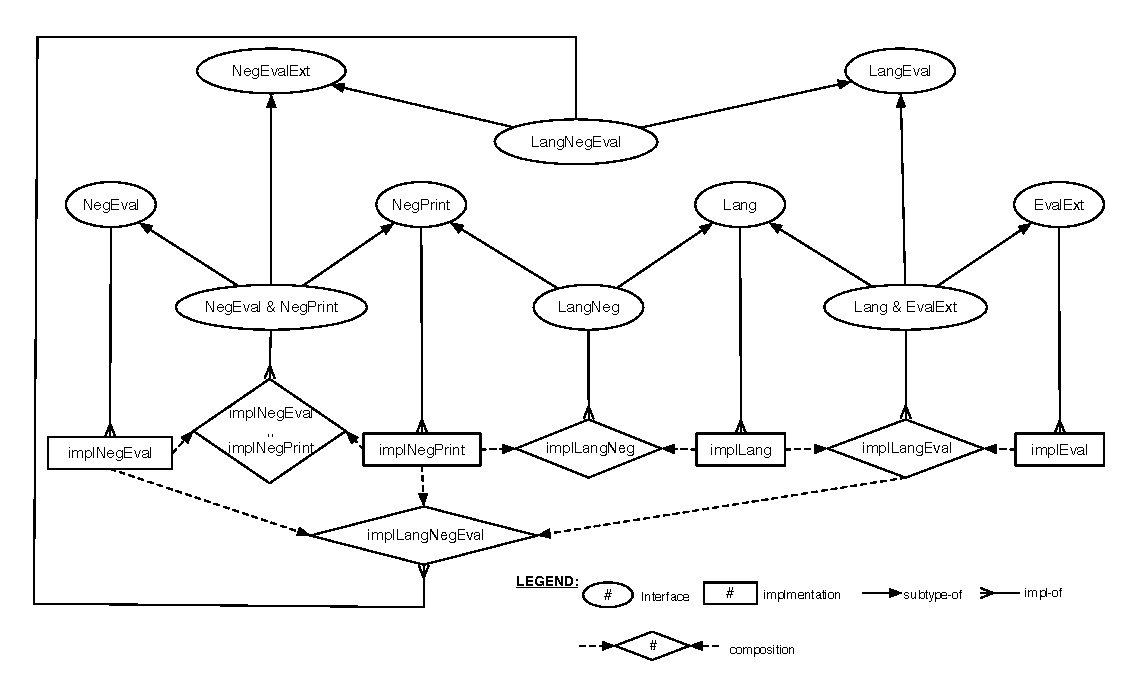
\includegraphics[scale=0.75]{figures/diagram.eps}
\caption{Summary of the relationships between language components}
\label{fig:diagram}
\end{figure}


\paragraph{Stand-alone extensions.}
Unlike in \textsf{gbeta} and other class-based inheritance systems, in \namee
the extension \lstinline{implEval} is not tied to \lstinline{LangEval}. In that
sense, it resembles trait and mixin systems that can apply the same extension
to different classes. However, unlike those systems, \lstinline{implEval} can also
exist as a value on its own, i.e., it is not an extension per se.

%-------------------------------------------------------------------------------
% \subsection{Disjoint Intersection Types and Ambiguity}

% The above example shows that intersection types and the merge operator
% are closely related to multiple
% inheritance. Indeed, they share a major concern with multiple inheritance,
% namely ambiguity. When a subclass inherits an implementation of the same
% method from two different parent classes, it is unclear which of the two
% methods is to be adopted by the subclass. In the case where the two parent classes
% have a common superclass, this is known as the \emph{diamond problem}.
% The ambiguity problem also appears in \namee,
% e.g., if we merge two numbers to obtain $\mer{1}{2}$ of type
% $\inter{\mathsf{Int}}{\mathsf{Int}}$. Is the result of $\mer{1}{2} + 3$
% either $4$ or $5$?

% Disjoint intersection types offer to statically detect potential ambiguity and
% to ask the programmer to explicitly resolve the ambiguity by rejecting the
% program in its ambiguous form. In the previous work on \oname, ambiguity is
% avoided by dictating that all intersection types have to be disjoint, i.e.,
% $\inter{\mathsf{Int}}{\mathsf{Int}}$ is ill-formed because the first component
% has the same type as the second.


% Disjoint intersection types ensure unambiguity and conflicts are
% statically detected and manually resolved by programmers. This
% is similar to the trait model.


% Local Variables:
% TeX-master: "../../Thesis"
% org-ref-default-bibliography: ../../Thesis.bib
% End:


\newcommand{\rulehl}[2][gray!40]{%
  \colorbox{#1}{$\displaystyle#2$}}

\section{Syntax and Semantics}
\label{sec:typesystem}

In this section we formally present the syntax and semantics of \namee. Compared
to prior work~\cite{alpuimdisjoint, oliveira2016disjoint}, \namee has a more
powerful subtyping relation. The new subtyping relation is inspired by BCD-style
subtyping, but with two noteworthy differences: subtyping is coercive (in
contrast to traditional formulations of BCD); and it is extended with records.
We also have a new target language with explicit coercions inspired by the coercion calculus of
Henglein~\cite{Henglein_1994}. A full technical comparison between \namee and \oname can be found in \cref{sec:comparision}.


\subsection{Syntax}

\Cref{fig:source} shows the syntax of \namee.
% with the differences from \oname \hll{highlighted}.
% \namee is a simple calculus with intersection types, the merge operator
% and singleton records.
For brevity of the meta-theoretic study, we do not
consider primitive operations on integers, or other primitive types.
They can be easily added to the language, and our prototype implementation is
indeed equipped with common primitive types and their operations.
Metavariables $[[A]], [[B]], [[C]]$ range over types. Types include the type of integers
$[[nat]]$, a top type $[[Top]]$, function types $[[A -> B]]$, intersection types
$[[A & B]]$, and singleton record types $[[ {l : A} ]]$. Metavariable $[[ee]]$
ranges over expressions. Expressions include variables $[[x]]$, integers $[[i]]$,
a canonical top value $[[Top]]$, lambda abstractions $[[\x . ee]]$,
applications $[[ee1 ee2]]$, merges $[[ee1 ,, ee2]]$, annotated terms $[[ee : A]]$,
singleton records $[[ {l = ee}]]$, and record selections $[[ee.l ]]$.

\begin{figure}[t]
  \centering
\begin{tabular}{llll}\toprule
  Types & $[[A]], [[B]], [[C]]$ & $\Coloneqq$ & $[[nat]] \mid [[Top]] \mid [[A -> B]]  \mid [[A & B]] \mid [[ { l : A } ]]$ \\
  Expressions & $[[ee]]$ & $\Coloneqq$ & $[[x]] \mid [[i]] \mid [[Top]] \mid [[\x . ee]] \mid [[ee1 ee2]] \mid [[ee1 ,, ee2]] \mid [[ee : A]]  $ \\
  & & $\mid$ & $ [[ { l = ee } ]] \mid [[ee.l]] $ \\
  Typing contexts & $[[GG]]$ & $\Coloneqq$ & $[[empty]] \mid [[GG , x : A]]$ \\ \bottomrule
\end{tabular}
  \caption{Syntax of \namee}
  \label{fig:source}
\end{figure}

\subsection{Declarative Subtyping}

\Cref{fig:subtype_decl} presents the subtyping relation. We ignore the
\hll{highlighted} parts, and explain them later in \cref{sec:elaboration}.

\begin{figure}[t]
  \centering
  \drules[S]{$[[A <: B ~~> c]]$}{Declarative subtyping}{refl, trans, top, rcd, arr, andl, andr, and, distArr, topArr, distRcd, topRcd}
  \caption{Declarative specification of subtyping}
  \label{fig:subtype_decl}
\end{figure}

\paragraph{BCD-Style Subtyping.}
The subtyping rules are essentially those of the BCD type
system~\cite{Barendregt_1983}, extended with subtyping for singleton records.
\Rref{S-top,S-rcd} for top types and record types are straightforward.
\Rref{S-arr} for function subtyping is standard. \Rref{S-andl,S-andr,S-and} for
intersection types axiomatize that $[[A & B]]$ is the greatest lower bound of
$[[A]]$ and $[[B]]$. \Rref{S-distArr} is perhaps the most interesting rule.
This, so-called ``distributivity'' rule, describes the interaction between
the subtyping relations for function types and those for intersection types.
Note that the other direction $[[A1 -> A2 & A3 <: (A1 -> A2) & (A1 -> A3)]]$
and the contravariant distribution $[[ (A1 -> A2) & (A3 -> A2) <: A1 & A3 -> A2 ]]$ are both
derivable from the existing subtyping rules, as shown below:
  \begin{footnotesize}
\begin{mathpar}
  \inferrule*[right=\rref*{S-and}]
  {  \inferrule*[right=\rref*{S-arr}]{ [[ A1 <: A1  ]] \\ [[ A2 & A3 <: A2  ]]  }{[[   A1 -> A2 & A3 <: A1 -> A2  ]]} \\
    \inferrule*[right=\rref*{S-arr}]{ [[ A1 <: A1  ]] \\ [[ A2 & A3 <: A3  ]] }{[[ A1 -> A2 & A3 -> A1 -> A3      ]]}  }
  {  [[ A1 -> A2 & A3 <: (A1 -> A2) & (A1 -> A3)  ]]  }
\end{mathpar}
\begin{mathpar}
  \inferrule*[right=\rref*{S-trans}]
  {  \inferrule*[right=\rref*{S-andl}]{ }{[[ (A1 -> A2) & (A3 -> A2) <: A1 -> A2   ]]} \\
    \inferrule*[right=\rref*{S-arr}]{ [[ A1 & A3 <: A1  ]] \\ [[ A2 <: A2  ]] }{[[ A1 -> A2 <: A1 & A3 -> A2  ]]}  }
  {  [[  (A1 -> A2) & (A3 -> A2) <: A1 & A3 -> A2  ]]   }
\end{mathpar}
  \end{footnotesize}
\Rref{S-distRcd}, which is not found in the original BCD system,
prescribes the distribution of records over intersection types. The two
distributivity rules are the key to enable nested composition. The rule
\rref*{S-topArr} is standard in BCD subtyping, and the new
\rref{S-topRcd} plays a similar role for record types.

\paragraph{Non-Algorithmic.}
The subtyping relation in \cref{fig:subtype_decl} is clearly no more than a
specification due to the two subtyping axioms: \rref{S-refl,S-trans}. A sound
and complete algorithmic version is discussed in \cref{sec:alg}. Nevertheless,
for the sake of establishing coherence, the declarative subtyping relation is
sufficient.


\paragraph{Property of Subtyping.}
The subtyping relation is vacuously \textit{reflexive} and \textit{transitive}.



\subsection{Typing of \namee}


\begin{figure}[t]
  \centering
\drules[T]{$[[GG  |- ee => A ~~> e]]$}{Inference}{top, lit, var, app, anno, proj, merge, rcd}
\drules[T]{$[[GG  |- ee <= A ~~> e]]$}{Checking}{abs, sub}
  \caption{Bidirectional type system of \namee}
  \label{fig:type_system}
\end{figure}

% no gray anymore after this point
\renewcommand{\rulehl}[1]{#1}



The bidirectional type system for \namee is shown in \cref{fig:type_system}.
Again we ignore the \hll{highlighted} parts for now.

% The main difference to \oname is the absence of a well-formedness
% judgement. Unlike \oname, which requires a well-formedness judgement to ensure
% that all intersection types are disjoint, \namee only requires a disjointness
% check at the merge operator. Non-disjoint types such as $[[nat & nat]]$ are
% allowed in other parts of the program.

\begin{comment}
Unlike the development of \oname, which first presents a type assignment
specification, \Cref{fig:type_system} directly present the bidirectional type
system of \namee.
Unfortunately, we found that their declarative type
system is incoherent in nature (even with all the syntactic restrictions).
\jeremy{perhaps add a counter example somewhere?} Again, the reader is advised
to continue ignoring the gray-shaded parts until \cref{sec:elaboration}.
\tom{The above story is a bit confusing to me. Is it the case that the
     \oname paper already was aware of the coherence problem with its
     declarative type system and for that reason (and inference) presented
     a bidirection type system as well? If so, that's not clear.} \jeremy{I
     remember at one point Bruno and I believed the declarative system is
     coherent, it's just hard to prove. Then I found a counterexample. That was
     after \tname paper.  }
\end{comment}


\begin{figure}[t]
  \centering
  \drules[D]{$[[A ** B]]$}{Disjointness}{topL, topR, arr, andL, andR, rcdEq, rcdNeq,ax}
  \drules[Dax]{$[[A **a B]]$}{Disjointness axioms}{sym, intArr, intRcd,arrRcd}
  \caption{Disjointness}
  \label{fig:disjoint}
\end{figure}


\paragraph{Typing Rules and Disjointness.}

As with traditional bidirectional type systems, we employ two modes: the
inference mode ($[[=>]]$) and the checking mode ($[[<=]]$). The inference
judgement $[[GG |- ee => A]]$ says that we can synthesize a type $[[A]]$ for
expression $[[ee]]$ in the context $[[GG]]$. The checking judgement $[[GG |- ee
<= A]]$ checks $[[ee]]$ against $[[A]]$ in the context $[[GG]]$. The
disjointness judgement $[[A ** B]]$ used in \rref{T-merge} is shown in
\cref{fig:disjoint}, which states that the types $[[A]]$ and $[[B]]$ are
\textit{disjoint}. The intuition of two types being disjoint is
that their least upper bound is (isomorphic to) $[[Top]]$. The disjointness judgement is
important in order to rule out ambiguous expressions such as $\mer{1}{2}$. Most
of the typing and disjointness rules are standard and are explained in detail in
previous work~\cite{oliveira2016disjoint, alpuimdisjoint}.
%We refer
%the reader to their papers for further explanation.


\subsection{Elaboration Semantics}
\label{sec:elaboration}

\begin{figure}[t]
  \centering
\begin{tabular}{llll} \toprule
  Types & $[[T]]$ & $\Coloneqq$ & $[[nat]] \mid [[Unit]] \mid [[T1 * T2]] \mid [[T1 -> T2]] $ \\
  Terms & $[[e]]$ & $\Coloneqq$ & $[[x]] \mid [[i]] \mid [[unit]] \mid [[\x . e]] \mid [[e1 e2]] \mid [[<e1, e2>]] \mid [[c e]]$ \\
  Coercions & $[[c]]$ & $\Coloneqq$ & $ [[id]] \mid [[c1 o c2]] \mid [[top]] \mid [[c1 -> c2]] \mid [[<c1, c2>]] \mid [[pp1]] \mid [[pp2]] $ \\
  &  &  $\mid$ & $   [[distArr]] \mid [[topArr]]  $ \\
  Values & $[[v]]$ & $\Coloneqq$ & $[[unit]] \mid [[i]] \mid [[\x.e]] \mid  [[<v1, v2>]] \mid [[(c1 -> c2) v]] \mid [[distArr v]] \mid [[topArr v]] $ \\
  Typing contexts & $[[gg]]$ & $\Coloneqq$ & $[[empty]] \mid [[gg , x : T]]$ \\
  Evaluation Contexts & $[[EE]]$ & $\Coloneqq$ &  $  [[__]] \mid [[EE e]] \mid [[v EE]] \mid [[ < EE , e >  ]] \mid [[ < v , EE > ]] \mid [[ c EE  ]]$ \\ \bottomrule
\end{tabular}
  \caption{\tname syntax}
  \label{fig:target}
\end{figure}

The operational semantics of \namee is given by elaborating source expressions
$[[ee]]$ into target terms $[[e]]$. Our target language \tname is the standard
simply-typed call-by-value $\lambda$-calculus extended with products and coercions.
The syntax of \tname is shown in \cref{fig:target}. The
meta-function $| \cdot |$ shown in \cref{def:type:translate} transforms \namee
types to \tname types, and extends naturally to typing contexts.

\begin{definition}[Type translation from \namee to \tname] \label{def:type:translate}
  \begin{align*}
    | [[nat]] | &= [[nat]] \\
    | [[Top]] | &= \langle \rangle \\
    | [[A -> B]]  | &= [[ | A | -> | B |  ]] \\
    | [[ A & B  ]] | &= [[ | A | * | B |  ]] \\
    | \recordType{l}{A} | &= | A |
  \end{align*}
\end{definition}



\paragraph{Explicit Coercions and Coercive Subtyping.}

The separate syntactic category for explicit coercions is a distinct
difference from the prior works (in which they are regular terms). Our coercions
are based on those of Henglein~\cite{Henglein_1994}, and we add more forms due to our
extra subtyping rules.
Metavariable $[[c]]$ ranges over coercions.\footnote{Coercions $[[pp1]]$ and $[[pp2]]$ subsume the first and second projection of pairs, respectively.}
Coercions express the conversion
of a term from one type to another. Because of the addition of coercions, the
grammar contains explicit coercion applications $[[c e]]$ as a term, and various
unsaturated coercion applications as values. The use of explicit coercions is useful for the new semantic
proof of coherence based on logical relations.
The subtyping judgement in \cref{fig:subtype_decl} has the form $[[A <: B ~~> c]]$, which says that the
subtyping derivation of $[[A <: B]]$ produces a coercion $[[c]]$ that converts
terms of type $[[ |A| ]]$ to type $[[ |B| ]]$. Each subtyping rule has its own
specific form of coercion.

%The meaning of the different forms of coercions becomes clear in \tom{Section
%  TODO} \jeremy{it's a paragraph, how to refer it?} which explains coercive
%subtyping.\bruno{Why not discuss the form of coercions directly here?}


\paragraph{Target Typing.}
The typing of \tname has the form $[[gg |- e : T]]$, which is entirely standard. Only the typing of coercion
applications, shown below, deserves attention:
\begin{mathpar}
\drule{t-capp}
\end{mathpar}
Here the judgement $[[c |- T1 tri T2]]$ expresses the typing of coercions, which
are essentially functions from $[[T1]]$ to $[[T2]]$. Their typing
rules correspond exactly to the subtyping rules of \namee, as
shown in \cref{fig:co}.

\begin{figure}[t]
  \centering
  \drules[ct]{$[[c |- T1 tri T2]]$}{Coercion typing}{refl, trans, top, topArr, arr, pair, projl, projr, distArr}
  \caption{Coercion typing}
  \label{fig:co}
\end{figure}

\paragraph{Dynamic Semantics.}

\begin{figure}[t]
  \centering
\drules[r]{$[[e --> e']]$}{Single-step reduction}{id, trans, top, topArr, pair, arr, distArr, projl, projr, app, ctxt}
  \caption{Dynamic semantics of \tname}
  \label{fig:coercion_red}
\end{figure}

The dynamic semantics of \tname is shown in \cref{fig:coercion_red}. We write
$[[e --> e']]$ for reduction of expressions. The first three lines are reduction
rules for coercions. They do not contribute to computation but merely rearrange
coercions. Our coercion reduction rules are quite standard but not efficient in
terms of space. Nevertheless, there is existing work on space-efficient
coercions~\cite{Siek_2015, herman2010space}, which should be applicable to our
work as well. \Rref{r-app} is the usual $\beta$-rule that performs actual
computation, and \rref{r-ctxt} handles reduction under an evaluation context. As
standard, $[[-->>]]$ is the reflexive, transitive closure of $[[-->]]$.
Now we can show that \tname is type safe:
\begin{theorem}[Preservation]
  If $[[empty |- e : T]]$ and $[[e --> e']]$, then $[[empty |- e' : T]]$.
\end{theorem}
\begin{theorem}[Progress]
  If $[[empty |- e : T]]$, then either $[[e]]$ is a value, or there exists $[[e']]$ such
  that $[[e --> e']]$.
\end{theorem}




\paragraph{Elaboration.}
\begin{comment}
The subtyping judgement in \cref{fig:subtype_decl} has the form $[[A <: B ~~> c]]$, which says that the subtyping
derivation of $[[A <: B]]$ produces a coercion $[[c]]$ that is used to convert a
term of type $[[ |A| ]]$ to type $[[ |B| ]]$. Each
subtyping rule has its own specific form of coercion.
\end{comment}
We are now in a position to explain the elaboration judgements $[[GG |- ee
=> A ~~> e]]$ and $[[GG |- ee <= A ~~> e]]$ in \cref{fig:type_system}. The only
interesting rule is \rref{T-sub}, which applies the coercion $[[c]]$ produced by
subtyping to the target term $[[e]]$ to form a coercion application
$[[c e]]$. All the other rules do straightforward translations between
source and target expressions.


To conclude, we show two lemmas that relate \namee expressions
to \tname terms.
% (Note that in this and subsequent sections, we only provide
% a proof sketch for each lemma and theorem. We refer the interested reader
% to our Coq development for the full proofs.)

\begin{lemma}[Coercions preserve types]
  If $[[A <: B ~~> c]]$, then $[[c |-  |A| tri |B|]]$.
  \label{lemma:sub-correct}
\end{lemma}
\begin{proof}
  By structural induction on the derivation of subtyping.
\end{proof}


\begin{lemma}[Elaboration soundness] We have that:
  \begin{itemize}
  \item If $[[GG |- ee => A ~~> e]]$, then $|\Gamma| \vdash e : |A| $.
  \item If $[[GG |- ee <= A ~~> e]]$, then $|\Gamma| \vdash e : |A| $.
  \end{itemize}
\end{lemma}
\begin{proof}
  By structural induction on the derivation of typing.
\end{proof}

\subsection{Comparison with \oname}
\label{sec:comparision}

Below we identify major differences between \namee and \oname, which, when
taken together, yield a simpler and more elegant system. The differences may seem
superficial, but they have far-reaching impacts on the semantics, especially on
coherence, our major topic in \cref{chap:coherence:simple}.

\paragraph{No Ordinary Types.}

Apart from the extra subtyping rules, there is an important difference from the
\oname subtyping relation. The subtyping relation of \oname employs an
auxiliary unary relation called $\mathsf{ordinary}$, which plays a fundamental
role for ensuring coherence and obtaining an
algorithm~\cite{Davies_2000}. The \namee calculus discards the notion of
ordinary types completely; this yields a clean and elegant formulation of the
subtyping relation. Another minor difference is that due to the addition of the
transitivity axiom (\rref{S-trans}), \rref{S-andl,S-andr} are simplified: an
intersection type $[[A & B]]$ is a subtype of both $[[A]]$ and $[[B]]$, instead
of the more general form $[[ A & B <: C]]$.

% \paragraph{Example}
% The following example shows the derivation tree of the subtyping example
% presented in \cref{sec:overview}. \jeremy{A derivation of the nested composition
%   example? }


\paragraph{No Top-Like Types.}

There is a notable difference from the coercive subtyping of \oname. Because of
their syntactic proof method, they have special treatment for coercions of
\textit{top-like types} in order to retain coherence. For \namee, as
with ordinary types, we do not need this kind of ad-hoc treatment, thanks to the
adoption of a more powerful proof method (cf. \cref{chap:coherence:simple}).




\paragraph{No Well-Formedness Judgement.}

A key difference from the type system of \oname is the complete omission of the
well-formedness judgement. In \oname, the well-formedness judgement $[[GG |- A]]$
appears in both \rref{T-abs,T-sub}. The sole purpose of this judgement is
to enforce the invariant that all intersection types are disjoint. However, as
\cref{chap:coherence:simple} will explain, the syntactic restriction is unnecessary for
coherence, and merely complicates the type system. The \namee calculus discards
this well-formedness judgement altogether in favour of a simpler design that is
still coherent. An important implication is that even without adding BCD subtyping,
\namee is already more expressive than \oname: an expression such as $1 : [[nat & nat]]$ is accepted in
\namee but rejected in \oname. This simplification is based on an important
observation: incoherence can only originate in merges. Therefore disjointness
checking is only necessary in \rref{T-merge}.


% Local Variables:
% TeX-master: "../../Thesis"
% org-ref-default-bibliography: ../../Thesis.bib
% End:


\section{Algorithmic Subtyping}
\label{sec:alg}

This section presents an algorithm that implements the subtyping relation in
\cref{fig:subtype_decl}. While BCD subtyping is well-known, the
presence of a transitivity axiom in the rules means that the system is
not algorithmic. This raises an obvious question: how to obtain an
algorithm for this subtyping relation? Laurent~\cite{Laurent12note} has shown that simply dropping
the transitivity rule from the BCD system is not possible without losing expressivity. Hence, this avenue for
obtaining an algorithm is not available. 
%Moreover, even if transitivity elimination
%would be possible, the remaining rules are still highly overlapping, and pose
%difficulties for an implementation.  
Instead, we adapt Pierce's decision
procedure~\cite{pierce1989decision} for a subtyping system (closely
related to BCD) to obtain a sound and complete algorithm for our
BCD extension. Our algorithm extends Pierce's decision
procedure with subtyping of singleton records and
coercion generation. We prove in Coq that the algorithm is sound and complete with
respect to the declarative version. At the same time we
find some errors and missing lemmas in Pierce's original manual proofs.

%The algorithm is implemented in our
%prototype implementation. \jeremy{should i say more about implementation?}

%See \cref{sec:alg} for the details. 
%\bruno{The meaning of the paragraph is somewhat obscure to me. After
%  discussing with Tom, it seems that what may be meant here is that we
%cannot do cut elimination, which is a common process that you can try
%for certain systems with subtyping. However Pierce managed to find
%another way to get a sound/complete algorithmic system. Maybe 
%the text can be improved.}


\subsection{The Subtyping Algorithm}

\begin{figure}[t]
  \centering
  \begin{small}
  \drules[A]{$[[fs |- A <: B ~~> c]]$}{Algorithmic subtyping}{and, arr, rcd, top, arrNat, rcdNat, andNOne, andNTwo, nat}
  \end{small}
  \caption{Algorithmic subtyping of \name}
  \label{fig:algorithm}
\end{figure}


\Cref{fig:algorithm} shows the algorithmic subtyping judgement $[[fs |- A <: B ~~> c]]$.
This judgement is the algorithmic counterpart of the declarative
judgement $[[A <: fs -> B ~~> c]]$, where the symbol $[[fs]]$ stands for a
queue of types and labels. Definition~\ref{def:fs} converts a queue to a type:
\begin{definition} $[[fs -> A]]$ is inductively defined as follows: \label{def:fs}
  \begin{mathpar}
    [[ [] -> A]] = [[A]] \and
    [[ (fs , B) -> A]] = [[fs -> (B -> A)]] \and
    [[ (fs , {l}) -> A]] = [[fs -> {l : A}]]
  \end{mathpar}
\end{definition}
For instance, if $[[fs]] = [[A]] , [[B]] , \{[[l]]\} $, then $[[fs -> C]]$ abbreviates $ [[A -> B -> {l : C}]]$.

The basic idea of $[[fs |- A <: B ~~> c]]$ is to first perform a structural
analysis of $[[B]]$, which descends into both sides of $[[&]]$'s (\rref{A-and}),
into the right side of $[[->]]$'s (\rref{A-arr}), and into the fields of records
(\rref{A-rcd}) until it reaches one of the two base cases, $[[nat]]$ or
$[[Top]]$. If the base case is $[[Top]]$, then the subtyping holds trivially
(\rref{A-top}). If the base case is $[[nat]]$, the algorithm performs a
structural analysis of $[[A]]$, in which $[[fs]]$ plays an important role. The
left sides of $[[->]]$'s are pushed onto $[[fs]]$ as they are encountered in
$[[B]]$ and popped off again later, left to right, as $[[->]]$'s are encountered
in $[[A]]$ (\rref{A-arrNat}). Similarly, the labels are pushed onto $[[fs]]$ as
they are encountered in $[[B]]$ and popped off again later, left to right, as
records are encountered in $[[A]]$ (\rref{A-rcdNat}). The remaining rules are
similar to their declarative counterparts. Let us illustrate the algorithm
with an example
derivation (for space reasons we use $[[N]]$ and $[[S]]$ to denote $[[nat]]$ and $[[string]]$ respectively),
which is essentially the one used by the \lstinline{add} field in \cref{sec:overview}. The
readers can try to give a corresponding derivation using the declarative
subtyping and see how \rref{S-trans} plays an essential role there.
\begin{small}
\begin{mathpar}
  \inferrule*[right=\rref*{A-rcd}]
  { \inferrule*[right=\rref*{A-arr}(\textit{twice})]
    { \inferrule*[right=\rref*{A-and}]
      { D \\ D' }
      { \{ [[l]]  \}, [[N & S]] ,[[N & S]] \vdash [[{l : N -> N -> N} & {l : S -> S -> S} ]] \prec : [[N & S]] }  }
    { \{ [[l]]  \} \vdash [[{l : N -> N -> N} & {l : S -> S -> S} ]] \prec : [[ N & S -> N & S -> N & S ]]}      }
  {  [[{l : N -> N -> N} & {l : S -> S -> S}]] \prec : [[{l : N & S -> N & S -> N & S}]]   }
\end{mathpar}
\end{small}
where the sub-derivation $D$ is shown below ($D'$ is similar):
\begin{small}
\begin{mathpar}
\inferrule*[right=\rref*{A-andN1}]
        { \inferrule*[right=\rref*{A-rcdNat}]
          { \inferrule*[right=\rref*{A-arrNat}]
            { \inferrule*{ \dots } { [[N & S]] \prec : [[N]] }
              \\
              \inferrule* {\dots} { [[N & S]] \vdash [[N -> N]] \prec : [[N]] }     }
            {[[N & S]] ,[[N & S]] \vdash [[N -> N -> N]] \prec : [[N]]} }
          { \{ [[l]]  \}, [[N & S]] ,[[N & S]] \vdash [[{l : N -> N -> N}]] \prec : [[N]] } }
        { \{ [[l]]  \}, [[N & S]] ,[[N & S]] \vdash [[{l : N -> N -> N} & {l : S -> S -> S} ]] \prec : [[N]] }
\end{mathpar}
\end{small}
Now consider the coercions. Algorithmic subtyping uses the same set of
coercions as declarative subtyping. However, because algorithmic
subtyping has a different structure, the rules generate slightly more
complicated coercions. Two meta-functions $\llbracket \cdot \rrbracket_{\top}$
and $\llbracket \cdot \rrbracket_{\&}$ used in \rref{A-top,A-and} respectively,
are meant to generate correct forms of coercions. They are defined recursively
on $[[fs]]$ and are shown in \cref{fig:coercion}.

\begin{figure}[t]
    \centering
    \begin{small}
    \begin{subfigure}[b]{0.5\textwidth}
      \begin{align*}
        [[ < [] >1 ]] &=  [[top]] \\
        [[ < { l } , fs >1 ]] &= [[ {l : < fs >1} o < l >  ]] \\
        [[ < A , fs >1 ]] &= [[(top -> < fs >1) o (topArr o top)]]
      \end{align*}
    \end{subfigure} ~
    \begin{subfigure}[b]{0.45\textwidth}
      \begin{align*}
        [[ < [] >2 ]] &=  [[id]] \\
        [[ < { l } , fs >2 ]] &= [[ {l : < fs >2} o distRcd l  ]] \\
        [[ < A , fs >2 ]] &= [[(id -> < fs >2) o distArr]]
      \end{align*}
    \end{subfigure}
    \end{small}
    \caption{Meta-functions of coercions}\label{fig:coercion}
\end{figure}

\subsection{Correctness of the Algorithm}

To establish the correctness of the algorithm, we must show that the algorithm
is both sound and complete with respect to the declarative specification. While
soundness follows quite easily, completeness is much harder. The proof of
completeness essentially follows that of Pierce~\cite{pierce1989decision}
%%\footnote{
%%While transferring \cite{pierce1989decision}'s manual proofs to Coq,
%%we discovered several errors, which will be reported along the way.}
in that we
need to show the algorithmic subtyping is reflexive and
transitive. 


\paragraph{Soundness of the Algorithm.}

The following two lemmas connect the declarative subtyping with the meta-functions.

\begin{lemma} \label{lemma:top}
  $[[ Top <: fs -> Top ~~> < fs >1]]$
\end{lemma}
\begin{proof}
  By induction on the length of $[[fs]]$.
\end{proof}

\begin{lemma} \label{lemma:and}
  $[[(fs -> A) & (fs -> B) <: fs -> (A & B) ~~> < fs >2]]$
\end{lemma}
\begin{proof}
  By induction on the length of $[[fs]]$.
\end{proof}

The proof of soundness is straightforward.
\begin{theorem}[Soundness] \label{thm:soundness}
  If $[[ fs |- A <: B ~~> c]]$ then $[[A]] <: [[fs]] \rightarrow [[B]] [[~~>]] [[c]]$.
\end{theorem}
\begin{proof}
  By induction on the derivation of the algorithmic subtyping and applying \cref{lemma:top,lemma:and} where appropriate.
\end{proof}


\paragraph{Completeness of the Algorithm.}


\newcommand{\UU}[1]{\mathcal{U}(#1)}

Completeness, however, is much harder. The reason is that, due to the use of
$[[fs]]$, reflexivity and transitivity are not entirely obvious. We need to
strengthen the induction hypothesis by introducing the notion of a set,
$\UU{[[A]]}$, of ``reflexive supertypes'' of $[[A]]$, as defined below:
\begin{mathpar}
  \UU{[[Top]]} \defeq \{ [[Top]]  \} \and
  \UU{[[nat]]} \defeq \{ [[nat]]  \} \and
  \UU{[[{l : A}]]} \defeq \{ [[{l : B}]] \mid [[B]] \in \UU{[[A]]}  \} \and
  \UU{[[A & B]]} \defeq \UU{[[A]]} \cup \UU{[[B]]} \cup \{ [[A & B]] \} \and
  \UU{[[A -> B]]} \defeq \{ [[A -> C]] \mid [[C]] \in \UU{[[B]]} \}
\end{mathpar}
We show two lemmas about $\UU{[[A]]}$ that are crucial in the subsequent proofs.
\begin{lemma} \label{lemma:set_refl}
  $[[A]] \in \UU{[[A]]}$
\end{lemma}
\begin{proof}
  By induction on the structure of $[[A]]$.
\end{proof}

\begin{lemma} \label{lemma:set_trans}
  If $[[A]] \in \UU{[[B]]}$ and $[[B]] \in \UU{[[C]]}$, then $[[A]] \in \UU{[[C]]}$.
\end{lemma}
\begin{proof}
  By induction on the structure of $[[B]]$.
\end{proof}

\begin{remark}
  Lemma~\ref{lemma:set_trans} is not found in Pierce's proofs~\cite{pierce1989decision}, which is
  crucial in Lemma~\ref{lemma:refl0}, from which reflexivity (Lemma~\ref{lemma:refl})
  follows immediately.
\end{remark}

% Next we show the following lemma from which reflexivity (Lemma~\ref{lemma:refl})

\begin{lemma} \label{lemma:refl0}
  If $[[fs -> B]] \in \UU{[[A]]}$ then there exists $[[c]]$ such that $[[fs |- A <: B ~~> c]]$.
\end{lemma}
\begin{proof}
  By induction on $\mathsf{size}([[A]]) + \mathsf{size}([[B]]) + \mathsf{size}([[fs]])$.
\end{proof}
% \begin{remark}
%   \cite{pierce1989decision}'s proof is wrong in one case~\cite[pp.~10, Case~ii]{pierce1989decision} because we need \cref{lemma:set_trans} to be able
%   to apply the inductive hypothesis.
% \end{remark}

Now it immediately follows that the algorithmic subtyping is reflexive.

\begin{lemma}[Reflexivity] \label{lemma:refl}
  For every $[[A]]$ there exists $[[c]]$ such that $[[ [] |- A <: A ~~> c]]$.
\end{lemma}
\begin{proof}
  Immediate from Lemma~\ref{lemma:set_refl} and Lemma~\ref{lemma:refl0}.
\end{proof}

We omit the details of the proof of transitivity.
%The proof of transitivity is, to quote \cite{pierce1989decision}, typically
%``the hardest single piece'' of metatheory. We omit the details here for lack of space and
%refer the interested reader to our Coq development.

\begin{lemma}[Transitivity] \label{lemma:trans}
  If $[[ [] |- A1 <: A2 ~~> c1]]$ and $[[ [] |- A2 <: A3 ~~> c2]]$, then there
  exists $[[c]]$ such that $[[ [] |- A1 <: A3 ~~> c]]$.
\end{lemma}

With reflexivity and transitivity in position, we show the main theorem.

\begin{theorem}[Completeness] \label{thm:complete}
  If $[[A <: B ~~> c]]$ then there exists $[[c']]$ such that $[[ [] |- A <: B ~~> c']]$.
\end{theorem}
\begin{proof}
  By induction on the derivation of the declarative subtyping and applying \cref{lemma:refl,lemma:trans} where appropriate.
\end{proof}
\begin{remark}
  Pierce's proof is wrong~\cite[pp.~20, Case~F]{pierce1989decision} in the case
  \begin{mathpar}
  \drule{S-arr}
  \end{mathpar}
  where he concludes from the inductive
  hypotheses $[[ [] |- B1 <: A1]]$ and $[[ [] |- A2 <: B2]]$ that $[[ [] |- A1 -> A2 <: B1 -> B2]]$ (rules 6a and 3).
  However his rule 6a (our \rref{A-arrNat}) only works for \textit{primitive types}, and is thus not applicable in this case. Instead we
  need a few technical lemmas to support the argument.
\end{remark}

\begin{remark}
  It is worth pointing out that the two coercions $[[c]]$ and $[[c']]$ in
  Theorem~\ref{thm:complete} are contextually equivalent, which follows from
  Theorem~\ref{thm:soundness} and Corollary~\ref{lemma:coercion_same}.
\end{remark}

% Local Variables:
% org-ref-default-bibliography: ../paper.bib
% End:

% 
\section{Conclusions and Future Work}
\label{sec:conclusion}

We have proposed \name, a type-safe and coherent calculus with disjoint
intersection types, and support for nested composition/subtyping. \name
improves upon earlier work with a more
flexible notion of disjoint intersection types, which leads to
a clean and elegant formulation of the type system. Due to the added
flexibility we have had to employ a more powerful proof method based on logical
relations to rigorously prove coherence.
We also show how \name supports essential features of family
polymorphism, such as nested composition. We believe \name provides insights into family polymorphism, and
has potential for practical applications for extensible software designs.

A natural direction for future work is to enrich \name with parametric
polymorphism. There is abundant literature on logical relations for parametric
polymorphism~\cite{reynolds1983types} and we foresee no fundamental difficulties
in extending our proof method.\footnote{ Our prototype implementation already
  supports polymorphism, but we are still in the process of extending our Coq
  development with polymorphism.} The main challenge in the definition of the
logical relation is the clause for type variables with arbitrary types. Careful
measures are to be taken to avoid the potential circularity due to
impredicativity. With the combination of parametric polymorphism and nested
composition, an interesting application that we intend to investigate is native
support for a highly modular form of \textit{Object Algebras}~\cite{oliveira2012extensibility, xuan_traits} and \textsc{Visitor}s
(or the finally tagless approach~\cite{CARETTE_2009}).

Another direction for future work is to add mutable references, which would
touch two places in our metatheory: type safety and coherence. For type safety,
we expect that lessons learned from previous work on family polymorphism and
mutability on OO to apply to our work. For example, it is well-known that
subtyping in the presence of mutable state often needs restrictions. Given such
suitable restrictions we expect that type-safety in the presence of mutability
still works. For coherence, it would be a major technical challenge to adjust
our coherence proof and its Coq mechanisation. Logical relations that account
for mutable state (e.g., see Ahmed's thesis~\cite{ahmed2004semantics}) introduce significant complexity.





% For example, we can
% define the object algebra interfaces for the Expression Problem example in
% \cref{sec:overview} as follows:
% \lstinputlisting[linerange=77-78]{../../impl/examples/overview.sl}% APPLY:linerange=LANG_EXT_INTER
% By instantiating \lstinline{E} with \lstinline{IPrint}, i.e.,
% \lstinline{ExpAlg[IPrint]}, we get the interface of the \lstinline{Lang} family.
% In that sense, object algebra interfaces can be viewed as family interfaces.
% Moreover, combining algebras implementing \lstinline{ExpAlg[IPrint]} and
% \lstinline{ExpAlg[IEval]} to form \lstinline{ExpAlg[IPrint & IEval]} is trivial
% with nested composition. Polymorphism also improves code reuse across expressions in the
% base and extended languages. For example, the following creates two expressions,
% one in the base language, the other in the extended language:
% \lstinputlisting[linerange=83-84]{../../impl/examples/overview.sl}% APPLY:linerange=LANG_EXT
% Notice how we can  reuse \lstinline{e1} of the base language in the definition
% of \lstinline{e2}.



% \jeremy{creating expressions using base and extended expressions, and show more reuse}

% \jeremy{future work} \jeremy{mention in passing this rule is unsound with
%   effects, see ``Intersection types and computational effects''}

% Local Variables:
% mode: latex
% TeX-master: "../paper"
% org-ref-default-bibliography: ../paper.bib
% End:




%%% Local Variables:
%%% mode: latex
%%% TeX-master: "../Thesis"
%%% End:

  
%%%%%%%%%%%%%%%%%%%%%%%%%%%%%%%%%%%%%%%%%%%%%%%%%%%%%%%%%%%%%%%%%%%%%%%%
\chapter{Semantics of the \fnamee Calculus}
%%%%%%%%%%%%%%%%%%%%%%%%%%%%%%%%%%%%%%%%%%%%%%%%%%%%%%%%%%%%%%%%%%%%%%%%



\section{Overview}



\section{Syntax and Semantics}

\begin{figure}[t]
  \centering
\begin{tabular}{llll} \toprule
  Types & $[[A]], [[B]], [[C]]$ & $\Coloneqq$ & $[[nat]] \mid [[Top]] \mid [[A -> B]]  \mid [[A & B]] \mid [[{l : A}]] \mid [[X]] \mid [[\ X ** A . B]] $\\
  Monotypes & $[[t]]$ & $\Coloneqq$ & $[[nat]] \mid [[Top]] \mid [[t1 -> t2]]  \mid [[t1 & t2]] \mid [[X]] \mid [[{l : t}]]$\\
  Expressions & $[[ee]]$ & $\Coloneqq$ & $[[x]] \mid [[i]] \mid [[Top]] \mid [[\x . ee]] \mid [[ee1 ee2]] \mid [[ ee1 ,, ee2 ]]   \mid [[ ee : A ]] $ \\
        & & $\mid$ & $ [[{l = ee}]] \mid [[ ee.l  ]] \mid [[\X ** A . ee]] \mid [[ ee A ]]  $ \\
  Value Contexts & $[[GG]]$ & $\Coloneqq$ &  $[[empty]] \mid [[GG , x : A]] $ \\
  Type Contexts & $[[DD]]$ & $\Coloneqq$ &  $[[empty]] \mid [[DD , X ** A]] $  \\ \bottomrule
  % Expression Contexts & $[[CC]]$ & $\Coloneqq$ &  $[[__]] \mid [[\ x . CC]] \mid [[\ X ** A. CC]] \mid [[ CC A  ]] \mid [[CC ee]] \mid [[ee CC]] \mid [[ CC ,, ee  ]]  $ \\
  % & & $\mid$ & $[[ ee ,, CC  ]] \mid  [[ { l = CC}  ]]  \mid [[ CC . l]] $
\end{tabular}
  \caption{Syntax of \fnamee}
  \label{fig:syntax:fi}
\end{figure}

\Cref{fig:syntax:fi} shows the syntax of \fnamee. Metavariables $[[A]], [[B]],
[[C]]$ range over types. Apart from \namee types, \fnamee also includes type
variables $[[X]]$ and disjoint quantification $[[ \X ** A . B ]]$. Monotypes
$[[t]]$ are the same, less the universal quantification. Metavariable $[[ee]]$
ranges over expressions. We extend \namee expressions with two standard
constructs in System F: type abstractions $[[ \X ** A . ee ]]$ and type
applications $[[ee A]]$. The former also includes an extra disjointness
constraint $[[A]]$ associated with the type variable $[[X]]$.

\paragraph{Contexts.}

In the traditional formulation of System F, there is a single context that is
used to keep track of both type variables and term variables. Here we use
another style of presentation~\citep[chap. 16]{Harper_2016} where contexts are
split into \textit{value contexts} $[[GG]]$ and \textit{type contexts} $[[DD]]$.
The former track bound term variables $[[x]]$ with their types $[[A]]$; and the
latter track bound type variables $[[X]]$ with their disjointness constraints
$[[A]]$. This formulation is also convenient for the presentation of logical
relations in \cref{chap:coherence:poly}.

\begin{figure}
  \centering
  \drules[swft]{$[[DD |- A]]$}{Well-formedness of types}{top, int, var, arrow, all, and, rcd}
  \drules[swfe]{$[[DD ||- GG]]$}{Well-formedness of value contexts}{empty, var}
  \drules[swfte]{$[[||- DD]]$}{Well-formedness of type contexts}{empty, var}
  \caption{Well-formedness of contexts and types}
  \label{fig:well-formedness:fi}
\end{figure}

\paragraph{Well-formedness of contexts.}

The well-formedness judgments for contexts and types, as shown in
\cref{fig:well-formedness:fi} are quite standard. They together ensure that each
type appearing in the contexts is well-formed in the sense that there are no
unbound free variables.


\paragraph{Declarative Subtyping.}


\begin{figure}[h]
  \centering
  \drules[FS]{$[[ A <|: B ~~> c]]$}{Declarative subtyping}{refl,trans,top,rcd, arr,andr,andl,and,distArr,topArr,distRcd,topRcd,forall}
  \caption{Declarative subtyping of \fnamee}
  \label{fig:subtyping:fi}
\end{figure}

\Cref{fig:subtyping:fi} presents the subtyping relation of \fnamee. For now, we
ignore the coercion parts ($[[~~>]] [[c]]$) and explain them in
\cref{sec:elaboration:fi}. We naturally extend the subtyping rules of \namee
with only one rule \rref*{FS-forall}, which specifies the subtyping relation
between two universal quantifiers. In \rref{FS-forall}, a universal quantifier
is covariant in its body, and contravariant in its disjointness constraint. A
minor comment is that since \fnamee features explicit polymorphism, type
variables are neutral to subtyping, i.e., $[[X <: X]]$, which is contained in
\rref{FS-refl}. As with \namee subtyping, the subtyping relation of \fnamee is
trivially \textit{reflexive} and \textit{transitive}.

\begin{remark}
  In our Coq formalization, we require that the two types $[[A]]$ and $[[B]]$ are
  well-formed with respect to some type context, resulting in the subtyping
  judgment $[[DD |- A <: B]]$. But this is not very important
  for the purpose of presentation, thus we omit contexts.
\end{remark}


\paragraph{Typing.}

\begin{figure}
  \centering
  \drules[FT]{$[[DD; GG |- ee => A ~~> e]]$}{Inference}{top, int, var, app, merge, anno, tabs, tapp, rcd, proj}
  \drules[FT]{$[[DD ; GG |- ee <= A ~~> e]]$}{Checking}{abs, sub}
  \caption{Bidirectional type system of \fnamee}
  \label{fig:typing:fi}
\end{figure}


The bidirectional type system of \fnamee follows that of \namee, as shown
in \cref{fig:typing:fi}. Again we ignore the translation parts ($[[~~>]] [[e]]$) and explain them in
\cref{sec:elaboration:fi}. The inference judgment $[[ DD; GG |- ee => A  ]]$
says that we can synthesize the type $[[A]]$ in the contexts $[[DD]]$ and $[[GG]]$. The checking judgment
$[[ DD ; GG |- ee <= A  ]]$ asserts that $[[ee]]$ checks against the type $[[A]]$
in the contexts $[[DD]]$ and $[[GG]]$. The rules directly ported from \namee are inferring rules \rref*{FT-top} for top values,
\rref*{FT-int} for integers, \rref*{FT-var} for variables, \rref*{FT-app} for applications, \rref*{FT-merge} for merges,
\rref*{FT-anno} for annotated terms, \rref*{FT-rcd,FT-proj} for records; checking rules \rref*{FT-abs} for term abstractions, and
the subsumption rule \rref*{FT-sub}. Note that in \rref{FT-merge}, the disjointness judgment has an extra type context, which will be
explained in \cref{sec:disjoint:fi}.

\paragraph{Disjoint quantification.}

The new rules are the inferring rules for type abstractions \rref*{FT-tabs} and
type applications \rref*{FT-tapp}. In \rref{FT-tabs}, the disjointness
constraint is added to the type context. During a type application in
\rref{FT-tapp}, the type system checks that the type argument agrees with the
disjointness constraint. This, together with \rref{FT-merge} are the only two
rules that use the disjointness checking. Moreover, since \fnamee is
predicative, we require that the type being instantiated is a monotype.



% Local Variables:
% TeX-master: "../../Thesis"
% org-ref-default-bibliography: ../../Thesis.bib
% End:



\section{Disjointness}
\label{sec:disjoint:fi}


\begin{figure}[t]
  \centering
  \drules[FD]{$[[DD |- A ** B]]$}{Disjointness}{topL, topR, arr, andL, andR, rcdEq, rcdNeq, tvarL, tvarR, forall,ax}
  \drules[Dax]{$[[A **a B]]$}{Disjointness axioms}{sym, intArr, intRcd,intAll,arrAll,arrRcd,allRcd}
  \caption{Disjointness of \fnamee}
  \label{fig:disjoint:fi}
\end{figure}


In this section we present the formal rules of disjointness, as show in
\cref{fig:disjoint:fi}. The disjointness rules of \fnamee are directly inherited
from \fname~\citep{alpuimdisjoint}, which consists of two judgments.


\paragraph{Main judgment.}

The main judgment $[[DD |- A ** B]]$ says that the two types $[[A]]$ and $[[B]]$
are disjoint in the context $[[DD]]$. As a precondition, $[[A]]$
and $[[B]]$ are required to be both well-formed in the context $[[DD]]$.
Most of the rules are similar to those of
\namee. The major additions are the two rules \rref*{FD-tvarL,FD-tvarR} for
type variables, and \rref{FD-forall} for disjoint quantification.
\Rref{FD-tvarL} and the symmetric one \rref*{FD-tvarR} state that a type
variable $[[X]]$ is disjoint with some type $[[B]]$ if its
disjointness constraint (i.e., $[[A]]$) in the context $[[DD]]$ is a subtype of
$[[B]]$. These two rules are a specialization of a more general lemma, which
says that disjointness is covariant with respect to subtyping. In a more precise
sense, we have the following:

\begin{lemma}[Covariance of disjointness] \label{lemma:covariance:disjoint}
  If $[[DD |- A ** B]]$ and $[[B <: C]]$, then $[[DD |- A ** C]]$.
\end{lemma}
\begin{proof}
  By double induction, first on the subtyping derivation, and then on the
  type $[[A]]$. In the case for \rref{FS-forall}, we need \cref{lemma:narrow:disjoint}.
\end{proof}

\begin{lemma}[Narrowing of disjointness] \label{lemma:narrow:disjoint}
  If $[[DD, X ** C1 |- A ** B]]$ and $[[C2 <: C1]]$, then $[[DD, X ** C2 |- A ** B]]$.
\end{lemma}
\begin{proof}
  We need to slightly generalize the lemma in the sense that the type variable is inserted
  in the middle, then by induction on the disjointness derivation.
\end{proof}

An intuition of the following may help better understanding
\cref{lemma:covariance:disjoint}. As we will see in \cref{sec:category}, another
way to interpret two types being disjoint is that their least upper bound is
(isomorphic to) $[[Top]]$. Following this interpretation, it is obvious that if
the least upper bound of two given types is already $[[Top]]$, a supertype of
one of them will not change this fact.

We now turn to \rref{FD-forall}. To illustrate this rule, consider the following two types:
\begin{mathpar}
  [[ \X ** nat . X & nat ]] \and  [[ \X ** char . X & char ]]
\end{mathpar}
Under what conditions are the two types disjoint? In the first type, $[[X]]$
cannot be instantiated to $[[nat]]$ (among others) and in the second type
$[[X]]$ cannot be instantiated to $[[char]]$. Therefore for both bodies to be disjoint,
$[[X]]$ can only be instantiated to types that are disjoint with both $[[nat]]$
and $[[char]]$. More formally, in \rref{FD-forall}, we add to the context a new
constraint $[[A1 & A2]]$ by intersecting the two constraints $[[A1]]$ and $[[A2]]$, and check for disjointness in the bodies
under the extended context.

\paragraph{Disjointness axioms.}

Disjointness axioms $[[ A **a B ]]$  take care of two types with different type constructs,
except for when one of them is $[[Top]]$, an intersection type or a type
variable, which are all dealt with by the main judgment.

To conclude this section, we show that disjointness is symmetric:

\begin{lemma}[Symmetry of disjointness]
  If $[[ DD |- A ** B  ]]$, then $[[  DD |- B ** A   ]]$.
\end{lemma}
\begin{proof}
  By induction on the disjointness derivation. In the case for \rref{FD-forall},
  apply \cref{lemma:narrow:disjoint}.
\end{proof}

% Local Variables:
% TeX-master: "../../Thesis"
% org-ref-default-bibliography: ../../Thesis.bib
% End:



\section{Elaboration and Type Safety}
\label{sec:elaboration:fi}



\begin{figure}
  \centering
\begin{tabular}{llll} \toprule
  Types & $[[T]]$ & $\Coloneqq$ & $[[nat]] \mid [[Unit]] \mid [[T1 -> T2]]  \mid [[T1 * T2]] \mid \hlmath{[[X]] } \mid \hlmath{[[\ X . T]]}$\\
  Expressions & $[[e]]$ & $\Coloneqq$ & $[[x]] \mid [[i]] \mid [[unit]] \mid [[\x . e]] \mid [[e1 e2]] \mid [[< e1 , e2>]]  \mid [[c e]] \mid \hlmath{[[\X . e]]} \mid \hlmath{[[ e T ]]}$ \\
  Coercions & $[[c]]$ & $\Coloneqq$ & $[[id]] \mid [[c1 o c2]] \mid [[top]] \mid [[c1 -> c2]] \mid [[< c1 , c2 >]] \mid [[pp1]] \mid [[pp2]] $ \\
  & & $\mid$ & $ [[distArr]] \mid [[topArr]] \mid \hlmath{[[\ c]]} $ \\
  Values & $[[v]]$ & $\Coloneqq$ & $[[i]] \mid [[unit]] \mid [[\x . e]] \mid [[< v1 , v2>]] \mid [[ (c1 -> c2) v ]] \mid [[distArr v]] \mid [[topArr v]] $ \\
  & & $\mid$ & $ \hlmath{[[\X . e]]} \mid \hlmath{[[\c v]]}  $ \\
  Value Context & $[[gg]]$ & $\Coloneqq$ &  $[[empty]] \mid [[gg , x : T]] $ \\
  Type Context & $[[dd]]$ & $\Coloneqq$ &  $[[empty]] \mid [[dd , X ]] $ \\
  Evaluation Context & $[[EE]]$ & $\Coloneqq$ &  $  [[__]] \mid [[EE e]] \mid [[v EE]] \mid [[ < EE , e >  ]] \mid [[ < v , EE > ]] \mid [[ c EE  ]] \mid \hlmath{[[ EE T  ]]}  $ \\ \bottomrule
\end{tabular}
\caption{Syntax of \tnamee}
\label{fig:syntax:fco}
\end{figure}


Like \namee, the dynamic semantics of \fnamee is given by elaboration into
a target calculus. The target calculus \tnamee is the standard call-by-value
System F extended with products and coercions. The syntax of \tnamee is shown in
\cref{fig:syntax:fco}, with the differences from \tname \hll{highlighted}. We naturally
extend the type translation function $| \cdot |$ to cover type variables and
disjoint quantification as shown in \cref{def:type:translate:fi}. For disjoint
quantification, we simply erase the disjointness constraints and translate the body.

\begin{definition}[Type translation from \fnamee to \tnamee] \label{def:type:translate:fi}
  \begin{align*}
    | [[nat]] | &= [[nat]] \\
    | [[Top]] | &= \langle \rangle \\
    | [[A -> B]]  | &= [[ | A | -> | B |  ]] \\
    | [[ A & B  ]] | &= [[ | A | * | B |  ]] \\
    | [[ X  ]] | &= [[ X ]] \\
    | [[ \X ** A . B ]] | &= [[ \ X . | B | ]]
  \end{align*}
\end{definition}


\paragraph{Coercions and Coercive Subtyping.}

As shown in \cref{fig:syntax:fco}, we extend the coercions of \tname with a new
coercion form $[[ \ c ]]$, which expresses the transformation between two
universal quantifiers. Now we go back to the coercion part in \rref{S-forall}.
Since the disjointness constraint is erased during elaboration, it does not contribute to the
overall coercion; we only need the coercion generated by the subtyping of the
bodies $[[B1]]$ and $[[B2]]$. As a cognitive aid, it is instructive to mentally
``desugar'' the coercion $[[\ c]]$ to the regular term $[[ \f . \ X . c (f X)]]$, then
the expression $ [[\c v]] $ is ``equal'' to $[[  \X . c (v X) ]]$. This is why we treat
$[[ \c v ]]$ as a value.


\paragraph{\tnamee Static Semantics.}

\begin{figure}
  \centering
  \drules[wfe]{$[[ dd |- gg   ]]$}{Well-formedness of value context}{empty, var}
  \drules[wft]{$[[ dd |- T   ]]$}{Well-formedness of types}{int, var, arrow,prod, all}
  \drules[Ft]{$[[ dd ; gg |- e : T ]]$}{Static semantics}{unit, int, var, abs, app, tabs, tapp, pair, capp}
  \caption{Typing rules of \tnamee}
  \label{fig:typing:fco}
\end{figure}

\Cref{fig:typing:fco} presents the typing rules of \tnamee. Most of the rules
are quite standard. \Rref{Ft-capp} uses the coercion typing judgment $[[ c |- T1 tri T2 ]]$.
We extend the coercion typing of \tname in \cref{fig:co} with one new rule
\rref*{ct-forall} as shown below:
\[
  \drule{ct-forall}
\]


\paragraph{\tnamee Dynamic Semantics.}


\begin{figure}[t]
  \centering
  \begin{drulepar}[r]{$[[e --> e']]$}{Single-step reduction}{}
    \drule{id}
    \drule{trans}
    \drule{top}
    \drule{topArr}
    \drule{pair}
    \drule{arr}
    \drule{distArr}
    \drule{projl}
    \drule{projr} \and
    \hlmath{\drule{forall}} \and
    \hlmath{\drule{tapp}} \and
    \drule{app}
    \drule{ctxt}
  \end{drulepar}
  \caption{Dynamic semantics of \tnamee}
  \label{fig:red:fi}
\end{figure}


We extend the evaluation context with one new form $[[EE T]]$ for type
applications, as shown in \cref{fig:syntax:fco}. The set of reduction rules for \tnamee in \cref{fig:red:fi}
is a straightforward extension of \tname. We
have a new reduction rule \rref*{r-forall} for the new coercion. This rule might look
strange at first. To explain, let us use our old trick of treating the coercion
$[[\ c]]$ as the term $[[ \f . \ X . c (f X) ]]$, then the application
$[[(\f . \ X . c (f X)) v T ]]$ reduces to $[[ c (v T) ]]$. Also we add the
reduction rule \rref*{r-tapp} for type applications. Now we can show that
\tnamee is type-safe in the usual sense:

\begin{theorem}[Preservation of \tnamee]
  If $[[empty; empty |- e : T]]$ and $[[e --> e']]$, then $[[empty; empty |- e' : T]]$.
\end{theorem}

\begin{theorem}[Progress of \tnamee]
  If $[[empty; empty |- e : T]]$, then either $[[e]]$ is a value, or there exists $[[e']]$ such
  that $[[e --> e']]$.
\end{theorem}


\paragraph{Elaboration.}

We go back to the translation parts in \cref{fig:typing:fi}. The key idea of the
translation remains the same: we translate merges to pairs. For disjoint
quantification and disjoint type applications (\rref{FT-tabs,FT-tapp}), we
translate them to regular universal quantification and type applications,
respectively. For \rref{FT-rcd,FT-proj} we simply erase
the labels and translate the corresponding underlying term. All the remaining
rules are ported from \namee. To conclude, we show an example translation:
\begin{align*}
  & [[ (\X ** nat . (\x . x) : X -> X)  : \ X ** nat . X & nat -> X ]] \\
  \rightsquigarrow & \\
  & [[\ (pp1 -> id)  (\ X . \x . x)]]
\end{align*}

As with \namee, we show two lemmas that relate \fnamee to \tnamee.

\begin{lemma}[Coercions preserve types]
  If $[[A <: B ~~> c]]$, then $[[c |-  |A| tri |B|]]$.
  \label{lemma:sub-correct:fi}
\end{lemma}
\begin{proof}
  By structural induction on the derivation of subtyping.
\end{proof}


\begin{lemma}[Elaboration soundness] We have that:
  \begin{itemize}
  \item If $[[DD ; GG |- ee => A ~~> e]]$, then $[[ |DD| ; |GG| |- e : |A | ]]$.
  \item If $[[DD ; GG |- ee <= A ~~> e]]$, then $[[ |DD| ; |GG| |- e : |A | ]]$.
  \end{itemize}
\end{lemma}
\begin{proof}
  By structural induction on the derivation of typing.
\end{proof}


\paragraph{Algorithmic subtyping.}



\begin{figure}[t]
  \centering
  \begin{drulepar}[A]{$[[fs |- A <: B ~~> c]]$}{Algorithmic subtyping}{}
    \drule{prim}
    \drule{and}
    \drule{arr}
    \drule{rcd}
    \drule{top} \and
    \hlmath{\drule{forall}} \and
    \hlmath{\drule{var}} \and
    \drule{arrR}
    \drule{rcdR}
    \drule{andROne}
    \drule{andRTwo}
  \end{drulepar}
  \caption{Algorithmic subtyping of \fnamee}
  \label{fig:algo:sub:fi}
\end{figure}

We extend the algorithmic subtyping for \namee with two rules
\rref*{A-forall,A-var}, as shown in \cref{fig:algo:sub:fi}. They are simple
adaptions from their declarative counterparts. We also need to extend the
definition of rigid types to include type variables and disjoint quantification,
shown in \cref{def:rigid:extended}.

\begin{definition}[Rigid types, extended] \label{def:rigid:extended}
  \begin{mathpar}
    [[  pri rigid  ]] \and
    [[ X  rigid ]] \and
    [[ \X ** A . B rigid ]]
  \end{mathpar}
\end{definition}

Finally we show the correctness of the algorithmic subtyping:

\begin{theorem}[Soundness]
  If $[[ fs |- A <: B ~~> c]]$ then $ [[   A <: fs -> B ~~> c  ]]   $.
\end{theorem}

\begin{theorem}[Completeness] \label{thm:complete}
  If $[[A <: B ~~> c]]$ then there exists $[[c']]$ such that $[[ [] |- A <: B ~~> c']]$.
\end{theorem}



% \begin{remark}
%   As already can be seen, one drawback of our algorithmic subtyping is that the
%   size of rules grows exponentially as more constructs are added.
% \end{remark}



%%% Local Variables:
%%% mode: latex
%%% TeX-master: "../Thesis"
%%% End:


  \part{Coherence}

  %%%%%%%%%%%%%%%%%%%%%%%%%%%%%%%%%%%%%%%%%%%%%%%%%%%%%%%%%%%%%%%%%%%%%%%%
\chapter{Coherence}
%%%%%%%%%%%%%%%%%%%%%%%%%%%%%%%%%%%%%%%%%%%%%%%%%%%%%%%%%%%%%%%%%%%%%%%%


%%%%%%%%%%%%%%%%%%%%%%%%%%%%%%%%%%%%%%%%%%%%%%%%%%%%%%%%%%%%%%%%%%%%%%%%
\chapter{Coherence for \namee}
\label{chap:coherence:simple}
%%%%%%%%%%%%%%%%%%%%%%%%%%%%%%%%%%%%%%%%%%%%%%%%%%%%%%%%%%%%%%%%%%%%%%%%

This chapter constructs a logical relation to
establish coherence of \namee. Finding a
suitable definition of coherence for \namee is already challenging in its own
right. In what follows we reproduce the steps of finding a definition for coherence
that is both intuitive and applicable. Then we present the
construction of the logical (equivalence) relation tailored to this
definition, and the connection between logical equivalence and coherence.
\Cref{chap:coherence:poly} builds on the idea in this chapter to prove coherence for
\fnamee.

%-------------------------------------------------------------------------------
\section{The Intuition}

\paragraph{Duplication is Harmless.}

While requiring that all intersections are disjoint as in \oname is sufficient
to guarantee coherence, it is not necessary. In fact, such requirement
unnecessarily encumbers the subtyping definition with disjointness constraints
and an ad-hoc treatment of ``top-like'' types. Indeed, the value $[[1 ,, 1]]$ of
the non-disjoint type $[[ nat & nat ]]$ is entirely unambiguous, and
$(\mer{1}{1}) + 3$ can obviously only result in $4$. More generally, when the
overlapping components of an intersection type have the same value, there is no
ambiguity problem. \namee uses this idea to relax \oname's enforcement of
disjointness. In the case of a merge, it is hard to statically decide whether
the two arguments have the same value, and thus \namee still requires
disjointness. Yet, disjointness is no longer required for the well-formedness of
types and overlapping intersections can be created implicitly through subtyping,
which results in duplicating values at run time. For instance, while $[[ 1,, 1]]$
is not expressible $[[ 1 : nat & nat]]$ creates the equivalent value implicitly.
% The consequence of this relaxation of disjointness is a much simplified
% type system for \namee.
In short, duplication is harmless and subtyping only generates duplicated values
for non-disjoint types.


% Coherence is easy to establish for \oname as its rigid rules mean that there is
% at most one possible subtyping derivation between any two types.  As a
% consequence there is only one possible elaboration and thus one
% possible behavior for any program.

Two factors make establishing coherence for \namee much more difficult: the
relaxation of disjointness and the adoption of the more expressive subtyping
rules from the BCD system (for which \oname lacks). These two factors mean that
subtyping proofs are no longer unique and hence that there are multiple
elaborations of the same source program. For instance, $[[ nat & nat ]]$ is a
subtype of $[[nat]]$ in two ways: by projection on either the first or second
component. Hence the fact that all elaborations yield the same result when
evaluated has become a much more subtle property that requires sophisticated
reasoning. For instance, we can see that coherence holds because at run time any
value of type $[[nat & nat]]$ has identical components, and
thus both projections yield the same result.




For \namee in general, we show coherence by capturing the non-ambiguity
invariant in a \emph{logical relation}~\citep{tait, plotkin1973lambda,
  statman1985logical} and showing that it is preserved by the operational
semantics. In doing so, we remove the brittleness of the previous syntactic
method to prove coherence. This new proof method has several advantages.
Firstly, with the new proof method, several restrictions that were enforced by
\oname to enable the syntactic proof are removed. For example, the
aforementioned \emph{top-like types} are not necessary; top-like types are
handled like all other types. Secondly, the new proof method is more powerful
because it is based on observational equivalence rather than syntactic equality;
it is more robust as the type system is extended. Finally, the removal of the
ad-hoc side-conditions makes adding new extensions, such as support for
BCD-style subtyping, easier. A complicating factor is that not one, but two
languages are involved: the source language and the target language. In order to
deal with the complexity of the elaboration semantics of \namee, we employ
binary logical relations that are heterogeneous, parameterized by two types; the
fundamental property is also reformulated to account for bidirectional
type-checking. A caveat is that our logical relation does not hold for target programs and
program contexts in general, but only for those that are the image of a
corresponding source program or program context. Thus we must view everything
through the lens of elaboration.



\section{In Search of Coherence}

In \oname the definition of coherence is based on
$\alpha$-equivalence. More specifically, the coherence property in \oname states that
any two target terms that a source expression elaborates into must be exactly the same (up to
$\alpha$-equivalence). Unfortunately this syntactic notion of coherence is
very fragile with respect to extensions.
For example, it is not obvious how to retain this notion of coherence when adding more subtyping
rules such as those in \cref{fig:subtype_decl}.

If we permit ourselves to consider only the syntactic aspects of expressions,
then very few expressions can be considered equal. The syntactic view also conflicts
with the intuition that ``the significance of an expression lies in its
contribution to the \textit{outcome} of a computation''~\citep{Harper_2016}.
Drawing inspiration from a wide range of literature on contextual
equivalence~\citep{morris1969lambda}, we want a context-based notion of
coherence. It is helpful to consider several examples before presenting the
formal definition of our new semantically-founded notion of coherence.

\begin{example} \label{eg:1}
The same \namee expression $1$ can be typed $[[nat]]$ in many ways: for instance, by \rref{T-lit}; by
\rref{T-sub,S-refl}; or by \rref{T-sub,S-trans,S-refl}, resulting in translations
$[[1]]$, $[[id 1]]$ and $[[ (id o id) 1 ]]$, respectively. It is apparent
that these three \tname terms are ``equal'' in the sense that all reduce to the same numeral $[[1]]$.
\end{example}

\subsection{Expression Contexts and Contextual Equivalence.}

To formalize the intuition, we turn to \textit{expression contexts}, as
introduced in \cref{sec:bg:lr}. The syntax of \tname contexts $[[cc]]$ can be found in
\cref{fig:contexts}. The static semantics of \tname is extended to expression
contexts by defining the typing judgment
\[
  [[cc : (gg |- T) ~> (gg' |- T')]]
\]
where $([[gg |- T]])$ indicates the type of the hole. This judgment is
inductively defined so that if $[[gg |- e : T]]$, then $[[gg' |- cc{e} : T']]$.

\begin{figure}[t]
  \centering
\begin{tabular}{llll}\toprule
  \tname contexts & $[[cc]]$ & $\Coloneqq$ & $[[__]] \mid [[\x . cc]] \mid [[cc e]] \mid [[e cc]] \mid [[< cc, e >]] \mid [[< e, cc >]] \mid [[c cc]] $ \\
  \namee contexts & $[[CC]]$ & $\Coloneqq$ & $[[__]] \mid [[\x . CC]] \mid [[CC ee]] \mid [[ee CC]] \mid [[ee ,, CC]] \mid [[CC ,, ee]] \mid [[CC : A]] $ \\
  & & $\mid$ & $ [[ { l = CC } ]] \mid [[CC.l]]$ \\ \bottomrule
\end{tabular}
  \caption{Expression contexts of \tname and \namee}
  \label{fig:contexts}
\end{figure}

We define a \textit{complete program} to mean any closed term of type $[[nat]]$.
Recall the definitions of Kleene equality and contextual equivalence in \cref{sec:bg:lr}.
For ease of reference, we restate them below:

\kleene*

\kleenee*

Regarding \cref{eg:1}, it seems adequate to say that $3$ and $\app{[[id]]}{3}$
are contextually equivalent. Does this imply that coherence can be based on
\cref{def:cxtx}? Unfortunately it cannot, as demonstrated by the following
example.


\begin{example} \label{eg:2} It may be counter-intuitive that two \tname terms
  $[[\x . pp1 x]]$ and $[[\x . pp2 x]]$ should also be considered equal. To see
  why, first note that they are both the translations of the same \namee
  expression: $[[(\x . x) : nat & nat -> nat]]$. What can we do with this lambda
  abstraction? We can apply it to $[[1]]$ for example, which leads
  to two translations $[[  (\x . pp1 x) <1 , 1>  ]]$ and $[[ (\x . pp2 x) <1, 1>  ]]$. It is obvious that both reduce to the same numeral
  $[[1]]$. However, $[[\x . pp1 x]]$ and $[[\x . pp2 x]]$ are definitely \textit{not} equal
  according to \cref{def:cxtx}, as one can find a context
  $[[ __ <1, 2> ]]$ in which the two terms reduce to two different
  numerals. The problem is that
  % not every well-typed \tname term
  % can be obtained from a well-typed \namee expression through the
  % elaboration semantics. For example,
  $[[ __ <1, 2>  ]]$ should not be considered because the
  (non-disjoint) source expression $[[ 1 ,, 2 ]]$ is rejected by the type system
  of the source calculus \namee and thus never gets elaborated into $[[ < 1, 2>  ]]$.
\end{example}




\subsection{\namee Contexts and Refined Contextual Equivalence.}

\cref{eg:2} hints at a shift from \tname contexts to \namee contexts $[[C]]$,
whose syntax is shown in \cref{fig:contexts}. Due to the bidirectional
nature of the type system, the typing judgment of $[[C]]$ features 4
different forms:
\begin{mathpar}
  [[CC : (GG => A) ~> (GG' => A') ~~> cc]] \and
  [[CC : (GG <= A) ~> (GG' => A') ~~> cc]] \and
  [[CC : (GG => A) ~> (GG' <= A') ~~> cc]] \and
  [[CC : (GG <= A) ~> (GG' <= A') ~~> cc]]
\end{mathpar}
We write $[[CC : (GG dir A) ~> (GG' dir' A') ~~> cc]]$ to abbreviate the above 4
different forms. Take $[[CC : (GG => A) ~> (GG' => A') ~~> cc]]$ for example
(whose typing rules are shown in \cref{fig:ctyp}), it reads that if
$[[GG |- ee => A]]$, then $[[GG' |- CC{ee} => A']]$. The judgment also generates
a \tname context $[[cc]]$ so that $[[cc : (|GG| |- |A|) ~> (|GG'| |- |A'|)]]$
holds by construction. The full typing rules appear in \cref{appendix:lambdai}. Now we are
ready to refine \cref{def:cxtx}'s contextual equivalence to take into
consideration both \namee and \tname contexts.


\begin{figure}[t]
  \centering
  \begin{small}
\drules[CTyp]{$[[CC : ( GG => A ) ~> ( GG' => B ) ~~> cc]]$}{Context typing I}{emptyOne, appLOne, appROne, mergeLOne, mergeROne, rcdOne, projOne, annoOne}
  \end{small}
\caption{\namee context typing (excerpt)}
\label{fig:ctyp}
\end{figure}



\begin{definition}[\href{https://github.com/bixuanzju/phd-thesis-artifact/blob/master/coq/poly/Compatibility.v\#L471}{\leftpointright} \namee Contextual Equivalence] \label{def:cxtx2}
  \begin{align*}
    [[GG |- ee1 ~= ee2 : A]]  & \defeq \forall [[e1]], [[e2]].\  [[GG |- ee1 => A ~~> e1]] \land [[GG |- ee2 => A ~~> e2]] \ \land \\
                                & \qquad (\forall [[C]], [[cc]]. \ [[CC : (GG => A) ~> (empty => nat) ~~> cc]]  \Longrightarrow \kleq{[[cc{e1}]]}{[[cc{e2}]]})
  \end{align*}
\end{definition}

In other words, two source expressions are contextually equivalent if their
translations are equivalent in all possible source contexts. For brevity we only
consider expressions in the inference mode. Our Coq formalization is complete
with two modes.
Now regarding \cref{eg:2}, a possible \namee context is
\[
[[ __ 1 : (empty => nat & nat -> nat) ~> (empty => nat) ~~> __ <1 , 1>]]
\]
We can verify that both $[[\x . pp1 x]]$ and $[[\x . pp2 x]]$ produce $1$ in the context $[[__ <1 , 1>]]$.
Of course we should consider all possible contexts to be certain that they are truly equal. From now on, we
use the symbol $\backsimeq_{ctx}$ to refer to contextual equivalence in
\cref{def:cxtx2}. With \cref{def:cxtx2} we can formally state that \namee is coherent
in the following sense:

\begin{restatable}[\href{https://github.com/bixuanzju/phd-thesis-artifact/blob/master/coq/poly/Compatibility.v\#L493}{\leftpointright} Coherence]{theorem}{coherence} \label{thm:coherence}
  We have that
  \begin{itemize}
  \item If $[[GG |- ee => A ]]$ then $[[GG |- ee ~= ee : A]]$.
  \item If $[[GG |- ee <= A ]]$ then $[[GG |- ee ~= ee : A]]$.
  \end{itemize}
\end{restatable}

That is, coherence is just a special case of \cref{def:cxtx2} where we set
$[[ee1]]$ and $[[ee2]]$ to be the same source expression. At first glance, this
appears underwhelming: of course $[[ee]]$ behaves the same as itself! The tricky part is
that, if we expand it according to \cref{def:cxtx2}, it is not $[[ee]]$
itself but all its translations $[[e]]$ that should behave the same!
The rest of the chapter is devoted to proving the validity of \cref{thm:coherence}.

\section{The Canonicity Relation, Formally Defined}

As intuitive as \cref{def:cxtx2} may seem, it is generally very hard to prove
contextual equivalence directly, since it involves quantification over
\textit{all} possible contexts. Worse still, two kinds of contexts are involved
in \cref{thm:coherence}, which makes reasoning even more tedious. The key to
simplifying the reasoning is to exploit types using logical
relations~\citep{tait, statman1985logical, plotkin1973lambda}.

\paragraph{In Search of a Logical Relation.}

\begin{figure}
  \centering
  \begin{tabular}{lll}
  $[[(v1 , v2) in V ( nat ; nat ) ]]$  & $\defeq$ & $\exists [[i]].\, [[v1]] = [[v2]] = [[ii]]$ \\
  $[[(v1, v2) in V ( {l : A}  ; {l : B} ) ]]$ & $\defeq$ & $[[ (v1, v2) in V ( A ; B ) ]]$\\
  $[[(v1 , v2) in V ( A1 -> B1 ; A2 -> B2 ) ]]$  & $\defeq$ & $\forall [[(v2' , v1') in V ( A2 ; A1 ) ]].\, [[ (v1 v1' , v2 v2') in E ( B1 ; B2 ) ]]$ \\
  $[[( < v1 , v2 > , v3  )  in V ( A & B ;  C  ) ]]$  & $\defeq$ & $[[ (v1, v3)  in V (A ; C) ]] \land [[ (v2, v3)  in V (B ; C) ]]$  \\
  $[[( v3 , < v1 , v2 >  )  in V ( C; A & B  ) ]]$  & $\defeq$ & $[[ (v3, v1)  in V (C ; A) ]] \land [[ (v3, v2)  in V (C ; B) ]]$  \\
  $[[(v1 , v2) in V (A; B) ]]$  & $\defeq$ & $\mathsf{true} \quad \text{otherwise}$ \\ \\
    $[[(e1, e2) in E (A; B)]]$ & $\defeq$ & $\exists [[v1]], [[v2]].\, [[e1 -->> v1]] \land [[e2 -->> v2]] \ \land $ \\
                                       & & $[[(v1, v2) in V (A; B)]]$
  \end{tabular}
  \caption{\href{https://github.com/bixuanzju/phd-thesis-artifact/blob/master/coq/poly/LR.v\#L105}{\leftpointright} The canonicity relation for \namee}
  \label{fig:logical}
\end{figure}



It is worth pausing to ponder what kind of relation we are looking for. % From
% \cref{eg:2}, it is clear that pairs have a special status in \tname. Indeed they
% ought to be, since pairs originate from merges or subtyping. Also disjointness
% on intersection types should correspond to some sort of constraints over pairs.
The high-level intuition behind the relation is to capture the notion of
``coherent'' values. These values are unambiguous in all possible (source)
contexts. A moment of thought leads us to the following observations:

\begin{observation}[Disjoint values are unambiguous] \label{ob:1}

  The relation should relate values originating from disjoint intersection
  types. Those values are essentially translated from merges, and since
  \rref{T-merge} ensures disjointness, they are unambiguous. For example, two
  values of types $[[nat]]$ and $[[ { l : nat}]]$ can always be distinguished by
  any source context.
\end{observation}

\begin{observation}[Duplication is unambiguous] \label{ob:2}

  The relation should also relate values originating from non-disjoint intersection
  types, only if the values are duplicates. This may sound baffling, since the
  whole point of disjointness is to rule out (ambiguous) expressions such as
  $[[ 1 ,, 2   ]]$. However, $[[ 1,, 2 ]]$ never gets elaborated, and the only values
  corresponding to $[[nat & nat]]$ are those pairs such as $[[ <1 , 1>   ]]$,
  $[[ <2 , 2>   ]]$, etc. Those values are essentially generated from \rref{T-sub} by subtyping
  and are also unambiguous.
\end{observation}

\paragraph{The canonicity relation.}

In order to deal with the complexity of the elaboration semantics, we introduce
in \cref{fig:logical} what we call the \textit{canonicity} relation to capture
``canonical'' values based on the above observations.\footnote{The logical
  relation is slightly different form that in the original
  publication~\citep{bi_et_al:LIPIcs:2018:9227} in that it is indexed by
  ``source'' types whereas in the publication it is indexed by ``target'' types.
  For \namee, both formulations work equally fine. The choice here is mainly for
  consistency reasons as the logical relation for \fnamee must be indexed by
  source types.}
The canonicity relation is a family of binary
relations over \tname values that are \textit{heterogeneous}, i.e., indexed by
two \namee types. Heterogeneity allows us to relate values of different types,
and in particular values of disjoint types. The canonicity relation seeks to combine equality
checking from traditional (homogeneous) logical relations (\cref{ob:2}) with
disjointness checking (\cref{ob:1}). It consists of two relations. The
value relation $\valR{[[A]]}{[[B]]}$ relates \textit{closed} values, i.e.,
well-typed values with no free variables. Similarly, the expression relation
$\eeR{[[A]]}{[[B]]}$ relates closed expressions. For brevity, we write
$\valRR{[[A]]}$ to mean $\valR{[[A]]}{[[A]]}$, and $\eeRR{[[A]]}$ for
$\eeR{[[A]]}{[[A]]}$.

% \begin{remark}
%   The logical relations resemble those given by Biernacki and
%   Polesiuk~\citep{biernacki2015logical}, as both are heterogeneous. However, two
%   important differences are worth pointing out. Firstly, our value relation for
%   product types ($\valR{[[T1 * T2]]}{[[T3]]}$ and $\valR{[[T3]]}{[[T1 * T2]]}$)
%   is unusual. Secondly, their value relation disallows relating functions with
%   natural numbers, while ours does not. As we explain shortly, both points are
%   related to disjointness.
% \end{remark}



First let us consider the relation $\valR{[[A]]}{[[B]]}$, which specifies when
two closed values $[[v1]]$ and $[[v2]]$ are related at the types $[[A]]$ and
$[[B]]$. The definition for integers and records are straightforward. Two
integers are related if they are equal. For records, recall that in
\cref{sec:elaboration}, record labels are erased during translation. Therefore
two values are related at two record types of the same label if they are related
at the two field types.

Functions $[[v1]]$ and $[[v2]]$ are related at the types $[[A1 -> B1]]$ and
$[[A2 -> B2]]$ if given two arguments $[[v1']]$ and $[[v2']]$ related at the
argument types $[[A1]]$ and $[[A2]]$, the functions applied to the arguments are
related expressions at the result types $[[B1]]$ and $[[B2]]$. Note that in
\tname, the values $[[v1]]$ and $[[v2]]$ may each be a lambda abstraction, or a
coercion application of a function type.

% Two functions are related if they map
% related arguments to related results.  These
% cases reflect \cref{ob:2}: values of the same type are duplicates.


The definition of $\valR{[[A]]}{[[B]]}$ is made more interesting when one of the
indexed types is an intersection type. In that case, the relation distributes
over the type constructor $[[&]]$. It is instructive to compare the type constructor $[[&]]$ with product
types $[[*]]$. The traditional way of relating pairs is by relating their components
pairwise. That is, $[[<v1,v2>]]$ and $[[<v1', v2'>]]$ are related at $[[ A * B  ]]$ if (1)
$[[v1]]$ and $[[v1']]$ are related at $[[A]]$ and (2) $[[v2]]$ and $[[v2']]$ are related at $[[B]]$.
According to our definition, we also require that (3) $[[v1]]$ and $[[v2']]$ are
related and (4) $[[v2]]$ and $[[v1']]$ are related. To see why this is the case, consider
whether $(\pair{1}{2}, \pair{1}{2}) \in \valRR{[[nat & nat]]}$. If we regard
$[[nat & nat]]$ as a normal product type, then these two pairs are related.
However, as remarked earlier, $\pair{1}{2}$ should not be considered as the image of
some source expression at the type $[[nat & nat]]$, and our definition correctly
rejects it because $1$ is not equal to $2$, while accepting pairs such as
$\pair{1}{1}, \pair{2}{2}$, etc.

The acute reader may have noticed the structural similarity between the two
clauses for intersection types and the disjointness rules for intersection types:
\begin{mathpar}
 \drule{D-andL} \and \drule{D-andR}
\end{mathpar}
This is not a coincidence---we can show that disjointness and the value relation
are connected by the following lemma:

\begin{lemma}[\href{https://github.com/bixuanzju/phd-thesis-artifact/blob/master/coq/poly/LR.v\#L1120}{\leftpointright} Disjoint values are related] \label{lemma:disjoint}
  If $[[A ** B]]$ and $[[  v1 : |A|  ]]$ and
  $[[  v2 : |B|  ]]$,
  then $[[   (v1, v2) in V ( A ; B  )    ]]$.
\end{lemma}
\begin{proof}
  By induction on the derivation of disjointness.
\end{proof}

Next we consider $\eeR{[[A]]}{[[B]]}$, which is standard. Informally it
expresses that two closed terms $[[e1]]$ and $[[e2]]$ are related if
they evaluate to two values $[[v1]]$ and $[[v2]]$ that are related.



\paragraph{Logical Equivalence.}

The logical relation can be lifted to open terms in the usual way. First we give
the semantic interpretation of typing contexts. A \textit{closing substitution}
$[[ g ]]$ for the typing context $ [[GG]] = [[x1]] : [[A1]], \dots , [[xn]] :
[[An]] $ is a finite function assigning closed values
$[[ v1 ]] : [[ |A1|]], \dots , [[vn]] : [[ |An| ]]$ to $[[ x1 ]] , \dots , [[xn]]$, respectively.
We write $[[ g(e) ]]$ for the substitution $[  [[v1]], \dots, [[vn]]  / [[x1]], \dots, [[xn]]   ] [[e]]  $.
The interruption of typing contexts, written $[[  (g1, g2) in GG ]]$ is inductively defined as follows:

\begin{definition}[\href{https://github.com/bixuanzju/phd-thesis-artifact/blob/master/coq/poly/LR.v\#L166}{\leftpointright} Interpretation of value contexts]
  \begin{mathpar}
    \ottaltinferrule{}{}{  }{ [[(emp, emp) in empty ]]  } \and
    \ottaltinferrule{}{}{ [[(g1, g2) in GG  ]] \\ [[(v1, v2) in V (A) ]] }{ [[(g1 [ x -> v1 ] , g2 [ x -> v2 ]  )  in GG , x : A  ]] }
  \end{mathpar}
\end{definition}

Two open terms are related if every pair of related closing substitutions
makes them related:
\begin{definition}[\href{https://github.com/bixuanzju/phd-thesis-artifact/blob/master/coq/poly/LR.v\#L180}{\leftpointright} Logical equivalence]
  \begin{align*}
    [[GG |- e1 == e2 : A ; B]] & \defeq [[|GG| |- e1 : |A|]] \land [[|GG| |- e2 : | B | ]] \ \land \\
                                 & \qquad (\forall [[g1]], [[g2]] .\, [[(g1, g2) in GG ]] \Longrightarrow [[(g1 (e1), g2 (e2))  in E (A ; B) ]])
  \end{align*}
\end{definition}
For succinctness, we write $[[GG |- e1 == e2 : A]]$ to mean $[[GG |- e1 == e2 : A ; A]]$.


\section{Establishing Coherence}

With all the machinery in place, we are now ready to prove \cref{thm:coherence}.
But we need several lemmas to set the stage.

Firstly we need the compatibility lemmas, which state that logical equivalence is
preserved by language constructs. Most of them are standard and are thus omitted.
We show only two compatibility lemmas that are specific to our logical relation:

\begin{lemma}[\href{https://github.com/bixuanzju/phd-thesis-artifact/blob/master/coq/poly/Compatibility.v\#L30}{\leftpointright} Coercion Compatibility]   \label{lemma:co-compa}
  Suppose that $[[A1 <: A2 ~~> c]]$,
  \begin{itemize}
  \item If $[[GG |- e1 == e2 : A1 ; A0]]$ then $[[GG |- c e1 == e2 : A2 ; A0]]$.
  \item If $[[GG |- e1 == e2 : A0 ; A1]]$ then $[[GG |- e1 == c e2 : A0 ; A2]]$.
  \end{itemize}
\end{lemma}
\begin{proof}
  By induction on the subtyping derivation.
\end{proof}

\begin{lemma}[\href{https://github.com/bixuanzju/phd-thesis-artifact/blob/master/coq/poly/Compatibility.v\#L104}{\leftpointright} Merge compatibility]
  If $[[   GG |- e1 == e1' : A ]]$, $[[  GG |- e2 == e2' : B ]]$ and $[[ A ** B ]]$,
  then $[[   GG |- < e1, e2 > == <e1', e2'> : A & B ]]$.
\end{lemma}
\begin{proof}
  By the definition of logical relation and \cref{lemma:disjoint}.
\end{proof}



The ``Fundamental Property'' states that any well-typed expression is related to
itself by the logical relation. In our elaboration setting, we rephrase it so
that any two \tname terms elaborated from the \textit{same} \namee expression are related
by the logical relation. To prove it, we require \cref{thm:uniq}.

\begin{theorem}[\href{https://github.com/bixuanzju/phd-thesis-artifact/blob/master/coq/poly/SourceProperty.v\#L50}{\leftpointright} Inference Uniqueness] \label{thm:uniq}
  If $[[GG |- ee => A1]]$ and $[[GG |- ee => A2]]$, then $[[A1]] \equiv_\alpha [[A2]]$.
\end{theorem}

\begin{theorem}[\href{https://github.com/bixuanzju/phd-thesis-artifact/blob/master/coq/poly/Compatibility.v\#L142}{\leftpointright} Fundamental Property]  \label{thm:co-log} We have that:
  \begin{itemize}
  \item If $[[GG |- ee => A ~~> e]]$ and $[[GG |- ee => A ~~> e']]$, then $[[GG |- e == e' : A ]]$.
  \item If $[[GG |- ee <= A ~~> e]]$ and $[[GG |- ee <= A ~~> e']]$, then $[[GG |- e == e' : A ]]$.
  \end{itemize}
\end{theorem}
\begin{proof}
  The proof follows by induction on the first derivation. The most interesting
  case is \rref{T-sub}
  \begin{mathpar}
    \drule{T-sub}
  \end{mathpar}
  where we need \cref{thm:uniq} to be able to apply the induction hypothesis.
  Then we apply \cref{lemma:co-compa} to say that the coercion generated
  preserves the relation between terms. For the other cases we use the
  appropriate compatibility lemmas.
\end{proof}


We show that logical equivalence is preserved by \namee contexts:

\begin{lemma}[\href{https://github.com/bixuanzju/phd-thesis-artifact/blob/master/coq/poly/Compatibility.v\#L357}{\leftpointright} Congruence] \label{lemma:cong}
 If $[[CC : (GG dir A) ~> (GG' dir' A') ~~> cc]]$, $[[GG |- ee1 dir A ~~> e1]]$, $[[GG |- ee2 dir A ~~> e2]]$
 and $[[GG |- e1 == e2 : A]]$, then $[[GG' |- cc{e1} == cc{e2} : A']]$.
\end{lemma}
\begin{proof}
  By induction on the typing derivation of the context $[[C]]$, and applying
  the compatibility lemmas where appropriate.
\end{proof}


\begin{lemma}[\href{https://github.com/bixuanzju/phd-thesis-artifact/blob/master/coq/poly/Compatibility.v\#L478}{\leftpointright} Adequacy] \label{lemma:ade}
  If $[[  empty |- e1 == e2 : nat ]]$ then $\kleq{[[e1]]}{[[e2]]}$.
\end{lemma}
\begin{proof}
  Adequacy follows easily from the definition of the logical relation.
\end{proof}


Next up is the proof that logical relation is sound with respect to contextual
equivalence---that is, if two programs are logically related then they are
contextually equivalent---which justifies the use of logical relation for
proving contextual equivalence of programs.

\begin{theorem}[Soundness w.r.t. Contextual Equivalence] \label{thm:log-sound}
  Given $[[GG |- e1 == e2 : A]]$, we have
  \begin{itemize}
  \item If $[[ GG |- ee1 => A ~~> e1]]$ and $[[ GG |- ee2 => A ~~> e2]]$ then
    $[[ GG |- ee1 ~= ee2 : A ]]$.
  \item If $[[ GG |- ee1 <= A ~~> e1]]$ and $[[ GG |- ee2 <= A ~~> e2]]$ then
    $[[ GG |- ee1 ~= ee2 : A ]]$.
  \end{itemize}
\end{theorem}
\begin{proof}
  From \cref{def:cxtx2}, we are given a context $[[  CC : (GG => A) ~> (empty => nat) ~~> cc ]]$. By \cref{lemma:cong}
  we have $[[  empty |- cc{e1} == cc{e2} : nat  ]]$, thus $  \kleq{[[ cc{e1} ]]}{ [[cc{e2} ]]}    $ by \cref{lemma:ade}.
\end{proof}


Armed with \cref{thm:co-log} and \cref{thm:log-sound}, coherence follows directly.
\coherence*
\begin{proof}
  Immediate from \cref{thm:co-log} and \cref{thm:log-sound}.
\end{proof}

\section{Some Interesting Corollaries}

To showcase the strength of the new proof method, we can derive some
interesting corollaries. For the most part, they are direct consequences of
logical equivalence which carry over to contextual equivalence.


\cref{lemma:neutral} says that merging an expression $[[ee1]]$ of some type with
an arbitrary expression $[[ee2]]$ does not affect the semantics of $[[ee1]]$ at
the same type. \cref{lemma:commu} and \cref{lemma:assoc} express that merges are
commutative and associative, respectively. \cref{lemma:coercion_same} states
that coercions from the same types are ``coherent'', i.e., they can be used
interchangeably.

\begin{corollary}[Neutrality] \label{lemma:neutral}
  If $[[GG |- ee1 => A ]]$ and $[[GG |- ee1 ,, ee2 => A ]]$, then
  $[[GG |- ee1 ~= ee1 ,, ee2 : A]]$
\end{corollary}

\begin{corollary}[Commutativity] \label{lemma:commu}
  If $[[GG |- ee1 ,, ee2 => A ]]$ and $[[GG |- ee2 ,, ee1 => A ]]$, then
  $[[GG |- ee1 ,, ee2 ~= ee2 ,, ee1 : A]]$.
\end{corollary}


\begin{corollary}[Associativity] \label{lemma:assoc}
  If $[[GG |- (ee1 ,, ee2) ,, ee3 => A  ]]$ and $[[GG |- ee1 ,, (ee2 ,, ee3) => A ]]$, then
  $[[GG |- (ee1 ,, ee2) ,, ee3 ~= ee1 ,, (ee2 ,, ee3) : A]]$.
\end{corollary}

\begin{corollary}[Coercions Preserve Semantics]
  \label{lemma:coercion_same}
  If $[[A <: B ~~> c1]]$ and $[[A <: B ~~> c2]]$, then $[[GG |- \x . c1 x == \x . c2 x :  A  ->  B ]]$.
\end{corollary}


% Local Variables:
% TeX-master: "../../Thesis"
% org-ref-default-bibliography: ../../Thesis.bib
% End:



%%% Local Variables:
%%% mode: latex
%%% TeX-master: "../Thesis"
%%% End:



  \part{Traits}

  %%%%%%%%%%%%%%%%%%%%%%%%%%%%%%%%%%%%%%%%%%%%%%%%%%%%%%%%%%%%%%%%%%%%%%%%
\chapter{First-Class Traits}
\label{chap:traits}
%%%%%%%%%%%%%%%%%%%%%%%%%%%%%%%%%%%%%%%%%%%%%%%%%%%%%%%%%%%%%%%%%%%%%%%%


In this chapter and \cref{chap:case_study}, we present two applications of
\fnamee. This chapter is primarily concerned with building a source-level language called
\sedel that features \emph{typed first-class traits} and \emph{nested composition} among others.
We show how to model source-level constructs for first-class traits and dynamic
inheritance, supporting standard object-oriented features such as dynamic
dispatching and abstract methods. It is remarkable that all of these can be
explained by plain \fnamee expressions, showing its expressive power.
In \cref{chap:case_study} we conduct a case study of modularizing programming
language features by the means of first-class traits.



\section{Motivation: First-Class Classes and Dynamic Inheritance}

Many dynamically typed-languages (including JavaScript, Ruby, Python
or Racket) support \emph{first-class classes}~\citep{DBLP:conf/aplas/FlattFF06}, or related concepts
such as first-class mixins and/or traits. In those languages classes
are first-class values and, like any other values, they can be
passed as an argument, or returned from a function. Furthermore
first-class classes support \emph{dynamic inheritance}: i.e., they
can inherit from other classes at \emph{run time}, enabling
programmers to abstract over the inheritance hierarchy.
Those features make first-class classes very powerful and expressive,
and enable highly modular and reusable pieces of code, such as:
\begin{lstlisting}[language=JavaScript]
const mixin = Base => {
  return class extends Base { ... }
};
\end{lstlisting}
In this piece of JavaScript code, \lstinline{mixin} is
parameterized by a class \lstinline{Base}. Note that the concrete
implementation of \lstinline{Base} can be
even dynamically determined at run time, for example
after reading a configuration file to decide which
class to use as the base class.  When applied to an argument,
\lstinline{mixin} will create a new class on-the-fly and return that
as a result. Later that class can be instantiated and used to create
new objects, as any other classes.

In contrast, most statically-typed
languages do not have first-class classes and dynamic
inheritance. While all statically-typed OO languages allow first-class
\emph{objects} (i.e., objects can be passed as arguments and returned
as results), the same is not true for classes. Classes in languages such as
Scala, Java or C++ are typically a second-class construct, and the
inheritance hierarchy is \emph{statically determined}. The closest thing
to first-class classes in
languages like Java or Scala are classes such as
\lstinline[language=java]{java.lang.Class} that enable representing classes and
interfaces as part of their reflective framework. \lstinline[language=java]{java.lang.Class} can be used to
mimic some of the uses of first-class classes, but in an essentially
dynamically-typed way. Furthermore simulating first-class classes
using such mechanisms is highly cumbersome because classes need to be
manipulated programmatically. For example instantiating a new class
cannot be done using the standard \lstinline{new} construct, but
rather requires going through API methods of
\lstinline[language=java]{java.lang.Class}, such as \lstinline{newInstance}, for
creating a new instance of a class.

Despite the popularity and expressive power of first-class classes in dynamically-typed
languages, there is surprisingly little work on typing of first-class
classes (or related concepts such as first-class mixins or traits).
First-class classes and dynamic inheritance pose well-known
difficulties in terms of typing. For example, in his thesis,
\citet{bracha1992programming} comments several times on the difficulties of typing
dynamic inheritance and first-class mixins, and proposes the
restriction to static inheritance that is also common in
statically-typed languages. He also observes that such restriction
poses severe limitations in terms of expressiveness, but that appeared
(at the time)
to be a necessary compromise when typing was also desired.
Only recently some progress has been made in statically typing
first-class classes and dynamic inheritance. In particular there are
two works in this area: Racket's gradually
typed first-class classes~\citep{DBLP:conf/oopsla/TakikawaSDTF12}; and \citeauthor{DBLP:conf/ecoop/LeeASP15}'s model of
typed first-class classes~\citep{DBLP:conf/ecoop/LeeASP15}. Both works provide typed models of
first-class classes, and they enable encodings of mixins~\citep{bracha1990mixin}
similar to those employed in dynamically-typed languages.

However, as far as we known no previous work supports statically-typed
\emph{first-class traits}. Traits~\citep{scharli2003traits, Ducasse_2006} are an
alternative to mixins, and other models of (multiple) inheritance. The key
difference between traits and mixins lies on the treatment of conflicts when
composing multiple traits/mixins. Mixins adopt an \emph{implicit} resolution
strategy for conflicts, where the compiler automatically picks one
implementation in case of conflicts. For example, Scala uses the order of mixin
composition to determine which implementation to pick in case of conflicts.
Traits, on the other hand, employ an \emph{explicit} resolution strategy, where
the compositions with conflicts are rejected, and the conflicts are explicitly
resolved by programmers. This gives programmers fine-grained control, when
conflicts arise, of selecting desired features from different components. Thus
we believe traits are a better model for multiple inheritance in
statically-typed object-oriented languages. In what follows, we present \sedel:
the first design of typed first-class traits.




\section{Overview}
\label{sec:trait:overview}

This section aims at introducing first-class classes and traits, their possible
uses and applications, as well as the typing challenges that arise
from their use.
We start by describing a hypothetical JavaScript library for text editing
widgets, inspired and adapted from Racket's GUI
toolkit~\citep{DBLP:conf/oopsla/TakikawaSDTF12}. The example is illustrative of
typical uses of dynamic inheritance/composition, and also the typing challenges
in the presence of first-class classes/traits. Without diving into
technical details, we then give the corresponding typed version in
\sedel, and informally presents its salient features.

\subsection{First-Class Classes in JavaScript}

A class construct was officially added to JavaScript in the ECMAScript
2015 Language Specification~\citep{EcmaScript:15}. One purpose of
adding classes to JavaScript was to support a construct that is more
familiar to programmers who come from mainstream class-based languages,
such as Java or C++. However classes in JavaScript are
\emph{first-class} and support functionality not easily mimicked in
statically-typed class-based languages.

\paragraph{Conventional Classes.}

Before diving into the more advanced features of JavaScript classes, we first
review the more conventional class declarations supported in JavaScript as well
as many other languages. Even for conventional classes there are some
interesting points to note about JavaScript that will be important when we move
into a typed setting. An example of a JavaScript class declaration is:
\begin{lstlisting}[language=JavaScript]
class Editor {
  onKey(key) {
    return "Pressing " + key;
  }
  doCut() {
    return this.onKey("C-x") + " for cutting text";
  }
  showHelp() {
    return "Version: " + this.version() + " Basic usage...";
  }
};
\end{lstlisting}
This form of class definition is standard and very similar to declarations in
class-based languages (for example Java). The \lstinline{Editor} class
defines three methods: \lstinline{onKey} for handling key events,
\lstinline{doCut} for cutting text and \lstinline{showHelp} for displaying help
message. For the purpose of demonstration, we elide the actual implementation,
and replace it with plain messages.

We wish to bring the readers' attention to two points in the above class.
Firstly, note that the \lstinline{doCut} method is defined in terms of the
\lstinline{onKey} method via the keyword
\lstinline[language=JavaScript]{this}. In other words the call to
\lstinline{onKey} is enabled by the \emph{self} reference and is
\emph{dynamically dispatched} (i.e., the particular implementation of
\lstinline{onKey} will only be determined when the class or subclass
is instantiated). % Typically an
% OO programmer seeing this definition would expect the \lstinline{doCut} method
% to call the \lstinline{onKey} method of a subclass of \lstinline{Editor}, even though
% the subclass does not exist when the superclass \lstinline{Editor} is being
% defined.
Secondly, notice that there is no definition of
the \lstinline{version} method in the class body, but such method is used in the body of the
\lstinline{showHelp} method. In an untyped language, such as JavaScript, using
undefined methods is error prone---accidentally instantiating \lstinline{Editor}
and then calling \lstinline{showHelp} will cause a run-time error!
Statically-typed languages usually provide some means to protect us from this
situation. For example, in Java, we would need an \textit{abstract} \lstinline{version}
method, which effectively makes \lstinline{Editor} an abstract class and
prevents it from being instantiated. As we will see, \sedel's treatment of
abstract methods is quite different from mainstream languages. In fact, \sedel
has a unified (typing) mechanism for dealing with both dynamic dispatch and abstract
methods. We will describe \sedel's mechanism for dealing with both features and
justify our design in \cref{sec:traits}.

% A couple of things worth pointing out in the above code snippet: (1) the class
% \lstinline{Editor} has no definition of the method
% \lstinline{version}, but such method
% is used in the body of the method \lstinline{showHelp}. In a strongly-typed OO
% language, such as Java, we would need to define an abstract method for
% \lstinline{version}. (2) The \lstinline{Editor} class requires
% \emph{dynamic dispatching}.
%  In the body of the method \lstinline{doCut} we invoke
% the method \lstinline{onKey} defined in the same class through the keyword
% \lstinline[language=JavaScript]{this}. This has the implication that when a
% subclass of \lstinline{Editor} overrides the method \lstinline{onKey}, a call to
% \lstinline{doCut} should invoke \lstinline{onKey} defined in the subclass
% instead of the original one.\bruno{punchline?}
%As we will see later, the type system of \sedel correctly handles it.

\paragraph{First-Class Classes and Class Expressions.}

Another way to define a class in JavaScript is via a \emph{class expression}. This is where the class
model in JavaScript is very different from the traditional class model found in
many mainstream OO languages, such as Java, where classes are second-class
(static) entities. JavaScript embraces a dynamic class model that treats classes
as \emph{first-class} expressions: a function can take classes as arguments,
or return them as a result. First-class classes enable programmers to
abstract over patterns in the class hierarchy and to experiment with new forms of OOP
such as mixins and traits. In particular, mixins become programmer-defined
constructs. We illustrate this by presenting a simple mixin that adds
spell checking to an editor:
\begin{lstlisting}[language=JavaScript]
const spellMixin = Base => {
  return class extends Base {
    check() {
      return super.onKey("C-c") + " for spell checking";
    }
    onKey(key) {
      return "Process " + key + " on spell editor";
    }
  }
};
\end{lstlisting}

\paragraph{Dynamic Inheritance.}

In JavaScript, a mixin is simply a function with a superclass as input and a
subclass extending that superclass as an output. Concretely, \lstinline{spellMixin}
adds a method \lstinline{check} for spell checking. It also provides
a method \lstinline{onKey}.
The function \lstinline{spellMixin} shows the typical use of what we call \emph{dynamic inheritance}.
Note that \lstinline{Base}, which is supposed to be a superclass being inherited, is \emph{parameterized}.
Therefore \lstinline{spellMixin} can be applied to any base class at
\emph{run time}. This is impossible to do, in a type-safe way, in
conventional statically-typed class-based languages like Java or
C++.\footnote{With C++ templates, it is possible to
  implement a so-called mixin pattern~\citep{DBLP:conf/gcse/SmaragdakisB00}, which enables extending
a parameterized class. However C++ templates defer type-checking until
instantiation, and such pattern still does not allow selection of the
base class at run time (only at up to class instantiation time).}

It is noteworthy that not all applications of \lstinline{spellMixin} to base
classes are successful. Notice the use of the \lstinline{super} keyword in the
\lstinline{check} method. If the base class does not implement the
\lstinline{onKey} method, then mixin application fails with a run-time error. In
a typed setting, a type system must express this requirement (i.e., the presence of
the \lstinline{onKey} method) on the (statically unknown) base class being inherited.


% The class expression inside the function body has no
% definition of the method \lstinline{version}, but which is used in the body of
% the method \lstinline{showHelp}. In a statically-typed OO language, such as Java,
% we would need an \emph{abstract method} for
% \lstinline{version}.


We invite the readers to pause for a while and think about what the type of
\lstinline{spellMixin} would look like. Clearly our type system should be
flexible enough to express this kind of dynamic pattern of composition in order
to accommodate mixins (or traits), but also not too lenient to allow any
composition.


\paragraph{Mixin Composition and Conflicts.}
The powerful part of mixins is that \lstinline{spellMixin}'s functionality is not
tied to a particular class hierarchy and is composable with other features. For
example, we can define another mixin that adds simple modal editing---as in Vim---to an arbitrary editor:
\begin{lstlisting}[language=JavaScript]
const modalMixin = Base => {
  return class extends Base {
    constructor() {
      super();
      this.mode = "command";
    }
    toggleMode() {
      return "toggle succeeded";
    }
    onKey(key) {
      return "Process " + key + " on modal editor";
    }
  };
};
\end{lstlisting}
\lstinline{modalMixin} adds a \lstinline{mode} field that controls which
keybindings are active, initially set to the command mode, and a method
\lstinline{toggleMode} that is used to switch between modes. It also provides a method \lstinline{onKey}.

Now we can compose \lstinline{spellMixin} with \lstinline{modalMixin} to produce
a combination of functionality, mimicking some form of multiple inheritance:
\begin{lstlisting}[language=JavaScript]
class IDEEditor extends modalMixin(spellMixin(Editor)) {
  version() {
    return 0.2;
  }
}
\end{lstlisting}
The class \lstinline{IDEEditor} extends the base class \lstinline{Editor} with
modal editing and spell checking capabilities. It also defines the missing
\lstinline{version} method.

At first glance, \lstinline{IDEEditor} looks quite fine, but it has a subtle
issue. Recall that two mixins \lstinline{modalMixin} and \lstinline{spellMixin}
both provide a method \lstinline{onKey}, and the \lstinline{Editor} class also
defines an \lstinline{onKey} method of its own. Now we have a name clash. A
question arises as to which one gets picked inside the \lstinline{IDEEditor}
class. A typical mixin model resolves this issue by looking at the order of mixin applications. Mixins appearing later in the order
overrides \emph{all} the identically named methods of earlier mixins. So in our
case, \lstinline{onKey} in \lstinline{modalMixin} gets picked. If we
change the order of application to \lstinline{spellMixin(modalMixin(Editor))},
then \lstinline{onKey} in \lstinline{spellMixin} is inherited.

\paragraph{The Problem of Mixin Composition.}
From the above discussion, we can see that mixin are composed linearly: all the
mixins used by a class must be applied one at a time. However, when we wish to
resolve conflicts by selecting features from different mixins, we may not be
able to find a suitable order. For example, when we compose the two mixins to
make the class \lstinline{IDEEditor}, we can choose which of them comes first,
but in either order, \lstinline{IDEEditor} cannot access to the \lstinline{onKey}
method from the \lstinline{Editor} class.

\paragraph{Trait Model.}
Because of the total ordering and the limited means for resolving conflicts imposed by the mixin model,
researchers have proposed a simple compositional model called
traits~\citep{scharli2003traits, Ducasse_2006}. Traits are lightweight entities and serve as
the primitive units of code reuse. Among others, the key difference from
mixins is that the order of trait composition is irrelevant, and conflicting
methods must be resolved \emph{explicitly}. This gives programmers
fine-grained control, when conflicts arise, of selecting desired features from
different components. Thus we believe traits are a better model for multiple
inheritance in statically-typed object-oriented languages, and in \sedel we realize this
vision by giving traits a first-class status in the language,
achieving more expressive power compared with traditional (second-class) traits.


\paragraph{Summary of Typing Challenges.}
From our previous discussion, we can identify the following typing challenges
for a type system to accommodate the programming patterns (first-class classes/mixins)
we have just seen in a typed setting:
\begin{itemize}
\item How to account for, in a typed way, abstract methods and dynamic dispatch.
\item What are the types of first-class classes or mixins.
\item How to type dynamic inheritance.
\item How to express constraints on method presence and absence (the use of
  \lstinline{super} clearly demands that).
% \item How to ensure that composition of mixins is going to be valid, i.e., how
%   to reflect linearity in a type system.
\item In the presence of first-class traits, how to detect conflicts statically,
  even when the traits involved are not statically known.
\end{itemize}
\sedel elegantly solves the above challenges in a unified way, as
we will see next.


% From a pragmatic point of view, this implicit conflict resolution
% sometimes give programmers more surprises than convenience. What if the compiler can alarm us when a
% potential conflict may occur. Because of the dynamic nature of JavaScript, we
% would not know before actually running the code that there is a conflict. We
% miss the guarantee that a static type system can provide: such conflict can be
% detected at compile-time.

% Given the flexibility of first-class classes in dynamically-typed languages, we
% -- being advocates of statically-typed languages -- were wondering how to
% incorporate this same expressive power into statically-typed
% languages. As it
% turns out, designing a sound type system that fully supports first-class classes
% is notoriously hard; there are only a few, quite sophisticated, languages that
% manage this~\citep{DBLP:conf/oopsla/TakikawaSDTF12, DBLP:conf/ecoop/LeeASP15}. We
% pushed it further: \sedel has support for typed first-class
% traits.\bruno{Better to say there's no work on typed first-class
%   traits, and little work on first-class classes/mixins, despite
%  many dynamic languages prominently supporting such features.}

\subsection{A Glance at Typed First-Class Traits in \sedel}

We now rewrite the above code in \sedel, but this time with types. The resulting code has the same functionality as the dynamic version, but it is
statically typed. All code snippets in this and later sections are runnable in
our prototype. Before proceeding, we ask the reader to bear in mind that in this section we are not using traits
in the most canonical way, i.e., we use traits as if they are classes (but with
built-in conflict detection). This is because we are trying to stay as close as possible
to the structure of the JavaScript version for ease of comparison. In
\cref{sec:traits} we will remedy this to make better use of traits.

\paragraph{Simple Traits.}
Below is a simple trait \lstinline{editor}, which corresponds to the JavaScript
class \lstinline{Editor}. The \lstinline{editor} trait defines the same set of
methods: \lstinline{on_key}, \lstinline{do_cut} and \lstinline{show_help}:
\lstinputlisting[linerange=23-27]{./examples/overview2.sl}% APPLY:linerange=OVERVIEW_EDITOR
The first thing to notice is that \sedel uses a syntax (similar to Scala's
self type annotations~\citep{odersky2004overview}) where we can give a type annotation to the
\lstinline{self} reference. In the type of \lstinline{self} we use
\lstinline{&} construct to create intersection types. \lstinline{Editor} and \lstinline{Version} are two record types:
\lstinputlisting[linerange=10-17]{./examples/overview2.sl}% APPLY:linerange=OVERVIEW_EDITOR_TYPES
For the sake of conciseness, \sedel uses \lstinline{type} aliases to abbreviate types.

\paragraph{The type of \lstinline{self} Encodes Abstract Methods.}
Recall that in the JavaScript class \lstinline{Editor}, the \lstinline{version}
method is undefined, but is used inside \lstinline{showHelp}. How can we express
this in the typed setting, if not with an abstract method? In \sedel, the type of \lstinline{self}
plays the role of trait requirements. As the first approximation, we
can justify the invocation of \lstinline{version} on \lstinline{self} by noticing that (part of) the
type of \lstinline{self} (i.e., \lstinline{Version}) contains the declaration of
\lstinline{version}. An interesting aspect of \sedel's trait model is that there
is no need for abstract methods. Instead, abstract methods can be simulated as
requirements of a trait. Later, when the trait is composed with other
traits, \emph{all} requirements on the type of \lstinline{self} must be
satisfied and one of the traits in the composition must provide an
implementation of the method \lstinline{version}.
%to this point in \cref{sec:traits}.

As with the JavaScript version, the \lstinline{on_key} method is invoked on
\lstinline{self} in the body of \lstinline{do_cut}. This is allowed as (part of)
the type of \lstinline{self} (i.e., \lstinline{Editor}) contains the signature
of \lstinline{on_key}. Compared to the JavaScript class
\lstinline{Editor}, almost everything stays the same, except that we now have
a typed version. As a side note, since \sedel is currently a pure functional OO
language, there is no difference between fields and methods, so we can omit
empty arguments and parameter parentheses.

\paragraph{First-Class Traits and Trait Expressions.}

\sedel treats traits as first-class expressions, putting them in the same
syntactic category as objects, functions, and other primitive forms. To
illustrate this, we give the \sedel version of \lstinline{spellMixin}:
\lstinputlisting[linerange=31-43]{./examples/overview2.sl}% APPLY:linerange=OVERVIEW_HELP
This looks daunting at first, but \lstinline{spell_mixin} has almost the same structure as
its JavaScript cousin \lstinline{spellMixin}, albeit with
some type annotations. In \sedel, we use capital letters (\lstinline{A}, \lstinline{B}, $\dots$) to denote type variables, and trait
expressions \lstinline$trait [self : ...] inherits ... => {...}$ to create
first-class traits. Trait expressions have trait
types of the form \lstinline{Trait[T1, T2]} where \lstinline{T1} and \lstinline{T2} denote trait requirements and functionality respectively.
We will explain trait types in \cref{sec:traits}. Despite the structural similarities, there are several significant
features that are unique to \sedel (e.g., the disjointness operator \lstinline{*}).
We discuss these in the following.



\paragraph{Disjoint Polymorphism and Conflict Detection.}

\sedel uses a type system based on \emph{disjoint intersection types} (cf. \cref{chap:nested}) and
\emph{disjoint polymorphism} (cf. \cref{chap:fi}). Disjoint intersections
empower \sedel to detect conflicts statically when trying to compose two
traits with identically named features. For example, composing two traits
\lstinline{a} and \lstinline{b} that both provide \lstinline{foo} gives a
type error (the overloaded \lstinline{&} operator denotes trait composition):
\begin{lstlisting}
trait a => { foo = 1 };
trait b => { foo = 2 };
trait c inherits a & b => {}; -- type error!
\end{lstlisting}
Disjoint polymorphism, as a more advanced mechanism, allows detecting conflicts
even in the presence of polymorphism---for example when a trait is parameterized and its
full set of methods is not statically known. As can be seen,
\lstinline{spell_mixin} is actually a polymorphic function. Unlike ordinary
parametric polymorphism, in \sedel, a type variable can also have a disjointness
constraint. For instance, \lstinline{A * Spelling & OnKey}
means that \lstinline{A} can be instantiated to any type as long as it \emph{does not}
contain \lstinline{check} and \lstinline{on_key}. Note that these are the minimal constraints of \lstinline{A}, as
\begin{inparaenum}[(1)]
  \item \lstinline{A} cannot contain the \lstinline{on_key} method because otherwise it will conflict with \lstinline{Editor};
  \item \lstinline{A} cannot contain the \lstinline{check} method because otherwise it will conflict with that in the trait body.
\end{inparaenum}
To mimic mixins, the
argument \lstinline{base}, which is supposed to be some trait, serves as the
``base'' trait being inherited. Notice that the type variable
\lstinline{A} appears in the type of \lstinline{base}, which essentially states
that \lstinline{base} is a trait that contains at least those methods specified
by \lstinline{Editor}, and possibly more (which we do not know statically).
% In summary, \lstinline{Trait[Editor & Version, Editor & A]} (the assigned type
% of \lstinline{base}) specifies that both method \emph{presence} and \emph{absence}.
Also note that leaving out the \lstinline{override} keyword will result in a
type error. The type system is forcing us to be very specific as to what is the
intention of the \lstinline{on_key} method because it sees the same method is
also declared in \lstinline{base}, and blindly inheriting \lstinline{base}
will definitely cause a method conflict. As a final note, the use of \lstinline{super}
inside \lstinline{check} is allowed because the ``super'' trait \lstinline{base}
implements \lstinline{on_key}, as can be seen from its type.


\paragraph{Dynamic Inheritance.}

Disjoint polymorphism enables us to correctly type dynamic inheritance:
\lstinline{spell_mixin} is able to take any trait that conforms with its
assigned type, equips it with the \lstinline{check} method and overrides its
old \lstinline{on_key} method. As a side note, the use of disjoint polymorphism
is essential to correctly model the mixin semantics. From the type we know
\lstinline{base} has some features specified by \lstinline{Editor}, plus
something more denoted by \lstinline{A}. By inheriting \lstinline{base}, we are
guaranteed that the resulting trait will have everything that is already contained
in \lstinline{base}, plus more features. This is in some sense similar to row
polymorphism~\citep{wand1994type} in that the result trait is prohibited from
forgetting methods from the argument trait.
% As we will discuss in \cref{sec:related}, disjoint polymorphism is more expressive than row polymorphism.


\paragraph{Typing Mixin Composition.}
Next we give the typed version of \lstinline{modalMixin} as follows:
\lstinputlisting[linerange=48-56]{./examples/overview2.sl}% APPLY:linerange=OVERVIEW_MODAL
Now the definition of \lstinline{modal_mixin} should be self-explanatory.
Finally we can apply both ``mixins'' to \lstinline{editor} one at a time to create
an IDE editor:
\lstinputlisting[linerange=61-66]{./examples/overview2.sl}% APPLY:linerange=OVERVIEW_LINE
As with the JavaScript class \lstinline{IDEEditor}, we need to fill in the missing
\lstinline{version} method. It is easy to verify that the \lstinline{on_key} method
in \lstinline{modal_mixin} is inherited. Compared with the untyped version,
here this behaviour is reasonable because we specifically tag each
\lstinline{on_key} method to be an overriding method. Let us take a close look
at the mixin applications. Since \sedel is currently explicitly typed, we need to
provide concrete types when applying \lstinline{modal_mixin} and \lstinline{spell_mixin}.
In the inner application (\lstinline{spell_mixin Top editor}), we use the top
type \lstinline{Top} to instantiate \lstinline{A} because the \lstinline{editor} trait
provides exactly those method specified by \lstinline{Editor} and nothing more
(hence \lstinline{Top}). In the outer application, we use \lstinline{Spelling}
to instantiate \lstinline{A} because the resulting trait of the inner application
contains the \lstinline{check} method.
In summary, mixin applications are simply normal function applications,
and conflict resolution code is implicitly embedded via the keyword \lstinline{override}
and the order of mixin applications.
Unsurprisingly, changing the mixin application order to
\begin{lstlisting}
  inherits spell_mixin ModalEdit (modal_mixin Top editor)
\end{lstlisting}
gives the same (expected) behavior.


Admittedly the typed version is unnecessarily complicated as we were
mimicking mixins by functions over traits. The final trait
\lstinline{ide_editor} suffers from the same problem as the class
\lstinline{IDEEditor}, since there is no obvious way to access the
\lstinline{on_key} method in the \lstinline{editor} trait.\footnote{In fact, as
  we will see in \cref{sec:traits}, we can still access \lstinline{on_key} in
  \lstinline{editor} by the forwarding operator.} \cref{sec:traits}
makes better use of traits to simplify the editor code.



% Note that the use of \lstinline{override} is valid because the type system knows the inherit clause contains \lstinline{on_key}.
% As a bonus, since \sedel guarantees that there are no potential conflicts in a program,
% we can reason that the version number in \lstinline{modal_editor} is
% \lstinline{0.1}.

%%% Local Variables:
%%% mode: latex
%%% TeX-master: "../paper"
%%% org-ref-default-bibliography: ../paper.bib
%%% End:

\section{Typed First-Class Traits}
\label{sec:traits}

In \cref{sec:trait:overview} we have seen some examples of first-class traits at work
in \sedel. In this section we give a detailed account of \sedel's support for
typed first-class traits, to complement what has been presented so far. In doing so,
we simplify the examples in \cref{sec:trait:overview} to make better use of traits.
\Cref{sec:trait:typesystem} presents the formal type system of first-class traits.

\subsection{Traits in \sedel}

\sedel supports a simple, yet expressive form of traits~\citep{scharli2003traits}.
Traits provide a simple mechanism for fine-grained code reuse, which
can be regarded as a disciplined form of multiple inheritance. A trait is
similar to a mixin in that it encapsulates a collection of related methods to be
added to a class. The
practical difference between traits and mixins is the way conflicting features
that typically arise in multiple inheritance are dealt with. Instead of
automatically resolved by scoping rules, conflicts are, in \sedel,
detected by the type system, and explicitly resolved by the programmer. Compared
with traditional trait models, there are three interesting points about
\sedel's traits:
\begin{inparaenum}[(1)]
\item they are \emph{statically typed};
\item they are \emph{first-class} values;
\item they support \emph{dynamic inheritance}.
\end{inparaenum}
The support for such combination of features is one of the key novelties of \sedel.
Another minor difference from traditional traits (e.g., in Scala) is that,
due to the use of structural types, a trait name is \emph{not} a type.

\subsection{Two Roles of Traits in \sedel}

\paragraph{Traits as templates for creating objects.}

An obvious difference between traits in \sedel and many other models of
traits~\citep{scharli2003traits,fisher2004typed,odersky2005scalable} is that they
directly serve as templates for objects. In many other trait models, traits are
complemented by classes, which take the responsibility for object creation. In
particular, most models of traits do not allow constructors for traits. However,
a trait in \sedel has a single constructor of the same name. Take our last trait
\lstinline{ide_editor} in \cref{sec:trait:overview} for example:
\lstinputlisting[linerange=81-81]{./examples/overview2.sl}% APPLY:linerange=EDITOR_INST
As with conventional object-oriented languages, the keyword \lstinline{new} is used to create
an object. A difference to other object-oriented languages is that the keyword
\lstinline{new} also specifies the intended type of the object. We instantiate
the \lstinline{ide_editor} trait and create an object \lstinline{a_editor1} of
type \lstinline{IDEEditor}. As we will see in \cref{subsec:cons}, constructors
with parameters can also be expressed.

It is tempting to instantiate the \lstinline{editor} trait such as
\lstinline{new[Editor] editor}. However this would result in a type error, because, as
we discussed, \lstinline{editor} has no definition of \lstinline{version}, and
blindly instantiating it would cause run-time errors. This behavior is on a par
with Java's abstract classes---i.e., traits with undefined methods cannot be instantiated on their own.

\paragraph{Traits as units of code reuse.}

The traditional role of traits is to serve as units of code reuse. \sedel's traits
can have this role as well.
Our \lstinline{spell_mixin} function in \cref{sec:trait:overview} is more complicated than it should be.
This is because we were mimicking classes as traits, and
mixins as functions over traits. Instead, traits already provide a mechanism of
code reuse. To illustrate this, we simplify \lstinline{spell_mixin} as follows:
\lstinputlisting[linerange=111-114]{./examples/overview2.sl}% APPLY:linerange=HELP
This is much cleaner. The trait \lstinline{spell} adds a method
\lstinline{check}. It also defines a method \lstinline{on_key}.
A key difference from \lstinline{spell_mixin} is that \lstinline{on_key} is invoked on the \lstinline{self}
parameter instead of \lstinline{super}. Note that this does not necessarily mean \lstinline{check} will call \lstinline{on_key}
defined in the same trait. As we will see, the actual behavior entirely depends on how we compose \lstinline{spell}
with other traits. One minor difference is that we do not need to tag \lstinline{on_key}
with the \lstinline{override} keyword, because \lstinline{spell} stands as a standalone entity.
Another interesting point is that the type of \lstinline{self} (i.e., \lstinline{OnKey})
is not the same as that of the trait body, which also contains the \lstinline{check} method.
In \sedel's traits, the type of \lstinline{self} serves as trait \emph{requirements}.


\paragraph{Classes and/or traits.}

In the literature on traits~\citep{Ducasse_2006, scharli2003traits}, the
aforementioned two roles are considered as competing. One reason of the two
roles conflicting in class-based languages is because a class must adopt a fixed
position in the class hierarchy and therefore it can be difficult to reuse and
resolve conflicts, whereas in \sedel, a trait is a standalone entity and is not
tied to any particular hierarchy. Therefore we can view our traits either as templates for creating objects,
or as units of code reuse. Another important reason why our
model can do just with traits is because we have a pure language. Mutable state
can often only appear in classes in imperative models of traits, which is a good
reason for having both classes and traits.



% \lstinline{version} method is not defined. Like mixins, \lstinline{help} can be
% combined with other traits to produce several combinations of functionality. For
% instance, we create another editor that inherits two traits \lstinline{editor}
% and \lstinline{help}.
% \lstinputlisting[linerange=92-95]{./examples/overview2.sl}% APPLY:linerange=HELP2
% Due to the lack of multiple inheritance in JavaScript, we were forced to use
% mixins. In \sedel, this can be easily achieved because traits support multiple
% inheritance. In general, \lstinline{inherits ...} can take one or more trait
% expressions (delimited by \lstinline{&}).


\subsection{Trait Types and Trait Requirements}

\paragraph{Object types and trait types.}

\sedel adopts a relatively standard foundational model of object-oriented
constructs~\citep{DBLP:conf/ecoop/LeeASP15} where objects are encoded as records
with a structural type. This is why the object \lstinline{a_editor1}
has the record type \lstinline{IDEEditor}. In \sedel, an object type is
different from a trait type. A trait type is specified via \lstinline{Trait[T1, T2]}.
% For example, the type of the \lstinline{spell} trait is \lstinline{Trait[OnKey, OnKey & Spelling]}.

\paragraph{Trait requirements and functionality.}

In general, a trait type
\lstinline{Trait[T1, T2]} specifies both the \emph{requirements} \lstinline{T1}
and the \emph{functionality} \lstinline{T2} of a trait. The requirements of a trait denote the types/methods that the
trait needs to support for defining the functionality it provides. % Both are
% reflected in the trait type.
For example, \lstinline{spell} has type
\lstinline{Trait[OnKey, OnKey & Spelling]}, meaning that \lstinline{spell}
requires some implementation of the \lstinline{on_key} method, and it provides
implementations for the \lstinline{on_key} and \lstinline{check} methods.
When a trait
has no requirements, the absence of a requirement is denoted by using
the top type \lstinline{Top}. A simplified sugar \lstinline{Trait[T]} is
used to denote a trait without requirements, but providing functionality \lstinline{T}.




\paragraph{Trait requirements as abstract methods.}

Let us go back to our very first trait \lstinline{editor} in
\cref{sec:trait:overview}. Note how in \lstinline{editor} the type of the
\lstinline{self} parameter is \lstinline{Editor & Version}, where
\lstinline{Version} contains a declaration of the \lstinline{version} method
that is needed for the definition of \lstinline{show_help}. Note also that the
trait itself does not actually contain a \lstinline{version} definition. In many
other object-oriented models a similar program could be achieved by having an \emph{abstract}
definition of \lstinline{version}. In \sedel there are no abstract definitions
(methods or fields), but a similar result can be achieved via trait
requirements. Requirements of a trait are met at the object creation point. For
example, as we mentioned before, the \lstinline{editor} trait alone cannot be
instantiated since it lacks \lstinline{version}. However, when it is composed
with a trait that provides \lstinline{version}, the composition can be
instantiated, as shown below:
\lstinputlisting[linerange=92-95]{./examples/overview2.sl}% APPLY:linerange=HELP2
\sedel uses a syntax where the self parameter can be explicitly named (not
necessarily named \lstinline{self}) with a type annotation. When the self
parameter is omitted (for example in the \lstinline{foo} trait above), its type
defaults to \lstinline{Top}. This is different from most object-oriented languages, where
the default type of the self parameter is the same as the class being defined.
This also makes trait requirements ``pay as you go'' in the sense that if the
self parameter is not used in the body, then there is no requirements on the
trait. Otherwise, suppose the type of the self parameter in the trait
\lstinline{foo} implicitly defaults to \lstinline{Version}:
\lstinputlisting[linerange=104-106]{./examples/overview2.sl}% APPLY:linerange=HELP3
then \lstinline{Version} will pollute the type of the self parameter of any trait that
uses \lstinline{foo}, cascading down the inheritance hierarchy, even though \lstinline{self}
is not used in the body of \lstinline{foo}.



\paragraph{Intersection types model subtyping.}

The type \lstinline{IDEEditor} is defined as an intersection type.
Intersection types~\citep{coppo1981functional,pottinger1980type} have been woven
into many modern languages these days. A notable example is Scala, which makes
fundamental use of intersection types to express a class/trait that extends
multiple other traits. An intersection type such as \lstinline{T1 & T2} contains
exactly those values which can be used as values of type \lstinline{T1} and of
type \lstinline{T2}, and as such, \lstinline{T1 & T2} immediately introduces a
subtyping relation between itself and its two constituent types \lstinline{T1}
and \lstinline{T2}. Unsurprisingly, \lstinline{IDEEditor} is a subtype of
\lstinline{Editor}.


% \paragraph{Composition of traits}


% The definition of the object \lstinline{my_editor2} also shows the second way to
% introduce inheritance, namely by \emph{composition} of traits. Composition of
% traits is denoted by the operator \lstinline{&}. Thus \sedel offers two options
% when it comes to inheritance: we can either compose beforehand when declaring
% traits (using \lstinline{inherits}), or compose at the object creation point
% (using \lstinline{new} and the \lstinline{&} operator).

%Under the hood, inheritance is accomplished by using the \emph{merge operator}
%(denoted by \lstinline{,,}). The merge operator~\citep{dunfield2014elaborating}
%allows two arbitrary values to be merged, with the resulting type being an
%intersection type.
%For example the type of \lstinline{2 ,, true} is
%\lstinline{Int & Bool}.


\subsection{Traits with Parameters and First-Class Traits}

\label{subsec:cons}

So far our uses of traits involve no parameters. Instead of inventing another trait
syntax with parameters, a trait with parameters is just a function that produces
a trait expression, since functions already have parameters of their own. This
is one benefit of having first-class traits in terms of language economy. To
illustrate, let us simplify \lstinline{modal_mixin} in a similar way as in \lstinline{spell_mixin}:
\lstinputlisting[linerange=118-122]{./examples/overview2.sl}% APPLY:linerange=MODAL2
The first thing to notice is that \lstinline{modal} is a function with one
argument, and returns a trait expression, which essentially makes
\lstinline{modal} a trait with one parameter.
Now it is easy to see that a trait declaration
\lstinline$trait name [self : ...] => {...}$ is just syntactic sugar for
function definition \lstinline$name = trait [self : ...] => {...}$. The body of
the \lstinline{modal} trait is straightforward. We initialize the
\lstinline{mode} field to \lstinline{init_mode}.
The \lstinline{modal} trait also comes with a constructor with one parameter---e.g., we can create an object via \lstinline{new[ModalEdit] (modal "insert")}.

\subsection{Detecting and Resolving Conflicts in Trait Composition}
\label{sec:trait:forward}

A common problem in multiple inheritance is how to detect and/or resolve conflicts. For example, when
inheriting from two traits that have the same field, then it is unclear which
implementation to choose. There are various approaches to dealing with
conflicts. The trait-based approach requires conflicts to be resolved at the
level of the composition, otherwise the program is rejected by
the type system. \sedel provides a means to help resolve conflicts.

We start by assembling all the traits defined in this section
to create the final editor with the same functionality as
\lstinline{ide_editor} in \cref{sec:trait:overview}. Our first try is as follows:
\lstinputlisting[linerange=132-136]{./examples/overview2.sl}% APPLY:linerange=MODAL_CONFLICT
Unfortunately the above trait gets rejected by \sedel because
\lstinline{editor}, \lstinline{spell} and \lstinline{modal} all define an \lstinline{on_key} method.
Recall that in \cref{sec:trait:overview}, when we use a mixin-style composition,
the conflict resolution code has been hardwired in the definition.
However, in a trait-style composition, this is not the case: conflicts must be resolved \emph{explicitly}.
The
above definition is ill-typed precisely because there is a conflicting
method \lstinline{on_key}, thus violating the disjointness conditions
imposed by disjoint intersection types.

\paragraph{Resolving conflicts.}

To resolve the conflict, we need to explicitly state which implementation of the method
\lstinline{on_key} gets to stay. \sedel provides such a means---the \emph{exclusion} operator (denoted by \lstinline$\$)---which allows one to
exclude a field/method from a given trait. The following matches the behavior
in \cref{sec:trait:overview} where \lstinline{on_key} from the \lstinline{modal} trait
is selected:
\lstinputlisting[linerange=143-149]{./examples/overview2.sl}% APPLY:linerange=MODAL_OK
Now the above code type checks. We can also select \lstinline{on_key} from the \lstinline{spell} trait as easily:
\lstinputlisting[linerange=154-160]{./examples/overview2.sl}% APPLY:linerange=MODAL_OK2
In \cref{sec:trait:overview} we mentioned that in the mixin style, it is impossible
to select \lstinline{on_key} from the \lstinline{editor} trait, but this is not a problem now:
\lstinputlisting[linerange=164-170]{./examples/overview2.sl}% APPLY:linerange=MODAL_OK3
Using the exclusion operator, we can drop \lstinline{on_key} in \lstinline{spell} and \lstinline{modal} while
keeping it in \lstinline{editor}.


\paragraph{The forwarding operator.}

Another operator that \sedel provides is the \emph{forwarding} operator, which can be useful when we want to access some method that has been
explicitly excluded in the \lstinline{inherits} clause. This is a common scenario in
diamond inheritance, where \lstinline{super} is not enough. Below we show a
variant of \lstinline{ide_editor}:
\lstinputlisting[linerange=175-183]{./examples/overview2.sl}% APPLY:linerange=MODAL_WIRE
Notice that \lstinline{on_key} in \lstinline{spell} has been
excluded. However, we can
still access it by using the forwarding operator as in \lstinline{spell ^ self},
which gives full access to all the methods in \lstinline{spell}. Also note that
using \lstinline{super} only gives us access to \lstinline{on_key} in the
\lstinline{modal} trait. To see \lstinline{ide_editor4} in action, we create a
small test:
\lstinputlisting[linerange=187-190]{./examples/overview2.sl}% APPLY:linerange=MODAL_USE
% \jeremy{Compare this to trait alias operator?}
% \jeremy{would it be better to use forwarding operator in mix-style \lstinline{ide_editor} in
%   \cref{sec:trait:overview}, where we show how to access \lstinline{on_key} from editor, which is impossible in JavaScript?}

% Since the result editor trait has such an exciting feature, we increment the version number to \lstinline{0.2}!



\subsection{Disjoint Polymorphism and Dynamic Composition}

\sedel supports disjoint polymorphism. The combination of disjoint
polymorphism and first-class traits enables the highly modular code
where traits with \emph{statically unknown} types can be instantiated
and composed in a type-safe way! The following is illustrative of this:
%However, this is not a problem in \sedel. Thanks to disjoint polymorphism and
%disjoint intersection types, we can define the same \lstinline{merge} that is able to take two
%traits (where the full set of the members may not be known statically), combine and instantiate them.
\lstinputlisting[linerange=6-6]{./examples/overview2.sl}% APPLY:linerange=MERGE
The \lstinline{mergeTraits} function takes two traits \lstinline{x} and \lstinline{y} of
some arbitrary types \lstinline{Trait[A]} and \lstinline{Trait[B]}, composes them,
and creates an object from the resulting composed trait. Clearly
such composition cannot always work if \lstinline{A} and
\lstinline{B} can have conflicts. However, \lstinline{mergeTraits} has a
constraint \lstinline{B * A} that ensures that whatever types are used
to instantiate \lstinline{A} and \lstinline{B} they must be disjoint.
Thus, under the assumption that \lstinline{A} and \lstinline{B} are
disjoint the code type-checks.


%%% Local Variables:
%%% mode: latex
%%% TeX-master: "../paper"
%%% org-ref-default-bibliography: ../paper.bib
%%% End:

\renewcommand{\rulehl}[2][gray!40]{%
  \colorbox{#1}{$\displaystyle#2$}}

\section{Formalizing Typed First-Class Traits}
\label{sec:typesystem}

This section presents the syntax and semantics of \sedel. In particular,
we show how to elaborate high-level source language constructs (self-references, abstract methods, first-class traits, dynamic inheritance, etc)
in \sedel to \fname, a pure record calculus with disjoint
polymorphism. The treatment of the self-reference and dynamic dispatching is
inspired by Cook and Palsberg's work on the denotational semantics for
inheritance~\cite{cook1989denotational}. We then prove the elaboration is type
safe, i.e., well-typed \sedel expressions are translated to well-typed \fname
terms. Finally we show that \sedel is coherent. Full proofs can be found in the appendix.

\subsection{Syntax}

\begin{figure}[t]
\centering
\begin{tabular}{lrcl}
  Types  & $[[AA]], [[BB]], [[CT]]$ & $\Coloneqq$ & $[[Top]] \mid [[nat]] \mid [[AA -> BB]] \mid [[AA & BB]] \mid  [[{ l : AA }]] \mid [[X]] \mid [[\ X ** AA  . BB]] \mid \hlmath{[[ Trait[AA,BB] ]]}$ \\
  Expressions & $[[E]]$ & $\Coloneqq$ & $[[Top]] \mid [[ii]] \mid [[x]] \mid [[\ x . E]] \mid [[E1 E2]] \mid [[\ X ** AA  . E]] \mid [[E AA]] \mid [[E1 ,, E2]] \mid [[E : AA]] $ \\
         & & $\mid$ & $[[{ l = E }]] \mid [[E . l]] \mid [[letrec x : AA = E1 in E2]] \mid \hlmath{[[new [ AA ] (</ Ei // i />) ]]} \mid \hlmath{[[E1 ^ E2]]} $ \\
  Value contexts & $[[SG]]$ & $\Coloneqq$ & $[[empty]] \mid [[SG , x : AA]] $ \\
  Type contexts & $[[SD]]$ & $\Coloneqq$ & $[[empty]] \mid [[SD , X ** AA]]$ \\ \\
\end{tabular}
\begin{tabular}{llll}
  Record types & $[[ { l1 : AA1 , ... , ln : AAn } ]] $ & := & $[[ { l1 : AA1} & ... & { ln : AAn } ]]$ \\
  Records &  $[[ { l1 = E1 , ... , ln = En } ]] $ & := & $ [[ { l1 = E1 } ,, ... ,, { ln = En } ]]$
\end{tabular}
\caption{\sedel core syntax and syntactic abbreviations}
\label{fig:sedel_syntax}
\end{figure}

The core syntax of \sedel is shown in \cref{fig:sedel_syntax}, with trait related
constructs \hll{highlighted}. For brevity of the meta-theoretic study, we do not
consider definitions, which can be added in standard ways.
%We omit mutable fields and other practical
%constructs in order to focus on the basic mechanisms of traits. The omitted
%constructs can be added in standard ways~\cite{DBLP:books/daglib/0005958}.

\paragraph{Types.}
Metavariables $[[AA]]$, $[[BB]]$, $[[CT]]$ range over types. Types include a top
type $[[Top]]$, type of integers $[[nat]]$, function types $[[AA -> BB]]$, intersection types $[[AA & BB]]$,
singleton record types $[[{l : AA}]]$,  type variables $[[X]]$ and disjoint
(universal) quantification $[[\ X ** A . B]]$. The main
novelty is the type of first-class traits $[[ Trait[AA, BB] ]]$, which expresses
the requirement $[[AA]]$ and the functionality $[[BB]]$. We will use $[[ [ AA / X ] BB ]]$
to denote capture-avoiding substitution of $[[AA]]$ for $[[X]]$ inside $[[BB]]$.


\paragraph{Expressions.}
Metavariable $[[E]]$ ranges over expressions. We start with constructs required
to encode objects based on records: term variables $[[x]]$, lambda abstractions $[[\x. E]]$, function
applications $[[E1 E2]]$, singleton records $[[{l = E}]]$, record projections
$[[E.l]]$, recursive let bindings $[[letrec x : AA = E1 in E2]]$, disjoint type
abstraction $[[\ X ** AA . E]]$ and type application $[[E AA]]$.
The calculus also supports a merge construct $[[E1 ,, E2]]$ for creating values of intersection
types and annotated expressions $[[E : AA]]$. We also include a canonical top
value $[[Top]]$ and integer literals $[[ii]]$.

\paragraph{First-class traits and trait expressions.}
The central construct of \sedel is the trait
expression%\footnote{The abstract syntax of trait expressions is slightly different from the concrete syntax.}
$[[ trait [ self : BB ] inherits </ Ei // i /> { </ lj = Ej' // j /> } : AA]]$,
which specifies a (possibly empty) list
of trait expressions $\overline{[[Ei]]}$ in the \lstinline{inherits} clause, an explicit
$[[self]]$ reference (with type annotation $[[B]]$), and a set of
methods $\{ \overline{l_j = E'_j} \}$. Intuitively this trait expression has
type $[[ Trait[BB, AA] ]]$. Unlike the conventional trait model, a trait
expression denotes a first-class value: it may occur anywhere where an
expression is expected. Trait instantiation expressions $[[new [ AA ] (</ Ei // i />) ]]$
instantiate a composition of trait expressions $\overline{[[Ei]]}$ to create an
object of type $[[AA]]$. Finally $[[E1 ^ E2]]$ is the forwarding expression,
where $[[E1]]$ should be some trait.

\paragraph{Abbreviations.}
For ease of programming, multiple-field record types are merely syntactic sugar
for intersections of single-field record types. Similarly, multi-field record
expressions are syntactic sugar for merges of single-field records.

\subsection{Semantics}

\begin{figure}[t]
  \centering
  \drules[TS]{$[[ AA <: BB ]]$}{Subtyping}{arr, trait}
  \drules[WF]{$[[ SD |- AA ]]$}{Well formedness}{and, trait}
  \caption{Subtyping and well-formedness of \sedel (excerpt)}
  \label{fig:typesystem}
\end{figure}


\paragraph{Subtyping and Well-formedness.}
\Cref{fig:typesystem} shows the most relevant subtyping and well-formedness
rules for \sedel. Omitted rules are standard and can be found in previous
work~\cite{alpuimdisjoint}. The
subtyping rule for trait types (\rref{TS-trait}) resembles the one for function
types (\rref{TS-arr}) in that it is contravariant on the first type $[[AA]]$
and covariant on the second type $[[BB]]$. The well-formedness rule for trait
types is straightforward.

\begin{figure}[t]
  \centering
\begin{small}
  \drules[SD]{$[[ SD |- AA ** BB ]]$}{Disjointness}{top, topSym, var, varSym, forall, rec, recn, arrow, andL, andR, trait, traitArrOne, traitArrTwo, ax}
  \drules[Dax]{$[[ AA **a BB ]]$}{Disjointness axiom}{intTrait, traitForall, traitRec}
\end{small}
\caption{Disjointness rules of \sedel (excerpt)}
  \label{fig:disjoint}
\end{figure}


\paragraph{Disjointness.}
\Cref{fig:disjoint} shows the disjointness judgment $[[SD |- AA ** BB]]$, which is
used for example in \rref{WF-and}. The disjointness checking is the underlying
mechanism of conflict detection. We naturally extend the disjointness rules in
\fname to cover trait types. We refer to
their paper~\cite{alpuimdisjoint} for further explanation. Here we discuss
the rules
related with traits. \Rref{SD-trait} says that as long as the functionalities
that two traits provide are disjoint, the two trait types are disjoint.
\Rref{SD-traitArr1,SD-traitArr2} deal with situations where one of the two types
is a function type. At first glance, these two look strange because a trait type is
\textit{different} from a function type, and they ought to be disjoint as an axiom. The reason
is that \sedel has an elaboration semantics, and as we will see, trait types are translated to function
types. In order to ensure the elaboration is type-safe, we have to have special treatment for trait
and function types. In principle, if \sedel has its own semantics, then trait types are always disjoint
to function types. The axiom rules of the form $[[ AA **a BB ]]$ take care of two types with different language constructs.
% These rules capture the notion that any two types are disjoint unless one of
% them is an intersection types, a type variable or $[[top]]$.

\begin{figure}[t]
  \centering
  \begin{small}
  \drules[ST]{$[[ SD ; SG  |- E => AA ~~> ee]]$}{Infer}{trait,traitSuper,forward,new}
  \end{small}
  \caption{Typing of \sedel (excerpt)}
  \label{fig:type}
\end{figure}

\paragraph{Typing Traits.}
The typing rules of trait related constructs are shown in \cref{fig:type}. The full set of rules can be found in the appendix.
The reader is advised to ignore the \hll{highlighted} parts for now.
% As with conventional bidirectional type systems,
\sedel employs two modes: the inference mode
($[[=>]]$) and the checking mode ($[[<=]]$). The inference judgment $[[ SD ; SG |- E => AA]]$
says that we can synthesize a type $[[AA]]$ for expression $[[E]]$.
The checking judgment $[[SD; SG |- E <= AA]]$ checks $[[E]]$ against $[[AA]]$. One representative of inference rules is
% \begin{mathpar}
%  \drule{st-merge}
% \end{mathpar}
which says that a merge of two expressions is valid only if their types are disjoint. This is the underlying
mechanism for conflict detection. One representative of checking rules is
% \begin{mathpar}
%  \drule{ST-sub}
% \end{mathpar}
% typically known as the subsumption rule,
where subtyping is used to coerce expressions of one type to another.


To type-check a trait (\rref{ST-trait}) we first type-check if its inherited traits $\overline{[[Ei]]}$ are valid
traits. Note that each trait $[[Ei]]$ can possibly refer to $[[self]]$. Methods
must all be well-typed in the usual sense. Apart from these, we have several
side-conditions to make sure traits are well-behaved. The well-formedness
judgment $[[SD |- CT1 & .. & CTn & CT]]$ ensures that we do not have conflicting
methods (in inherited traits and the body). The subtyping judgments $\overline{[[BB <: BBi]]}$ ensure that the
$[[self]]$ parameter satisfies the requirements imposed by each
inherited trait. Finally the subtyping judgment $[[CT1 & .. & CTn & CT <: AA]]$
sanity-checks that the assigned type $[[AA]]$ is compatible.

Trait instantiation (\rref{ST-new}) requires that each instantiated trait is valid.
There are also several side-conditions, which serve the same
purposes as in \rref{ST-trait}.
\Rref{ST-forward} says that the first operand $[[E1]]$ of the forwarding operator must be a trait. Moreover, the type of the second operand
$[[E2]]$ must satisfy the requirement of $[[E1]]$.



\paragraph{Treatments of Exclusion, Super and Override.}
One may have noticed that in \cref{fig:sedel_syntax} we did not include the
exclusion operator in the core \sedel syntax, neither do \lstinline{super} and
\lstinline{override} appear. The reason is that in principle all
uses of the exclusion operator can be replaced by type annotations. For example
to exclude a \lstinline{bar} field from \lstinline${foo = a, bar = b, baz = c}$,
all we need is to annotate the record with type \lstinline${foo : A, baz : C}$
(suppose \lstinline{a} has type \lstinline{A}, etc). By \rref{Chk-sub}, the resulting
record is guaranteed to contain no \lstinline{bar} field. In the same vein,
the use of \lstinline{override} can be explained using the exclusion operator.
The \lstinline{super} keyword is internally a variable pointing to the \lstinline{inherits} clause
(its typing rule is similar to \rref{inf-trait} and can be found in the appendix).
We omit all of these features in the meta-theoretic study in order to focus our attention on
the essence of first-class traits.
However in practice, this is rather inconvenient as we need to write down
all types we wish to retain rather than the one to exclude. So in our
implementation we offer all of them.

\paragraph{Elaboration.}

The operational semantics of \sedel is given by means of a type-directed
translation into \fname extended with (lazy) recursive let bindings.
This extension is standard and type-safe. Let us go back to
\cref{fig:type}, now focusing on the \hll{highlighted} parts, which
denote the elaborated \fname terms. Most of them
are straightforward translations and are thus omitted. We explain the most
involved rules regarding traits. In \rref{Inf-trait}, a trait is translated into
a lambda abstraction with $[[self]]$ as the formal parameter.
In essence a trait corresponds to what Cook and Palsberg~\cite{cook1989denotational} call a \emph{generator}.
 The translations
of the inherited traits (i.e., $\overline{[[eei]]}$) are each applied to
$[[self]]$ and then merged with the translation of the trait body $[[ee]]$. Now
it is clear why we require $[[BB]]$ (the type of $[[self]]$) to be a subtype of each
$[[BBi]]$ (the requirement of each inherited trait). Note that we abuse the bar
notation here with the intention that $[[</ (eei self) // i IN 1..n />]]$ means
$[[ee1 self ,, .. ,, een self]]$.
Here is an example of translating the \lstinline{ide_editor} trait from \cref{sec:overview} into
plain \fname terms equipped with definitions (suppose \lstinline{modal_mixin} and \lstinline{spell_mixin}
have been translated accordingly):
\lstinputlisting[linerange=62-63]{./examples/overview2.sl}% APPLY:linerange=TRANS

The gray parts in \rref{ST-new} show the translation of trait instantiation.
First we apply every translation (i.e., $[[eei]]$) of the instantiated traits to the $[[self]]$ parameter,
and then merge the applications together. The bar notation is
interpreted similarly to the translation in \rref{ST-trait}. Finally we compute the \emph{lazy}
fixed-point of the resulting merge term, i.e., self-reference must be updated to refer to
the whole composition. Taking the fixed-point of the
traits/generators again follows the denotational inheritance model by
Cook and Palsberg.
 This is the key to the correct implementation of dynamic
 dispatching. Finally,
\rref{ST-forward} translates forwarding expressions to function
applications. We show the translation of the
\lstinline{a_editor1} object in \cref{sec:traits} to illustrate the
translation of instantiation:
\lstinputlisting[linerange=71-71]{./examples/overview2.sl}% APPLY:linerange=NEW

One remarkable point is that, while Cook and Palsberg work is done in
an untyped setting, here we apply their ideas in a setting with
disjoint intersection types and disjoint polymorphism. Our work shows that
disjoint intersection types blend in quite nicely with Cook and
Palsberg's denotational model of inheritance.

\paragraph{Flattening Property.}

In the literature of traits~\cite{Ducasse_2006, scharli2003traits, JOT:issue_2006_05/article4},
a distinguished feature of traits is the
so-called \textit{flattening property}. This property says that a (non-overridden) method in a
trait has the same semantics as if it were implemented directly in the class
that uses the trait. It would be interesting to see if our trait model has this
property. One problem in formulating such a property is that flattening is a
property that talks about the equivalence between a flattened class (i.e., a
class where all trait methods have been inlined) and a class that reuses code
from traits. Since \sedel does not have classes, we cannot state exactly the same
property. However, we believe that one way to talk about a similar property for \sedel is to have something
along the lines of the following example:
\begin{example}[Flattening]
  Suppose we have \lstinline$m$ well-typed (i.e, conflict-free) traits \lstinline$trait t1 {l11 = E11, ..}, ..., trait tm {lm1 = Em1, ..}$,
  each with some number of methods, then
  \begin{center}
   \lstinline|new (trait inherits t1 & ... & tm {})|  $=$  \lstinline|new (trait {l11 = E11,..,lm1 = Em1,..})|
  \end{center}
\end{example}
If we elaborate these two expressions, the property boils down to whether two merge terms
$[[(ee1 ,, ee2) ,, ee2]]$ and $[[ee1 ,, (ee2 ,, ee3)]]$
have the same semantics. As is shown by Bi et al.~\cite{xuan_nested}, merges are
associative and commutative, so it is not hard to see that the above two expressions
are semantically equivalent. We leave it as future work to formally state and prove flattening.


% no gray anymore after this point
\renewcommand{\rulehl}[1]{#1}

\subsection{Type Soundness and Coherence}

Since the semantics of \sedel is defined by elaboration into \fname it
is easy to show that key properties of \fname are also guaranteed by \sedel.
In particular, we show that the type-directed elaboration is
type-safe in the sense that well-typed \sedel expressions are elaborated into
well-typed \fname terms. We also show that the source language is
coherent and each valid source program has a unique (unambiguous)
elaboration.

We need a meta-function $| \cdot |$ that translates \sedel types to \fname types, whose definition is
straightforward. Only the translation of trait types deserves attention:
\begin{mathpar}
  | [[Trait[AA,BB] ]] | = [[|AA| -> |BB|]]
\end{mathpar}
That is, trait types are translated to
function types. $| \cdot |$ extends naturally to typing contexts.
Now we show several lemmas that are useful in the type-safety proof.

\begin{lemma}
  If $[[SD |- AA]]$ then $[[|SG| |- |AA|]]$.
\end{lemma}
\begin{proof}
  By structural induction on the well-formedness judgment.
\end{proof}

\begin{lemma}
  If $[[AA <: BB]]$ then $[[|AA| <: |BB|]]$.
\end{lemma}
\begin{proof}
  By structural induction on the subtyping judgment.
\end{proof}

\begin{lemma}
  If $[[SD |- AA ** BB]]$ then $[[ |SD| |- |AA| ** |BB| ]]$.
\end{lemma}
\begin{proof}
  By structural induction on the disjointness judgment.
\end{proof}
% \begin{remark}
%  Due to the elaboration semantics, \rref{D-traitArr1,D-traitArr2} are needed to make this lemma hold.
% \end{remark}


Finally we are in a position to establish the type safety property:
\begin{theorem}[Type-safe translation]
  We have that:
  \begin{itemize}
  \item If $[[SD ; SG  |- E => AA ~~> ee]]$ then $ [[ |SD| ;  |SG|  |- ee => |AA| ]] $.
  \item If $[[SD ; SG  |- E <= AA ~~> ee]]$ then $ [[ |SD| ;  |SG|  |- ee <= |AA| ]] $.
  \end{itemize}
\end{theorem}
\begin{proof}
    By structural induction on the typing judgment.
\end{proof}

\begin{theorem}[Coherence] Each well-typed \sedel expression has a unique elaboration.
\end{theorem}
\begin{proof}
  By examining every elaboration rule, it is easy to see that the elaborated
  \fname term in the conclusion is uniquely determined by the elaborated \fname
  terms in the premises. Then by the coherence property of \fname, we conclude
  that each well-typed \sedel expression has a unique unambiguous elaboration,
  thus \sedel is coherent.
\end{proof}

% \section{Case Study: Modularizing Language Components}
\label{sec:application}

To further illustrate the applicability of \sedel, we present a case
study using Object Algebras~\citep{oliveira2012extensibility} and
Extensible \textsc{Visitor}s~\citep{oliveira09modular, togersen:2004}. Encodings
of extensible designs for Object Algebras and Extensible \textsc{Visitor}s have
been presented in mainstream languages~\citep{oliveira09modular, togersen:2004, oliveira2012extensibility, oliveira2013feature, rendel14attributes}.
However, prior approaches are not entirely satisfactory
due to the limitations in existing mainstream OO languages. In \cref{sec:ob}, we show how \sedel makes those designs significantly simpler and
convenient to use. In particular, \name's encoding of extensible visitors gives true ASTs and supports
conflict-free Object Algebra combinators, thanks to first-class traits and disjoint polymorphism.
Based on this technique, \cref{sec:case} gives a bird-view of several orthogonal features of
a small JavaScript-like language from a textbook on Programming
Languages~\citep{poplcook}, and illustrates how various features can
be modularly developed and composed to assemble a complete language with various
operations baked in. \Cref{sec:evaluate} compares our \name's implementation
with that of the textbook using Haskell in terms of lines of code.


\subsection{Object Algebras and Extensible Visitors in \sedel}
\label{sec:ob}

First we give a simple introduction to Object Algebras, a design pattern that
can solve the Expression Problem~\citep{wadler1998expression} (EP) in languages like
Java. The objective of EP is to \emph{modularly} extend a datatype in two
dimensions: by adding more cases to the datatype and by adding new operations
for the datatype.
Our starting point is the following code:
\lstinputlisting[linerange=4-17]{./examples/application.sl}% APPLY:linerange=ALGEBRA_DEF
\lstinline{ExpAlg[E]} is the generic interface of a simple arithmetic language
with two cases, \lstinline{lit} for literals and \lstinline{add} for addition.
\lstinline{ExpAlg[E]} is also called an Object Algebra interface. A concrete
Object Algebra will implement such an interface by instantiating \lstinline{E}
with a suitable type. Here we also define one operation \lstinline{IEval},
modelled by a single-field record type. A concrete Object Algebra that
implements the evaluation rules is given by a trait
\lstinline{evalAlg}.

\paragraph{First-Class Object Algebra Values.}
The actual AST of this simple arithmetic language is given as an internal
visitor~\citep{Oliveira_2008}:
\lstinputlisting[linerange=21-23]{./examples/application.sl}% APPLY:linerange=EXP_TYPE
Note that Object Algebras as implemented in languages like Java or Scala do not define the type
\lstinline{Exp} because this would make adding new variants very hard. Although extensible versions
of this visitor pattern do exist, they usually require complex types using advanced features of
generics~\citep{oliveira2012extensibility, togersen:2004}.
However, as we will see, this is not a problem in \sedel. We can build a value of \lstinline{Exp} as follows:
\lstinputlisting[linerange=27-29]{./examples/application.sl}% APPLY:linerange=VALUE_E1


\paragraph{Adding a New Operation.}
We add another operation \lstinline{IPrint} to the language:
\lstinputlisting[linerange=34-42]{./examples/application.sl}% APPLY:linerange=PRINT_DEF
This is done by giving another trait \lstinline{printAlg} that implements the
additional \lstinline{print} method.


\paragraph{Adding a New Case.}
A second dimension for extension is to add another case for negation:
\lstinputlisting[linerange=47-57]{./examples/application.sl}% APPLY:linerange=SUB_DEF
This is achieved by extending \lstinline{evalAlg} and \lstinline{printAlg}, implementing
missing operations for negation, respectively. We define the actual AST similarly:
\lstinputlisting[linerange=62-64]{./examples/application.sl}% APPLY:linerange=EXPEXT_TYPE
and build a value of \lstinline{-(2 + 3)} while reusing \lstinline{e1}:
\lstinputlisting[linerange=69-71]{./examples/application.sl}% APPLY:linerange=VALUE_E2

\paragraph{Relations between \lstinline{Exp} and \lstinline{ExpExt}}
At this stage, it is interesting to point out an interesting subtyping relation
between \lstinline{Exp} and \lstinline{ExtExp}: \lstinline{ExpExt}, though being an
\emph{extension} of \lstinline{Exp} is actually a \emph{supertype} of \lstinline{Exp}.
As Oliveira~\citep{oliveira09modular} observed, these relations are
important for legacy and performance reasons since it means that, a value of
type \lstinline{Exp} can be \emph{automatically} and \emph{safely}
coerced into a value of type \lstinline{ExpExt}, allowing some
interoperability between new functionality and legacy code.
However, to ensure type-soundness, Scala (or other common OO languages) forbids any kind of type-refinement on method
parameter types. The consequence of this is that in those languages, it is
impossible to express that \lstinline{ExtExp} is both an extension and a
supertype of \lstinline{Exp}.


% Encodings
% of extensible visitors in mainstream OO languages usually fail to
% correctly express these relations, or require sophisticated
% type system extensions~\citep{oliveira09modular}.



\paragraph{Dynamic Object Algebra Composition Support}

When programming with Object Algebras, oftentimes it is necessary to pack
multiple operations in the same object. For example, in the simple language we
have been developing it can be useful to create an object that supports both
printing and evaluation. Oliveira and Cook~\citep{oliveira2012extensibility}
addressed this problem by proposing \emph{Object Algebra combinators} that
combine multiple algebras into one. However, as they noted, such combinators
written in Java are difficult to use in practice, and they require significant
amounts of boilerplate. Improved variants of Object Algebra combinators have
been encoded in Scala using intersection types and an encoding of the merge
construct~\citep{oliveira2013feature, rendel14attributes}. However, the
Scala encoding of the merge construct is quite complex as it relies on low-level
type-unsafe programming features such as dynamic proxies, reflection or other
meta-programming techniques. In \sedel, the combination of first-class
traits, dynamic inheritance and disjoint polymorphism allows type-safe, coherent
and boilerplate-free composition of Object Algebras.
\lstinputlisting[linerange=76-78]{./examples/application.sl}% APPLY:linerange=COMBINE
That is it. None of the boilerplate in other
approaches~\citep{oliveira2012extensibility}, or type-unsafe meta-programming
techniques of other approaches~\citep{oliveira2013feature,rendel14attributes} are
needed! Two points are worth noting: (1) \lstinline{combine} relies on
\emph{dynamic inheritance}. Notice how \lstinline{combine} inherits two traits
\lstinline{f} and \lstinline{g}, for which their implementations are unknown
statically; (2) the disjointness constraint (\lstinline{B * A}) is \emph{crucial} to
ensure two Object Algebras (\lstinline{f} and \lstinline{g}) are conflict-free
when being composed.

To conclude, let us see \lstinline{combine} in action. We combine \lstinline{negEvalAlg} and \lstinline{negPrintAlg}:
\lstinputlisting[linerange=82-82]{./examples/application.sl}% APPLY:linerange=NEW_ALG
The combined algebra \lstinline{combineAlg} is useful to avoid multiple interpretations
of the same AST when running multiple operations. For example, we can
create an object \lstinline{o} that supports both evaluation and printing in one go:
\lstinputlisting[linerange=87-89]{./examples/application.sl}% APPLY:linerange=USE


\begin{figure}[t]
\centering
\begin{tabular}{lrclr}
  Types  & $\tau$ & ::= & $ \mathsf{int}  \mid  \mathsf{bool} $ & \\
  Expressions & $e$ & ::= & $ i  \mid \,  \ottnt{e_{{\mathrm{1}}}}  \ottsym{+}  \ottnt{e_{{\mathrm{2}}}} \mid \,  \ottnt{e_{{\mathrm{1}}}}  \ottsym{-}  \ottnt{e_{{\mathrm{2}}}} \mid \,  \ottnt{e_{{\mathrm{1}}}}  \times  \ottnt{e_{{\mathrm{2}}}} \mid \,  \ottnt{e_{{\mathrm{1}}}}  \div  \ottnt{e_{{\mathrm{2}}}} $ & $\mathit{natF}$ \\
              && $\mid$ & $ \mathbb{B}  \mid \ottkw{if} \, \ottnt{e_{{\mathrm{1}}}} \, \ottkw{then} \, \ottnt{e_{{\mathrm{2}}}} \, \ottkw{else} \, \ottnt{e_{{\mathrm{3}}}} $ & $\mathit{boolF}$\\
              && $\mid$ & $ \,  \ottnt{e_{{\mathrm{1}}}}  \ottsym{==}  \ottnt{e_{{\mathrm{2}}}} \mid \,  \ottnt{e_{{\mathrm{1}}}}  \ottsym{<}  \ottnt{e_{{\mathrm{2}}}} $ & $\mathit{compF}$ \\
              && $\mid$ & $ \,  \ottnt{e_{{\mathrm{1}}}}  \,\&\&\,  \ottnt{e_{{\mathrm{2}}}} \mid \,  \ottnt{e_{{\mathrm{1}}}}  \,||\,  \ottnt{e_{{\mathrm{2}}}} $ & $\mathit{logicF}$ \\
              && $\mid$ & $\ottmv{x} \mid \ottkw{var} \, \ottmv{x}  \ottsym{=}  \ottnt{e_{{\mathrm{1}}}}  \ottsym{;}  \ottnt{e_{{\mathrm{2}}}}$  &  $\mathit{varF}$ \\
              && $\mid$ & $\,  \ottnt{e_{{\mathrm{1}}}} \, \ottnt{e_{{\mathrm{2}}}}$ & $\mathit{funcF}$ \\
  Programs & $pgm$ & ::= & $decl_{{\mathrm{1}}} \dots decl_{\ottmv{n}} \, \ottnt{e}$ &  $\mathit{funcF}$ \\
  Functions & $decl$ & ::= & $\ottkw{function} \, \ottmv{f}  \ottsym{(}  \ottmv{x}  \ottsym{:}  \tau  \ottsym{)}  \ottsym{\{}  \ottnt{e}  \ottsym{\}}$ &  $\mathit{funcF}$ \\
  Values & $v$ & ::= & $ i  \mid  \mathbb{B} $ &
\end{tabular}

\caption{Mini-JS expressions, values, and types}
\label{fig:mini-js}
\end{figure}

\subsection{Case Study Overview}
\label{sec:case}

Now we are ready to see how the same technique scales to modularize different
language features. A \emph{feature} is an increment in program
functionality~\citep{zave1999faq,lopez2005evaluating}. \Cref{fig:mini-js}
presents the syntax of the expressions, values and types provided by the
features; each line is annotated with the corresponding feature sedel. Starting from a
simple arithmetic language, we gradually introduce new features and combine them
with some of the existing features to form various languages. Below we briefly
explain what constitutes each feature:
\begin{itemize}
\item $\mathit{natF}$ and $\mathit{boolF}$ contain, among others, literals, additions and conditional expressions.
\item $\mathit{compF}$ and $\mathit{logicF}$ introduce comparisons between numbers and logical connectives.
\item $\mathit{varF}$ introduces local variables and variable declarations.
\item $\mathit{funcF}$ introduces top-level functions and function calls.
\end{itemize}
Besides, each feature is packed with 3 operations: evaluator, pretty
printer and type checker.

Having the feature set, we can synthesize different languages by selecting one
or more operations, and one or more data variants, as shown in \cref{fig:langs}.
For example \lstinline{arith} is a simple language of arithmetic expressions,
assembled from $\mathit{natF}$, $\mathit{boolF}$ and $\mathit{compF}$. On top of
that, we also define an evaluator, a pretty printer and a type checker. Note
that for some languages (e.g., \lstinline{simplenat}), since they have only one
kind of value, we only define an evaluator and a pretty printer. We thus obtain
12 languages and 30 operations in total. The complete language
\lstinline{mini-JS} contains all the features and supports all the operations. % Besides, we also define
% a new algebra with the combined behavior of all the operations.
The reader can refer to our supplementary material for the source code of the case study.


\begin{figure}[t]
  \centering
  \begin{small}
\begin{tabular}{|l||c|c|c||c|c|c|c|c|c|}
\hline
\multirow{2}{*}{Language} & \multicolumn{3}{c||}{Operations} & \multicolumn{6}{c|}{Data variants}           \\ \cline{2-10}
                      & eval     & print     & check    & $\mathit{natF}$ & $\mathit{boolF}$ & $\mathit{compF}$ & $\mathit{logicF}$ & $\mathit{varF}$ & $\mathit{funcF}$ \\ \hline \hline
\lstinline$simplenat$             &   \cmark       & \cmark          &          &  \cmark    &       &       &        &      &       \\ \hline
\lstinline$simplebool$          &  \cmark        &  \cmark         &          &      &  \cmark     &       &        &      &       \\ \hline
\lstinline$natbool$       &  \cmark        & \cmark          & \cmark         & \cmark     & \cmark      &       &        &      &       \\ \hline
\lstinline$varbool$       &  \cmark        &  \cmark         &          &      & \cmark      &       &        & \cmark     &       \\ \hline
\lstinline$varnat$      &   \cmark       &  \cmark         &   &  \cmark    &     &       &        & \cmark      &       \\ \hline
\lstinline$simplelogic$  &  \cmark        &  \cmark         &          &      &   \cmark    &       &    \cmark    &      &       \\ \hline
\lstinline$varlogic$   &    \cmark      &   \cmark        &          &      &  \cmark     &       &  \cmark  &  \cmark    &       \\ \hline
\lstinline$arith$     &  \cmark  &  \cmark &  \cmark &  \cmark    &  \cmark     &  \cmark     &        &      &       \\ \hline
\lstinline$arithlogic$ &  \cmark   &  \cmark &  \cmark  & \cmark     &  \cmark     & \cmark      & \cmark       &      &       \\ \hline
\lstinline$vararith$        &  \cmark   &  \cmark  &  \cmark  & \cmark     &  \cmark     &  \cmark     &        & \cmark     &       \\ \hline
\lstinline$vararithlogic$  &  \cmark &  \cmark  &  \cmark  & \cmark & \cmark & \cmark &  \cmark & \cmark &       \\ \hline
\lstinline$mini-JS$  &  \cmark &  \cmark  &  \cmark  & \cmark & \cmark & \cmark &  \cmark & \cmark & \cmark      \\ \hline
\end{tabular}

  \end{small}
\caption{Overview of the languages assembled}
\label{fig:langs}
\end{figure}




% \cref{fig:dependency} gives an overview of the reusable components of the
% implementation, and the subtyping/inheritance relations of the languages we can
% assemble. The interactions between languages and features are revealed by the
% arrows. Below we briefly explain what features/operations each language supports:
% \begin{itemize}
% \item \lstinline{ArithL} is a simple language of arithmetic expressions,
%   directly inherited from the feature $\mathit{Arith}$. We define an evaluator
%   and a pretty printer.
% \item \lstinline{BoolArithL} extends \lstinline{ArithL} with the feature
%   $\mathit{Bool}$. Apart from the evaluator and pretty printer, we define
%   another operation: type checker. Thus \lstinline{BoolArithL} is illustrative
%   of solving the Expression Problem.
% \item \lstinline{VarArithL} extends \lstinline{BoolArithL} with the feature
%   $\mathit{Var}$. We define an evaluator, a pretty printer, and a type checker.
% \item \lstinline{Mini-JS} is the complete language that inherits all the
%   features and operations.
% \end{itemize}

% From \cref{fig:langs} we can also see the subtyping/inheritance relations
% between each language. For example, since the feature set of \lstinline{arith}
% is a super set of that of \lstinline{natbool}, we can say \lstinline{arith} extends
% \lstinline{natbool}, and the former is a supertype of the latter. Indeed,
% operations defined for \lstinline{arith} can safely apply to expressions of \lstinline{natbool}.


% For example, the leftward arrow between
% \lstinline{BoolArithL} and \lstinline{ArithL} says that \lstinline{BoolArithL}
% extends \lstinline{ArithL}, while the rightward dashed arrow between them says
% that \lstinline{ArithL} is a subtype of \lstinline{BoolArithL}. We thus obtain 4
% languages and 11 operations in total.

% \begin{figure}[t]
%   \centering
%   \includegraphics{dependency.eps}
%   \caption{Overview of the language components.}
%   \label{fig:dependency}
% \end{figure}

\subsection{Evaluation}
\label{sec:evaluate}

To evaluate \name's implementation of the case study,
\Cref{fig:sloc} compares the number of source lines of code
(SLOC, lines of code without counting empty lines and comments) for
\name's \emph{modular} implementation with the vanilla
\emph{non-modular} AST-based implementations in Haskell. The Haskell
implementations are just straightforward AST interpreters, which duplicate code across the multiple language
components.

Since \sedel is a new language, we
had to write various code that is provided in Haskell by the standard library,
so they are not counted for fairness of comparison. In the left part, for each
feature, we count the lines of the algebra interface (number beside the feature
sedel), and the algebras for the operations. In the right part, for each
language, we count the lines of ASTs, and those to combine previously
defined operations. For example, here is the code that is needed to make the
\lstinline{arith} language.
\lstinputlisting[linerange=537-553]{./examples/case_study.sl}% APPLY:linerange=ARITH
We only need 8 lines in total: 2 lines for the AST, and 6 lines to combine the operations.

Therefore, the total SLOC of \name's implementation is the sum of all the
lines in the feature and language parts (237 SLOC of all features plus 94 SLOC
of ASTs and operations). Although \sedel is considerably more verbose than a
functional language like Haskell, \name's modular implementation for 12 languages and 30
operations in total reduces approximately 60\% in terms of SLOC. The reason is
that, the more frequently a feature is reused by other languages directly or
indirectly, the more reduction we see in the total SLOC. For example,
$\mathit{natF}$ is used across many languages. Even though \lstinline{simplenat}
itself \emph{alone} has more SLOC ($40 = 7+23+7+3$) than that of Haskell (which
has 33), we still get a huge gain when implementing other languages.

Finally, we acknowledge the limitation of our case study in that SLOC is just
one metric and we have not measured any other metrics. Nevertheless we believe
that the case study is already non-trivial in that we need to solve EP. Note
that Scala traits alone are not sufficient on their own to solve EP. While there
are solutions to EP in both Haskell and Scala, they
introduce significant complexity, as explained in \cref{sec:ob}.



\begin{figure}[t]
  \centering
  \begin{small}
  \begin{tabular}{|r|ccc||l|ccc|}
    \hline
     Feature & \textbf{eval} & \textbf{print} & \textbf{check} & Lang sedel & \sedel & \textbf{Haskell} & \textbf{\% Reduced}  \\
    \hline
    $\mathit{natF}$(7) & 23 & 7 & 39 & \lstinline$simplenat$ & 3 & 33 & 91\%  \\
    $\mathit{boolF}$(4) & 9 & 4 & 17 & \lstinline$simplebool$ & 3 & 16 & 81\% \\
    $\mathit{compF}$(4) & 12 & 4 & 20 & \lstinline$natbool$ & 5 & 74 & 93\% \\
    $\mathit{logicF}$(4) & 12 & 4 & 20 & \lstinline$varbool$ & 4 & 24 & 83\% \\
    $\mathit{varF}$(4) & 7 & 4 & 7 & \lstinline$varnat$ & 4 & 41 & 90\% \\
    $\mathit{funcF}$(3) & 10 & 3 & 9 & \lstinline$simplelogic$ & 4 & 28 & 86\% \\
     & & & & \lstinline$varlogic$ & 6 & 36 & 83\% \\
     & & & & \lstinline$arith$ & 8 & 94 & 91\% \\
     & & & & \lstinline$arithlogic$ & 8 & 114 & 93\% \\
     & & & & \lstinline$vararith$ & 8 & 107 & 93\% \\
     & & & & \lstinline$vararithlogic$ & 8 & 127 & 94\% \\
     & & & & \lstinline$mini-JS$ & 33 & 149 & 78\% \\
    \hline
    \textbf{Total} & & & 237 & & 331 & 843 & 61\% \\
    \hline
  \end{tabular}
  \end{small}
  \caption{SLOC statistics: \sedel implementation vs vanilla AST implementation.}
  \label{fig:sloc}
\end{figure}




\begin{comment}
\subsection{Putting all together}

% With all the components ready, we can assemble them at will to cook a language
% with whatever features we want. For example, we hope by now the reader can share
% our feeling that this is indeed a simple and modular way to cook a language
% incrementally.

To demonstrate the usage of the final language \lstinline{MiniJS}, here is a function that
makes sure ``well-typed programs cannot go wrong'':
\lstinputlisting[linerange=-]{}% APPLY:linerange=SUPER_DEF
It type checks the program before passing it to the evaluator and pretty
printer.

% we first create a program that
% uses all the features the language supports now.
% \lstinputlisting[linerange=-]{}% APPLY:linerange=FINAL_TEST
% The concrete syntax of the program is shown in the comment above. We assume a
% pre-defined function environment (\lstinline{fenv}) containing the definition of
% the \lstinline{add1} function.

% Finally we apply it to the program we have just created:
% \lstinputlisting[linerange=744-745]{./examples/case_study.sl}% APPLY:linerange=TEST_TEST
% Everything works as expected!
\end{comment}

\begin{comment}
\subsection{Parameterizing Expressions by the Evaluation Order}

We now turn to the second case study. In this case study, we embed a
higher-order domain-specific language inside \sedel. Our object language in this
case study is typed lambda calculus with conditional and constants. This time,
the embedding not only demonstrates the extensibility, as is shown in the first
case study, but also object types, expressed in the meta-language (\sedel) and
manifestly ensuring well-scoped and well-typed expressions in the object
language. What is more, the evaluator over the object expressions is type
preserving by construction. The embedding of typed languages is directly
inspired by Kiselyov's lecture notes~\citep{kiselyov2012typed} on the
"tagless-final" approach to embedding languages.

\paragraph{Well-typed object expressions} One important issue with such
embedding is how to deal with binders in the object language. In general there
are two options, one can either use deBrujin indices~\citep{}, or higher-order
abstract syntax (HOAS)~\citep{}. Each option has its cons and pros, but for this
particular case study, we find HOAS convenient. HOAS represents object language
abstractions as \sedel abstractions and object variables as \sedel variables. By
utilizing the infrastructure of the meta-language, we are free of issues such as
variable capture. Here is the interface of the object language.
\lstinputlisting[linerange=-]{}% APPLY:linerange=TYPED_LAMBDA
Embedded object expressions of type \lstinline{A} are represented as \sedel
values of the type \lstinline{Expr[A]}. The \lstinline{bot} constructor, which
represents non-terminating computation, is there for the purpose of illustrating
different evaluation strategies.

A careful reader may notice that the \lstinline{ExprAlg} interface has no
abstractions. This is intentional! Evaluators with different evaluation
strategies only differ in the interpretation for abstractions, as will be shown
later on. For this reason, \lstinline{lam} is moved to a separate interface of
its own.
\lstinputlisting[linerange=-]{}% APPLY:linerange=ABSTRACTION


\paragraph{Well-typed evaluator}
The benefit of typeful embedding shows up when defining the evaluator.
\lstinputlisting[linerange=-]{}% APPLY:linerange=TYPED_EVAL
Unlike the evaluator in the first case study, there is no need for a separate
\lstinline{Value} datatype for values, as they are directly modeled by \sedel
values. Note that the resulting evaluator is \emph{type preserving} by
construction.

\paragraph{Call-by-name, call-by-value}
Our evaluator defined in the first case study inherits the evaluation strategy
from the meta-language. We now show call-by-name and call-by-value evaluators.
The two evaluators are quite alike, sharing most of the code. As said before,
the only difference is the interpretation for \lstinline{lam}.
\lstinputlisting[linerange=-]{}% APPLY:linerange=CBN_CBV
The call-by-name \lstinline{lam}, when applied, will receive an unevaluated
argument expression, use it as it is. The call-by-value \lstinline{lam}, as in
the call-by-name evaluator, receives an unevaluated argument expression,
evaluates it before passing its result to the abstraction body \lstinline{f}.

Now to make an evaluator parameterized over the evaluation order, we just take a
trait \lstinline{o} with unknown implementation, compose it with other language
features.
\lstinputlisting[linerange=-]{}% APPLY:linerange=MAKE_EVAL
Here is the call-by-name evaluator at work:
\lstinputlisting[linerange=-]{}% APPLY:linerange=CBN_TEST
On the other hand, \lstinline{(evaluator evalBindCBV ex)()} would result in a
infinite loop. The complete code with several examples can be found in the
supplementary materials.

\jeremy{I am afraid we don't seem to have many advantages over OCaml's version,
  because we don't really have higher-kinded types, we cannot make a AST type
  for this example, though \lstinline{makeEvaluator} seems to be one advantage }

\end{comment}

%%% Local Variables:
%%% mode: latex
%%% TeX-master: "../paper"
%%% org-ref-default-bibliography: ../paper.bib
%%% End:

% \section{Conclusion}

This paper presents \sedel: the first design for a polymorphic statically-typed
language with first-class traits, supporting dynamic inheritance as well as
conventional OO features such as dynamic dispatching and abstract methods. The
paper also shows how high-level source language constructs can be elaborated
into a core record calculus with disjoint polymorphism. Finally the paper
illustrates the applicability of \sedel by showing greatly improved design
patterns such as Object Algebras and Extensible \textsc{Visitor}s, leveraging
first-class traits. As for future work, we are interested to study how
first-class traits interacts with features such as mutable state and recursive
types. For mutable state, one immediate issue of supporting mutation is how it
affects the coherence property of \fname, and we foresee major
technical challenges to adjust the previous coherence proof. A more powerful proof method such as
logical relations~\cite{xuan_nested, ahmed2004semantics} may be needed.

% \jeremy{future work}

% This paper describes \sedel: a polymorphic, statically-typed and delegation-based
% programming language. \sedel provides a powerful form of conflict-free multiple
% inheritance mechanism called dynamically composable traits. \sedel is both safe
% and flexible. Throughout the paper, we have shown how the mechanisms of \sedel
% improve extensibility design pattern such as Extensible Visitors and Object
% Algebras.

% There are many avenues for future work. On one hand, we intend to port the core
% functionality of \sedel into a JVM-based compiler. One the other hand, \sedel is
% still very simple, lacking interesting features such as state variables,
% recursive types, \textbf{super} keyword, etc. So we are interested to see how
% our trait model interacts with those features. Finally we plan to further study
% the formal meta-theory of the extended version of \fname.

%%% Local Variables:
%%% mode: latex
%%% TeX-master: "../paper"
%%% org-ref-default-bibliography: ../paper.bib
%%% End:



%%% Local Variables:
%%% mode: latex
%%% TeX-master: "../Thesis"
%%% org-ref-default-bibliography: ../Thesis.bib
%%% End:


  \part{Applications}

  
%%%%%%%%%%%%%%%%%%%%%%%%%%%%%%%%%%%%%%%%%%%%%%%%%%%%%%%%%%%%%%%%%%%%%%%%
\chapter{Case Study: Modularizing Language Components}
\label{chap:case_study}
%%%%%%%%%%%%%%%%%%%%%%%%%%%%%%%%%%%%%%%%%%%%%%%%%%%%%%%%%%%%%%%%%%%%%%%%

To further illustrate the applicability of \sedel, we present a case
study using Object Algebras~\citep{oliveira2012extensibility} and
Extensible \textsc{Visitor}s~\citep{oliveira09modular, togersen:2004}. Encodings
of extensible designs for Object Algebras and Extensible \textsc{Visitor}s have
been presented in mainstream languages~\citep{oliveira09modular, togersen:2004, oliveira2012extensibility, oliveira2013feature, rendel14attributes}.
However, prior approaches are not entirely satisfactory
due to the limitations in existing mainstream OO languages. In \cref{sec:ob}, we show how \sedel makes those designs significantly simpler and
convenient to use. In particular, \sedel's encoding of extensible visitors gives true ASTs and supports
conflict-free Object Algebra combinators, thanks to first-class traits and disjoint polymorphism.
Based on this technique, \cref{sec:case} gives a bird's-eye view of several orthogonal features of
a small JavaScript-like language from a textbook on Programming
Languages~\citep{poplcook}, and illustrates how various features can
be modularly developed and composed to assemble a complete language with various
operations baked in. \Cref{sec:evaluate} compares our \sedel's implementation
with that of the textbook using Haskell in terms of lines of code.


\section{Object Algebras and Extensible Visitors in \sedel}
\label{sec:ob}

First we give a simple introduction to Object Algebras, a design pattern that
can solve the Expression Problem~\citep{wadler1998expression} (EP) in languages like
Java. The objective of EP is to \emph{modularly} extend a datatype in two
dimensions: by adding more cases to the datatype and by adding new operations
for the datatype.
Our starting point is the following code:
\lstinputlisting[linerange=4-17]{./examples/application.sl}% APPLY:linerange=ALGEBRA_DEF
\lstinline{ExpAlg[E]} is the generic interface of a simple arithmetic language
with two cases, \lstinline{lit} for literals and \lstinline{add} for addition.
\lstinline{ExpAlg[E]} is also referred to as an Object Algebra interface. A concrete
Object Algebra will implement such an interface by instantiating \lstinline{E}
with a suitable type. Here we also define one operation \lstinline{IEval},
modelled by a single-field record type. A concrete Object Algebra that
implements the evaluation rules is given by a trait
\lstinline{evalAlg}.

\paragraph{First-Class Object Algebra Values.}
The actual AST of this simple arithmetic language is given as an internal
visitor~\citep{Oliveira_2008}:
\lstinputlisting[linerange=21-23]{./examples/application.sl}% APPLY:linerange=EXP_TYPE
Note that Object Algebras as implemented in languages like Java or Scala do not define the type
\lstinline{Exp} because this would make adding new variants very hard. Although extensible versions
of this visitor pattern do exist, they usually require complex types using advanced features of
generics~\citep{oliveira2012extensibility, togersen:2004}.
However, as we will see, this is not a problem in \sedel. We can build a value of \lstinline{Exp} as follows:
\lstinputlisting[linerange=27-29]{./examples/application.sl}% APPLY:linerange=VALUE_E1


\paragraph{Adding a New Operation.}
We add another operation \lstinline{IPrint} to the language:
\lstinputlisting[linerange=34-42]{./examples/application.sl}% APPLY:linerange=PRINT_DEF
This is done by giving another trait \lstinline{printAlg} that implements the
additional \lstinline{print} method.


\paragraph{Adding a New Case.}
A second dimension for extension is to add another case for negation:
\lstinputlisting[linerange=47-57]{./examples/application.sl}% APPLY:linerange=SUB_DEF
This is achieved by extending \lstinline{evalAlg} and \lstinline{printAlg}, implementing
missing operations for negation, respectively. We define the actual AST similarly:
\lstinputlisting[linerange=62-64]{./examples/application.sl}% APPLY:linerange=EXPEXT_TYPE
and build a value of \lstinline{-(2 + 3)} while reusing \lstinline{e1}:
\lstinputlisting[linerange=69-71]{./examples/application.sl}% APPLY:linerange=VALUE_E2

\paragraph{Relations between \lstinline{Exp} and \lstinline{ExpExt}}
At this stage, it is interesting to point out an interesting subtyping relation
between \lstinline{Exp} and \lstinline{ExtExp}: \lstinline{ExpExt}, though being an
\emph{extension} of \lstinline{Exp} is actually a \emph{supertype} of \lstinline{Exp}.
As Oliveira~\citep{oliveira09modular} observed, these relations are
important for legacy and performance reasons since it means that, a value of
type \lstinline{Exp} can be \emph{automatically} and \emph{safely}
coerced into a value of type \lstinline{ExpExt}, allowing some
interoperability between new functionality and legacy code.
However, to ensure type-soundness, Scala (or other common OO languages) forbids any kind of type-refinement on method
parameter types. The consequence of this is that in those languages, it is
impossible to express that \lstinline{ExtExp} is both an extension and a
supertype of \lstinline{Exp}.


% Encodings
% of extensible visitors in mainstream OO languages usually fail to
% correctly express these relations, or require sophisticated
% type system extensions~\citep{oliveira09modular}.


\section{Dynamic Object Algebra Composition Support}

When programming with Object Algebras, oftentimes it is necessary to compose
multiple operations together in such a way that they are executed in parallel to
the same input. For example, in the simple language we have been developing it
can be useful to create an object that supports both printing and evaluation.
Oliveira and Cook~\citep{oliveira2012extensibility} addressed this problem by
proposing \emph{Object Algebra combinators} that combine multiple algebras into
one. However, as they noted, such combinators written in Java are difficult to
use in practice, and they require significant amounts of boilerplate. Improved
variants of Object Algebra combinators have been encoded in Scala using
intersection types and an encoding of the merge
construct~\citep{oliveira2013feature, rendel14attributes}. However, the Scala
encoding of the merge construct is quite complex as it relies on low-level
type-unsafe programming features such as dynamic proxies, reflection or other
meta-programming techniques. In \sedel, the combination of first-class traits,
dynamic inheritance, disjoint polymorphism and nested composition allows type-safe, coherent and
boilerplate-free composition of Object Algebras.

Abstractly speaking, what we are seeking is a combinator:
\[
  \mathsf{combine} \in F[A] \times F[B] \rightarrow F[A\ \&\ B]
\]
That is, given two algebras with types $F[A]$ and $F[B]$ we want to
derive, in a automatic way, a third algebra $F[A\ \&\ B]$ that combines the results
of the two algebras. This combinator bears a similarity to a
\lstinline{zip}-like operation in functional programming, and it is also directly
related to nested composition in object-oriented programming, as we have studied
in \cref{chap:nested}. Without further due, here is the definition of a Object
Algebra combinator in \sedel:
\lstinputlisting[linerange=76-78]{./examples/application.sl}% APPLY:linerange=COMBINE
That is it. None of the boilerplate in other
approaches~\citep{oliveira2012extensibility}, or type-unsafe meta-programming
techniques of other approaches~\citep{oliveira2013feature,rendel14attributes} are
needed! Three points are worth noting:
\begin{inparaenum}[(1)]
\item \lstinline{combine} relies on \emph{dynamic inheritance}. Notice how
  \lstinline{combine} is parameterized by two traits \lstinline{f} and \lstinline{g}, for
  which their implementations are unknown statically;
\item the disjointness constraint (\lstinline{B * A}) is \emph{crucial} to
  ensure two algebras (\lstinline{f} and \lstinline{g}) are conflict-free
  when being composed;
\item nested composition is the underlying mechanism to automatically derive the
  combined algebra by appropriately invoking (delegating) behaviors in $A \ \&\ B$ to either $A$ or $B$.
\end{inparaenum}
To conclude, let us see \lstinline{combine} in action. We merge the evaluation
and printing algebras to create an \lstinline{expEvalPrint} algebra:
\lstinputlisting[linerange=82-82]{./examples/application.sl}% APPLY:linerange=NEW_ALG
We can use this algebra to create an object \lstinline{o} that allows us to use
evaluation and pretty printing at the same time:
\lstinputlisting[linerange=87-89]{./examples/application.sl}% APPLY:linerange=USE




\begin{figure}[t]
\centering
\begin{tabular}{lrclr}
  Types  & $\tau$ & ::= & $ \mathsf{int}  \mid  \mathsf{bool} $ & \\
  Expressions & $e$ & ::= & $ i  \mid \,  \ottnt{e_{{\mathrm{1}}}}  \ottsym{+}  \ottnt{e_{{\mathrm{2}}}} \mid \,  \ottnt{e_{{\mathrm{1}}}}  \ottsym{-}  \ottnt{e_{{\mathrm{2}}}} \mid \,  \ottnt{e_{{\mathrm{1}}}}  \times  \ottnt{e_{{\mathrm{2}}}} \mid \,  \ottnt{e_{{\mathrm{1}}}}  \div  \ottnt{e_{{\mathrm{2}}}} $ & $\mathit{natF}$ \\
              && $\mid$ & $ \mathbb{B}  \mid \ottkw{if} \, \ottnt{e_{{\mathrm{1}}}} \, \ottkw{then} \, \ottnt{e_{{\mathrm{2}}}} \, \ottkw{else} \, \ottnt{e_{{\mathrm{3}}}} $ & $\mathit{boolF}$\\
              && $\mid$ & $ \,  \ottnt{e_{{\mathrm{1}}}}  \ottsym{==}  \ottnt{e_{{\mathrm{2}}}} \mid \,  \ottnt{e_{{\mathrm{1}}}}  \ottsym{<}  \ottnt{e_{{\mathrm{2}}}} $ & $\mathit{compF}$ \\
              && $\mid$ & $ \,  \ottnt{e_{{\mathrm{1}}}}  \,\&\&\,  \ottnt{e_{{\mathrm{2}}}} \mid \,  \ottnt{e_{{\mathrm{1}}}}  \,||\,  \ottnt{e_{{\mathrm{2}}}} $ & $\mathit{logicF}$ \\
              && $\mid$ & $\ottmv{x} \mid \ottkw{var} \, \ottmv{x}  \ottsym{=}  \ottnt{e_{{\mathrm{1}}}}  \ottsym{;}  \ottnt{e_{{\mathrm{2}}}}$  &  $\mathit{varF}$ \\
              && $\mid$ & $\,  \ottnt{e_{{\mathrm{1}}}} \, \ottnt{e_{{\mathrm{2}}}}$ & $\mathit{funcF}$ \\
  Programs & $pgm$ & ::= & $decl_{{\mathrm{1}}} \dots decl_{\ottmv{n}} \, \ottnt{e}$ &  $\mathit{funcF}$ \\
  Functions & $decl$ & ::= & $\ottkw{function} \, \ottmv{f}  \ottsym{(}  \ottmv{x}  \ottsym{:}  \tau  \ottsym{)}  \ottsym{\{}  \ottnt{e}  \ottsym{\}}$ &  $\mathit{funcF}$ \\
  Values & $v$ & ::= & $ i  \mid  \mathbb{B} $ &
\end{tabular}

\caption{Mini-JS expressions, values, and types}
\label{fig:mini-js}
\end{figure}

\section{Case Study Overview}
\label{sec:case}

Now we are ready to see how the same technique scales to modularize different
language features. A \emph{feature} is an increment in program
functionality~\citep{zave1999faq,lopez2005evaluating}. \Cref{fig:mini-js}
presents the syntax of the expressions, values and types provided by the
features; each line is annotated with the corresponding feature name. Starting from a
simple arithmetic language, we gradually introduce new features and combine them
with some of the existing features to form various languages. Below we briefly
explain what constitutes each feature:
\begin{itemize}
\item $\mathit{natF}$ and $\mathit{boolF}$ contain, among others, literals, additions and conditional expressions.
\item $\mathit{compF}$ and $\mathit{logicF}$ introduce comparisons between numbers and logical connectives.
\item $\mathit{varF}$ introduces local variables and variable declarations.
\item $\mathit{funcF}$ introduces top-level functions and function calls.
\end{itemize}
Besides, each feature is packed with 3 operations: evaluator, pretty
printer and type checker.

Having the feature set, we can synthesize different languages by selecting one
or more operations, and one or more data variants, as shown in \cref{fig:langs}.
For example \lstinline{arith} is a simple language of arithmetic expressions,
assembled from $\mathit{natF}$, $\mathit{boolF}$ and $\mathit{compF}$. On top of
that, we also define an evaluator, a pretty printer and a type checker. Note
that for some languages (e.g., \lstinline{simplenat}), since they have only one
kind of value, we only define an evaluator and a pretty printer. We thus obtain
12 languages and 30 operations in total. The complete language
\lstinline{mini-JS} contains all the features and supports all the operations.
Besides, we also define a combined algebra with the combined behavior of all the operations.
The reader can refer to our supplementary material for the source code of the case study.


\begin{table}[t]
  \centering
  \begin{small}
\begin{tabular}{|l||c|c|c||c|c|c|c|c|c|}
\hline
\multirow{2}{*}{Language} & \multicolumn{3}{c||}{Operations} & \multicolumn{6}{c|}{Data variants}           \\ \cline{2-10}
                      & eval     & print     & check    & $\mathit{natF}$ & $\mathit{boolF}$ & $\mathit{compF}$ & $\mathit{logicF}$ & $\mathit{varF}$ & $\mathit{funcF}$ \\ \hline \hline
\lstinline$simplenat$             &   \cmark       & \cmark          &          &  \cmark    &       &       &        &      &       \\ \hline
\lstinline$simplebool$          &  \cmark        &  \cmark         &          &      &  \cmark     &       &        &      &       \\ \hline
\lstinline$natbool$       &  \cmark        & \cmark          & \cmark         & \cmark     & \cmark      &       &        &      &       \\ \hline
\lstinline$varbool$       &  \cmark        &  \cmark         &          &      & \cmark      &       &        & \cmark     &       \\ \hline
\lstinline$varnat$      &   \cmark       &  \cmark         &   &  \cmark    &     &       &        & \cmark      &       \\ \hline
\lstinline$simplelogic$  &  \cmark        &  \cmark         &          &      &   \cmark    &       &    \cmark    &      &       \\ \hline
\lstinline$varlogic$   &    \cmark      &   \cmark        &          &      &  \cmark     &       &  \cmark  &  \cmark    &       \\ \hline
\lstinline$arith$     &  \cmark  &  \cmark &  \cmark &  \cmark    &  \cmark     &  \cmark     &        &      &       \\ \hline
\lstinline$arithlogic$ &  \cmark   &  \cmark &  \cmark  & \cmark     &  \cmark     & \cmark      & \cmark       &      &       \\ \hline
\lstinline$vararith$        &  \cmark   &  \cmark  &  \cmark  & \cmark     &  \cmark     &  \cmark     &        & \cmark     &       \\ \hline
\lstinline$vararithlogic$  &  \cmark &  \cmark  &  \cmark  & \cmark & \cmark & \cmark &  \cmark & \cmark &       \\ \hline
\lstinline$mini-JS$  &  \cmark &  \cmark  &  \cmark  & \cmark & \cmark & \cmark &  \cmark & \cmark & \cmark      \\ \hline
\end{tabular}

  \end{small}
\caption{Overview of the languages assembled}
\label{fig:langs}
\end{table}


\section{Evaluation}
\label{sec:evaluate}

\begin{table}[t]
  \centering
  \begin{small}
  \begin{tabular}{|r|ccc||l|ccc|}
    \hline
     Feature & \textbf{eval} & \textbf{print} & \textbf{check} & Lang sedel & \sedel & \textbf{Haskell} & \textbf{\% Reduced}  \\
    \hline
    $\mathit{natF}$(7) & 23 & 7 & 39 & \lstinline$simplenat$ & 3 & 33 & 91\%  \\
    $\mathit{boolF}$(4) & 9 & 4 & 17 & \lstinline$simplebool$ & 3 & 16 & 81\% \\
    $\mathit{compF}$(4) & 12 & 4 & 20 & \lstinline$natbool$ & 5 & 74 & 93\% \\
    $\mathit{logicF}$(4) & 12 & 4 & 20 & \lstinline$varbool$ & 4 & 24 & 83\% \\
    $\mathit{varF}$(4) & 7 & 4 & 7 & \lstinline$varnat$ & 4 & 41 & 90\% \\
    $\mathit{funcF}$(3) & 10 & 3 & 9 & \lstinline$simplelogic$ & 4 & 28 & 86\% \\
     & & & & \lstinline$varlogic$ & 6 & 36 & 83\% \\
     & & & & \lstinline$arith$ & 8 & 94 & 91\% \\
     & & & & \lstinline$arithlogic$ & 8 & 114 & 93\% \\
     & & & & \lstinline$vararith$ & 8 & 107 & 93\% \\
     & & & & \lstinline$vararithlogic$ & 8 & 127 & 94\% \\
     & & & & \lstinline$mini-JS$ & 33 & 149 & 78\% \\
    \hline
    \textbf{Total} & & & 237 & & 331 & 843 & 61\% \\
    \hline
  \end{tabular}
  \end{small}
  \caption{SLOC statistics: \sedel implementation vs. vanilla AST implementation}
  \label{fig:sloc}
\end{table}


To evaluate \sedel's implementation of the case study,
\Cref{fig:sloc} compares the number of source lines of code
(SLOC, lines of code without counting empty lines and comments) for
\sedel's \emph{modular} implementation with the vanilla
\emph{non-modular} AST-based implementations in Haskell. The Haskell
implementations are just straightforward AST interpreters, which duplicate code across the multiple language
components.

Since \sedel is a new language, we
had to write various code that is provided in Haskell by the standard library,
so they are not counted for fairness of comparison. In the left part, for each
feature, we count the lines of the algebra interface (number beside the feature
name), and the algebras for the operations. In the right part, for each
language, we count the lines of ASTs, and those to combine previously
defined operations. For example, here is the code that is needed to make the
\lstinline{arith} language.
\lstinputlisting[linerange=537-553]{./examples/case_study.sl}% APPLY:linerange=ARITH
We only need 12 lines in total: 4 lines for the AST, and 8 lines to combine the operations.

Therefore, the total SLOC of \sedel's implementation is the sum of all the
lines in the feature and language parts (237 SLOC of all features plus 94 SLOC
of ASTs and operations). Although \sedel is considerably more verbose than a
functional language like Haskell, \sedel's modular implementation for 12 languages and 30
operations in total reduces approximately 60\% in terms of SLOC. The reason is
that, the more frequently a feature is reused by other languages directly or
indirectly, the more reduction we see in the total SLOC. For example,
$\mathit{natF}$ is used across many languages. Even though \lstinline{simplenat}
itself \emph{alone} has more SLOC ($40 = 7+23+7+3$) than that of Haskell (which
has 33), we still get a huge gain when implementing other languages.

Finally, we acknowledge the limitation of our case study in that SLOC is just
one metric and we have not measured any other metrics. Nevertheless we believe
that the case study is already non-trivial in that we need to solve EP. Note
that Scala traits alone are not sufficient on their own to solve EP. While there
are solutions to EP in both Haskell and Scala, they
introduce significant complexity, as explained in \cref{sec:ob}.



  
%%%%%%%%%%%%%%%%%%%%%%%%%%%%%%%%%%%%%%%%%%%%%%%%%%%%%%%%%%%%%%%%%%%%%%%%
\chapter{Related Work}
\label{sec:related}
%%%%%%%%%%%%%%%%%%%%%%%%%%%%%%%%%%%%%%%%%%%%%%%%%%%%%%%%%%%%%%%%%%%%%%%%


There is a great deal of work related to this thesis. We have touched some most
relevant work (notably intersection types) in \cref{chap:background}. In this
chapter, we briefly review other related work, starting with a summary of two
most common approaches on coherence (\cref{sec:related:coherence}). We then
consider various existing mechanisms to foster modularity and code reuse in the
rest of this chapter.


\section{Coherence}
\label{sec:related:coherence}

In calculi that feature coercive subtyping, a semantics that interprets the
subtyping judgment by introducing explicit coercions is typically defined on
typing derivations rather than on typing judgments. A natural question that
arises for such systems is whether the semantics is \textit{coherent}, i.e.,
distinct typing derivations of the same typing judgment possess the same
meaning. Since \citet{Reynolds_1991} proved the coherence of a calculus with
intersection types, based on the denotational semantics for intersection types,
many researchers have studied the problem of coherence in a variety of typed
calculi. Below we summarize two commonly-found approaches in the literature.

\subsection{Normalization-based Approach}
The first approach is based on normalization. \citet{Breazu_Tannen_1991} proved
the coherence of a coercion translation from
\textsf{Fun}~\citep{cardelli1985understanding} extended with recursive types to
System F by showing that any two typing derivations of the same judgment are
normalizable to a unique normal derivation where the correctness of the
normalization steps is justified by an equational theory in System F.
\citet{Curien_1992} presented a translation of System F$_\leq$ into a calculus
with explicit coercions and showed that any derivations of the same judgment are
translated to terms that are normalizable to a unique normal form. Following the
same approach, \citet{SCHWINGHAMMER_2008} proved the coherence of coercion
translation from Moggi's computational lambda calculus~\citep{Moggi_1991} with
subtyping.


\subsection{Context-based Approach}

Central to the first approach is to find a normal form for a representation of
the derivation and show that normal forms are unique for a given typing
judgment. However, this approach cannot be directly applied to Curry-style
calculi, i.e., where the lambda abstractions are not type annotated. Also this
line of reasoning cannot be used when the calculus has general recursion.
\citet{biernacki2015logical} considered the coherence problem of coercion
semantics. Their criterion for coherence of the translation is
\textit{contextual equivalence} in the target calculus. They presented a
construction of logical relations for establishing so constructed coherence for
coercion semantics, showing that this approach is applicable in a variety of
calculi, including delimited continuations and control-effect subtyping.

As far as we know, our work is the first to use logical relations to show the
coherence for intersection types and the merge operator. The BCD subtyping in
our setting poses a non-trivial complication over
\citeauthor{biernacki2015logical}'s simple structural subtyping. Indeed, because
any two coercions between given types are behaviorally equivalent in the target
language, their coherence reasoning can all take place in the target language.
This is not true in our setting, where coercions can be distinguished by
arbitrary target programs, but not those that are elaborations of source
programs. (Recall that $ [[\x . pp1 x]]    $ and $ [[ \x . pp2 x]]    $ should be equated in our setting.)
Hence, we have to restrict our reasoning to the latter class, which is reflected
in a more complicated notion of contextual equivalence and our logical
relation's non-trivial treatment of pairs. They also did not study parametric
polymorphism, which requires extra effort in the proof.


\section {BCD Subtyping and Decidability}

The BCD type system was first introduced by \citet{Barendregt_1983}. It is
derived from a filter lambda model in order to characterize exactly the strongly
normalizing terms. The BCD type system features a powerful subtyping relation,
which serves as a base for our subtyping relation.
\citet{DBLP:journals/corr/BessaiDDCd15} show how to type classes and mixins in a
BCD-style record calculus with a merge-like operator~\citep{bracha1990mixin}
that only operates on records, and they only study a type assignment system. The
decidability of BCD subtyping has been shown in several
works~\citep{pierce1989decision, Kurata_1995, Rehof_2011, Statman_2015}.
\citet{laurent2012intersection} formalized the relation in Coq in order to
eliminate transitivity cuts from it, but his formalization does not deliver an
algorithm. Only recently, \citet{Laurent18b} presents a general way of defining
a BCD-like subtyping relation extended with generic contravariant/covariant type
constructors that enjoys the ``sub-formula property'' (read decidability). The
key idea is to generalize the form of subtyping from $[[A <: B]]$ to $[[A1]],
\dots, [[An]] \vdash [[B]]$, which is interpreted as meaning $[[ A1 & ... & An <: B]]$.
Here is his subtyping system instantiated with singleton records, adapted to our setting:
\begin{mathpar}
  \inferrule*{ }{ [[pri]] \vdash [[pri]]  } \and
  \inferrule*{ }{ \vdash [[Top]]  } \and
  \inferrule*{ \vdash [[B]]  }{ \vdash [[A -> B]]  } \and
  \inferrule*{ \vdash [[A]]  }{ \vdash [[ {l : A}   ]]  } \and
  \inferrule*{ \Gamma, \Delta \vdash [[C]]  }{ \Gamma, \rho, \Delta \vdash [[C]] } \and
  \inferrule*{ \Gamma, \Delta \vdash [[C]]  }{ \Gamma, [[Top]], \Delta \vdash [[C]] } \and
  \inferrule*{ \Gamma, \Delta \vdash [[C]]  }{ \Gamma, [[A -> B]], \Delta \vdash [[C]] } \and
  \inferrule*{ \Gamma, \Delta \vdash [[C]]  }{ \Gamma, [[ {l : B}  ]], \Delta \vdash [[C]] } \and
  \inferrule*{ \Gamma \vdash [[A]] \\ \Gamma \vdash [[B]]  }{ \Gamma \vdash [[A & B]] } \and
  \inferrule*{ \Gamma, [[A]], [[B]], \Delta \vdash [[C]]  }{ \Gamma, [[A & B]], \Delta \vdash [[C]] } \and
  \inferrule*{ [[A]] \vdash [[A1]] \\ \dots \\ [[A]] \vdash [[An]] \\  [[B1]], \dots, [[Bn]] \vdash [[B]]  } { [[A1 -> B1]], \dots, [[An -> Bn]] \vdash [[A -> B]]  } \and
  \inferrule*{ [[A1]], \dots , [[An]] \vdash [[B]]  } {  [[ {l : A1} ]], \dots, [[{l : An}]] \vdash [[ {l : B} ]]  }
\end{mathpar}
The first two rules are the base cases. The third and forth rules deal with
cases where $[[B]]$ is a ``top-like'' type. The next four rules are the
weakening rules for integers, top types, function types and singleton records.
The next two rules are the introduction and elimination rules for intersections.
The last two rules combine the function distributivity rule with usual function
subtyping, and record distributivity rule with usual record subtyping,
respectively. \citeauthor{Laurent18b} proved in Coq that $[[ A ]] \vdash [[B]]$
if and only if $[[ A <: B ]]$. % Based on \citeauthor{Statman_2015}'s work~\citep{Statman_2015},
% \citet{bessaiextracting} present a formally verified subtyping algorithm in Coq.
Our Coq formalization follows a different idea based on Pierce's decision
procedure~\citep{pierce1989decision}, which is shown to be easily extensible to
coercions and records. In the course of our mechanization we identified several
mistakes in Pierce's proofs, as well as some important missing lemmas. Finally,
it would be interesting to study an efficient subtyping algorithm in normal
practice. As noted by \citet{reynolds1997design}, however, the worst-case
inefficiency is inevitable. In fact, any typechecker for languages using
intersection types is PSPACE-hard.




\section{Intersection Types and the Merge Operator}

Forsythe~\citep{reynolds1988preliminary} has intersection types and a merge-like
operator. However to ensure coherence, various restrictions were added to limit
the use of merges. Forsythe only permits $p_1 ,, p_2$ when $p_2$ is either an
lambda abstraction or a record, whose meaning ``overrides'' the corresponding
type of meaning of $p_1$. For instance, there is a rule regarding lambda
abstraction that says (adapted to our syntax):
\[
  \inferrule*{ \Gamma \vdash \lam{x}{p_2} : \theta_1 \rightarrow \theta_2  }{ \Gamma \vdash (p_1 ,, \lam{x}{p_2}) : \theta_1 \rightarrow \theta_2  }
\]
which means that in a merge of two functions, the second one always takes
precedence to the first one. In contrast, our typing rule for merges is more
fine-grained in the sense that both functions are retained as long as they are
disjoint. \citet{Castagna_1992} proposed a coherent calculus $\lambda \&$ to
study overloading functions. Interestingly, $\lambda \&$ has a special merge
operator that works on functions only. Like ours, they also impose
well-formedness conditions on the formation of a (functional) merge. However,
those conditions operate on function types only, and it is not clear how to
generalize them to arbitrary types. \citet{dunfield2014elaborating} shows
significant expressiveness of type systems with (unrestricted) intersection
types and a merge operator. However, his calculus lacks coherence. The limitation
was addressed by \citet{oliveira2016disjoint}, who introduced disjointness to
ensure coherence.

Compared to prior work on disjoint intersection types, the approach in this thesis simplifies type systems with
disjoint intersection types by removing several restrictions. Furthermore, our
calculi adopt a more powerful subtyping relation based on BCD subtyping, which
in turn requires the use of a more sophisticated proof method for proving
coherence. On a pragmatic note, dynamic inheritance, self-references and
abstract methods are all missing from prior work, but, as shown in this thesis,
they can be encoded using an elaboration that employs ideas from the
denotational model of inheritance~\citep{cook1989denotational}.



\section{Intersection Types and Polymorphism}


\citet{pierce1991programming} proposed $\mathsf{F}_{\land}$, a calculus
combining intersection types and bounded quantification. $\mathsf{F}_{\land}$
also adopts a BCD-like subtyping relation. Moreover, since the
$\forall$-quantifier behaves somewhat like an arrow constructor,
\citeauthor{pierce1991programming} added a new rule which allows intersections
to be distributed over quantifiers on the right-hand side.
\[
\inferrule*{  }{  \inter{ (\forall (\alpha <: [[A]]) .\ [[B1]]) }{ (\forall (\alpha <: [[A]]) .\ [[B2]]) }  <: \forall (\alpha <: [[A]]) .\ \inter{[[B1]]}{[[B2]]}  }
\]
In \fnamee, we do not have this distributivity rule, but are thinking to add
a similar rule, as shown below:
\[
\inferrule*[lab=distPoly]{  }{  [[  (\X ** A . B1) &  (\X ** A . B2)  <: \X ** A . B1 & B2 ]]       }
\]
This rule will add extra expressiveness to \fnamee, e.g., we can compose
algebras with polymorphic components:
\[
[[ {l : \ X . X -> A} & {l : \X . X -> B} <: {l : \ X . X -> A & B} ]]
\]
We expect this rule would not pose any difficulties in terms of the coherence
proof.
Like the elaboration semantics of \fnamee, \citeauthor{pierce1991programming}
translates $\mathsf{F}_{\land}$ to System F extended with products, but he left
coherence as a conjecture.

More recently, \citet{castagna2014polymorphic} proposed a polymorphic calculus
with set-theoretic type connectives (intersections, unions, negations). But
their calculus does not include a merge operator. Compared to \fnamee, their
intersections are used between function types, allowing overloading of types, as shown below
(altering their syntax slightly):
\begin{lstlisting}[language=Haskell]
even :: (Int -> Bool) & ((a \ Int) -> (a \ Int))
even x = case x of
           | Int -> x `mod` 2 == 0
           | _   -> x
\end{lstlisting}
The above function operates differently according to the type of the argument:
it checks whether an argument is an integer; if it is so it returns whether the
integer is even or not, otherwise it returns the argument as it received. Note
that type difference (i.e., \lstinline{a \ Int}) is crucial to ensure no
ambiguity in the domain types of two functions. In \fnamee, we cannot express
this kind of intersections. However, \fnamee allows some other intersections
(e.g., $[[(nat -> bool) & (nat -> nat)]]$) that are not allowed in their system.
Nevertheless, both systems need to express negative information about type
variables: in their system type difference (e.g., \lstinline{a \ Int}) achieves
this, whereas in \fnamee we use disjointness constraints (e.g., \lstinline{a * Int}).
On a more theoretical note, \citet{castagna2014polymorphic} adopt the
\textit{semantic} approach for defining the subtyping relation, where one first
chooses a model, and an interpretation of types as subsets of the model, then
the subtyping relation can be defined as the inclusion of denoted sets. The
benefit of this approach, compared with the more used \textit{syntactic}
approach, is that the subtyping relation is by definition \textit{complete}. In
that regard, their subtyping relation thus completely subsumes BCD subtyping.


The combination of intersection types, a merge operator and parametric
polymorphism, while achieving coherence was first studied in the \fname
calculus~\citep{alpuimdisjoint}, which servers as a foundation for our \fnamee
calculus. Compared to \fname, the essential novelty is a BCD subtyping, and a
more powerful proof method for proving coherence. As far as we know, we are the
first to study the metatheory of the combination of BCD subtyping, parametric
polymorphism and the merge operator.



\section{Intersection Types and Multiple Inheritance}

\citet{compagnoni1996higher} proposed a $\lambda$-calculus
$\mathsf{F}_{\land}^{\omega}$, an extension of System $\mathsf{F}^{\omega}$ with
intersection types to model multiple inheritance. $\mathsf{F}_{\land}^{\omega}$
allows arbitrary finite intersections, where all the type members must have the
same kind. On the language side, modern object-oriented languages such as Scala, TypeScript,
Flow, Ceylon, and Grace have adopted some form of intersection types. Notably,
the DOT calculus~\citep{amin2012dependent,Rompf_2016}---a new type-theoretic
foundation for Scala---has a native support for intersection types. Generally
speaking, the most significant difference between our calculi and those
languages/calculi is that they do not have an explicit introduction form of
intersection types, like our merge operator. The lack of a native merge operator
leads to some awkward and type-unsafe solutions for defining a merge operator in
those languages. As noted by \citet{alpuimdisjoint}, one important use of
intersection types in TypeScript is the following function:
\begin{lstlisting}[language=JavaScript]
function extend<T, U>(first: T, second : U) : T & U {...}
\end{lstlisting}
which is analogous to our merge operator in that it takes two objects and
produces an object with the intersection of the types of the argument objects.
The implementation of \lstinline{extend} relies on low-level (and type-unsafe)
features of JavaScript. Similar encodings have also been proposed for Scala to
enable applications where the merge operator plays a fundamental
role~\citep{oliveira2013feature, rendel14attributes}. As we have shown in
\cref{sec:poly:motivation}, with disjointness constraints and a built-in merge
operator, a type-safe and conflict-free \lstinline{extend} function can be
naturally defined.



\section{Row Polymorphism and Extensible Records}
\label{sec:related:row}

Row polymorphism, first proposed by \citet{wand1987complete}, was intended as a
mechanism to enable type inference for a simple object-oriented language based
on recursive records. These ideas were later adopted into type systems for
extensible records~\citep{Harper:1991:RCB:99583.99603, leijen2005extensible,
  gaster1996polymorphic}. \citet{cardelli1989operations} define three primitive
operations on records: \textit{selection}, \textit{restriction} and
\textit{extension}. In our calculi, the merge operator can be regarded as a
generalization of record extension/concatenation, and selection is also
supported natively. In contrast to most record systems, restriction is not a
primitive operation in our calculi, but can be simulated via subtyping.
According to \citet{leijen2005extensible}, when it comes to extension, record
calculi can be divided into those that support \textit{free} extension, and
those that support \textit{strict} extension. The former allows duplicate labels
to coexist, whereas the latter does not. As pointed out by
\citet{alpuimdisjoint}, our calculi can be thought as a hybrid of these two
approaches: we allow duplicate labels as long as their types are disjoint. This
is more flexible then strict extension, but less expressive than
\citeauthor{leijen2005extensible}'s system where it also accepts duplicate
fields even when their types are overlapping. We refer to \citet{alpuimdisjoint}
for a detailed account of encodings of polymorphic extensible records using
disjoint polymorphism.


Row polymorphism alone cannot express the merge operator, as it only operates on
records (possibly with statically unknown fields). This essentially limits its
applications to extensible designs (such as defining Object Algebra combinators
in \cref{chap:case_study}). In this sense, we believe disjoint polymorphism is
more expressive than row polymorphism. It would be interesting to rigorously
study the relationship between disjoint polymorphism and row polymorphism,
whether the former subsumes the latter. We have some further discussion about
this point in \cref{sec:future:row}.



\section{Typed First-Class Classes/Mixins/Traits}

First-class classes have been used in Racket~\citep{DBLP:conf/aplas/FlattFF06},
along with mixin support, and have shown great practical value. For example,
DrRacket IDE~\citep{DBLP:journals/jfp/FindlerCFFKSF02} makes extensive use of
layered combinations of mixins to implement text editing features. The topic of
first-class classes with static typing has been explored by
\citet{DBLP:conf/oopsla/TakikawaSDTF12} in Typed Racket. They designed a gradual
type system that supports first-class classes. Of particular interest is their
use of row polymorphism to type mixins. For example, \lstinline{modal_mixin}
from \cref{sec:trait:overview} implemented in Typed Racket has type:
\begin{lstlisting}
(All (r / on-key toggle-mode)
     (Class ([on-key : (String -> Void)] | r)) ->
     (Class ([toggle-mode : (-> Void)] [on-key : (String -> Void)] | r)))
\end{lstlisting}
As with our use of disjoint polymorphism, row polymorphism can express
constraints on the presence or absence of members. Unlike disjoint polymorphism,
row polymorphism prohibits forgetting class members. While this is reasonable in
the setting of mixins, in some cases, a function taking one class as an argument
can return another class that has fewer methods. For example, in \sedel we can write:
\lstinputlisting[linerange=100-100]{./examples/overview2.sl}% APPLY:linerange=FOO
where \lstinline{foo} drops \lstinline{bar} from its argument trait
\lstinline{t}, which is impossible to express using row polymorphism. As a
consequence, Typed Racket ends up with two subtyping mechanisms: one for
first-class classes (via row polymorphism) and the other for objects (via normal
width subtyping). In contrast, \sedel uses only one mechanism---i.e., disjoint
polymorphism---to deal with both.


More recently, \citet{DBLP:conf/ecoop/LeeASP15} proposed a model for typed
first-class classes based on tagged objects. Like our development, the semantics
of their source language is defined by a translation into a target language. One
notable difference to \sedel is that they require the use of a variable rather
than an expression in the \lstinline{extends} clause, whereas we do not have
this restriction. In their source language, subclasses define subtypes, which
limits its applicability to extensible designs. Also their target calculus is
significantly more complex than ours due to the use of dependent function types
and dependent sum types. As they admitted, they omit inheritance in their
formalization.

Racket also supports a \emph{dynamically-typed model} of first-class
traits~\citep{DBLP:conf/aplas/FlattFF06}. However, unlike Racket's first-class
classes and mixins, there is no type system supporting the use of first-class
traits. A key difficulty is \emph{statically} detecting conflicts. In the mixin
model this is not a problem because conflicts are implicitly resolved using the
order of composition. As far as we know, \sedel is the first design for typed
first-class traits.


% There are multiple flavours of inheritance. To avoid confusion, since the same
% terminology is often used in the literature to mean different things, we use the
% following 3 terms when comparing related work with ours.

% \begin{itemize}
% \item{{\bf Static inheritance:}} Static inheritance refers to what the typical
%   model of inheritance in class-based languages. The inheritance model is said
%   to be static because when using class extension, the extended classes are
%   statically known at compile-time.
% \item{{\bf Mutable Inheritance:}} Prototype-based languages allow another model
%   of inheritance, which we call \emph{mutable inheritance}. In this inheritance
%   model, self-references are mutable and changeable at any point.
% \item{{\bf Dynamic Inheritance:}} Dynamic inheritance is a less well-known model
%   which stands in between static and mutable inheritance. Unlike the static
%   inheritance model, with dynamic inheritance objects can inherit from other
%   objects which are not statically known. However, unlike mutable inheritance,
%   the self-reference is not mutable and cannot be arbitrarily changed at
%   run-time.
% \end{itemize}

% \Cref{fig:comparision} shows the comparison between \namee and various
% similar languages that follow \cite{cook1989inheritance}'s ``Inheritance is not
% Subtyping'' (i.e. the flexible model), as we will explain below.

% \begin{figure}[t]
%   \centering
%   \begin{tabular}{|l||c|c|c|c|}
%     \hline
%     & \bf{Statically typed} & \bf{Polymorphism} & \bf{Meta-theory} & \bf{Inheritance}  \\
%     \hline
%     \namee & \cmark & \cmark & \cmark & Dynamic \\
%     \hline
%     \textsc{Self} & \xmark & \xmark & \xmark & Mutable \\
%     \hline
%     Cecil & \cmark & \cmark & \xmark & Static \\
%     \hline
%     Cook's Modula-3 & \cmark & \xmark & \xmark & Static \\
%     \hline
%     IFJ & \cmark & \xmark & \cmark & Dynamic \\
%     \hline
%     \textsc{Darwin} & \cmark & \xmark & \xmark & Dynamic \\
%     \hline
%   \end{tabular}
%   \caption{Comparison between \namee and various similar languages that
%   adopt the \emph{flexible model}.}
%   \label{fig:comparision}
% \end{figure}



% \paragraph{Dynamically-typed Languages with Delegation Mechanism}

% \begin{itemize}
% \item Clojure Protocols
%   % http://www.ibm.com/developerworks/library/j-clojure-protocols/
% \item Ruby mixin
% \item JS mixin
% \end{itemize}

% They are all dynamically typed.


% \paragraph{Delegation-based languages}

% \cite{lieberman1986using} is the first to promote the use of prototypes and
% delegation as the mechanism to code sharing between objects. Since then many
% researchers have studied the mechanisms of
% delegation~\citep{wegner1987dimensions,malenfant1995semantic,goldberg1989smalltalk}.

% There is not much work on statically-typed, delegation-based languages.
% \cite{kniesel1999type} provides a good overview of problems when combining
% delegation with a static type discipline. Cecil~\citep{chambers1992object,
%   chambers1993cecil} is a prototype-based language, where delegation is the
% mechanism for method call and code reuse. Cecil supports a polymorphic static
% type system, although no metatheory of any kind is given. Its type system is
% able to detect statically when a message might be ambiguously defined as a
% result of multiple inheritance or multiple dispatching. However, one major
% omission of Cecil, which is also one of the interesting features of \namee, is
% dynamic inheritance. There are other
% works~\citep{fisher1995delegation,anderson2003can} on delegation in a
% statically-typed setting, but none of them provide means (such as the merge
% construct, disjointness constraints, etc.) that are needed for extensible
% designs.

% \cite{cook1989inheritance} were the first to propose a typed model of
% inheritance where subtyping and inheritance are two separate concepts. In
% particular, they introduce the notion of \emph{type inheritance} and show that
% inherited objects have inherited types, not subtypes. An interesting aspect of
% their calculus is the \textbf{with} construct, used to join two records. This is
% somewhat similar to our merge construct. However two major differences are worth
% pointing out: 1) the \textbf{with} construct operates only on records; and 2) it
% is a biased operator, favoring values from its right argument. This biased
% operator is good for modelling mixins, but not traits. The
% \textbf{with} construct seems to be unable to merge two arbitrary (and possible
% polymorphic) values, since this seems to require something like
% \emph{row polymorphism}~\citep{wand1987complete,wand1989type}, which is not available in their language.
% The \emph{onion} construct in the Big Bang
% language~\citep{palmer2015building,menon2012big} has a similar bias problem -- it is a
% left-associative operator which gives rightmost precedence to one
% implementation when conflicts exist.

\section{Mixin-Based Inheritance}

\citeauthor{bracha1990mixin}'s seminal paper~\citep{bracha1990mixin} extends
Modula-3 with mixins. Since then, many mixin-based models have been
proposed~\citep{flatt1998classes,bono1999core, ancona2003jam}. Mixin-based
inheritance requires that mixins are composed linearly, and as such, conflicts
are resolved implicitly. In comparison, the trait model in \sedel requires
conflicts to be resolved explicitly. We want to emphasize that conflict
detection is essential in expressing composition operators for Object Algebras,
without running into ambiguities. \citeauthor{bracha1992programming}'s Jigsaw
framework~\citep{bracha1992programming} formalized mixin composition, along with
a rich trait algebra including merge, restrict, select, project, overriding and
rename operators. \citet{LAGORIO201286} proposed \textsc{FJig} that reformulates
Jigsaw constructs in a Java-like setting. \citet{DBLP:conf/oopsla/AllenBC03}
described how to add first-class generic types---including mixins---to OO
languages with nominal typing. \citet{Corradi_2012} described an extension of
\textsc{FJig} that integrates modular composition and nesting of Java-like
classes. It features a set of composition operators that allow to manipulate
nested classes at any depth level. In all of these systems, classes and mixins,
though they enjoy static typing, are still second-class constructs, and thus
their systems cannot express dynamic inheritance.


\section{Trait-Based Inheritance}

Traits were originally proposed by \citet{scharli2003traits}, and later formalized by ~\cite{Ducasse_2006} as a mechanism
for fine-grained code reuse to overcome many limitations of class-based
inheritance. The original proposal of traits were implemented in the
dynamically-typed class-based language \textsc{Squeak/Smalltalk}. Since then
various formalizations of traits in a Java-like (statically-typed) setting have
been proposed~\citep{fisher2004typed,scharli2003traitsformal,chai_trait,
  JOT:issue_2006_05/article4}. In most of the above proposals, trait composition
complements class-based inheritance. \sedel, in the spirit of \textit{pure trait-based programming languages}~\citep{BETTINI2013521, BETTINI2017419},
embraces traits as the sole mechanism for code reuse. The deviation from
traditional class-based inheritance is not only because of its simplicity, but
also because we need a very \emph{dynamic} form of inheritance. In comparison to
the traditional trait mode, traits in \sedel have the following differences:
\begin{enumerate}
\item traditional traits cannot be instantiated but only composed with a class,
  whereas traits in \sedel can be instantiated directly;
\item traditional traits cannot take constructor parameters whereas ours can;
\item the trait system in \sedel lacks a proper notion of inheritance
  relationship, e.g., in the traditional trait model, if the \textit{same}
  method is obtained more than once via different paths, there is no conflict.
  This is not the case in \sedel;
\item and finally traits in \sedel are first-class and support dynamic
  inheritance.
\end{enumerate}



% \cite{flatt1998classes} proposed MIXEDJAVA, an extension to a subset of
% sequential Java called CLASSICJAVA with mixins. In their model, mixins
% completely subsume the role of classes (classes are mixins that do not inherit
% any services). One interesting aspect in their system is that two identically
% named methods are allowed to coexist, and are resolved at run-time with run-time
% context information provided by the current \emph{view} of an object. In
% comparison, conflicts in \namee are detected statically, and resolved by the
% programmers. Like \namee, their model also enforces the distinction between
% implementation inheritance and subtyping.

% \cite{bono1999core} develop an imperative class-based calculus that provides a
% formal model for both single and mixin inheritance. Objects are represented by
% records and produced by instantiating classes. In their calculus, the class
% construct is extensible but not subtypable, while objects are subtypable but not
% extensible. Like \namee, their system has a clean separation between subtyping
% and inheritance. Also, their type system does not have polymorphism.

% \cite{ancona2003jam} extends the Java language to support mixins, called Jam.
% Since Jam is an upward-compatible extension of Java 1.0, it is inheritantly a
% covariant mode. Unlike MIXEDJAVA, mixins can be only instantiated on classes,
% and there is no notion of mixin composition.


% Incomplete Featherweight Java (IFJ), proposed by \cite{bettini2008type}, is a
% conservative extension of Featherweight Java with incomplete objects. Besides
% standard classes, programmers can also define incomplete classes, whose
% instances are incomplete objects. Incomplete objects can be composed (by object
% composition) with complete objects, yielding new complete objects at run-time,
% while ensuring statically that the composition is type-safe. Incomplete objects
% are quite flexible, and support dynamic inheritance. However, object composition
% in IFJ is quite restrictive, compared to \namee, in that it can only compose an
% incomplete object with a complete object. In that regard, and also because IFJ's
% type system is not polymorphic, IFJ is unable to encode composition operators of
% Object Algebras. \cite{kniesel1999type} showed that type-safe integration of
% delegation with subtyping into a class-based model is possible, resulting in the
% \textsc{Darwin} model. In \textsc{Darwin}, the type of the parent object must be
% a declared class and this limits the flexibility of dynamic composition.
% Ostermann's delegation layers~\citep{ostermann2002dynamically} use delegation for
% doing dynamic composition in a system with virtual classes. This is in contrast
% with most other approaches that use class-based composition, but closer to the
% dynamic composition that we use in \namee.

\section{Family Polymorphism}

There has been much work on family polymorphism since \citeauthor{Ernst_2001}'s
original proposal~\citep{Ernst_2001}. Family polymorphism provides an elegant
solution to the expression problem. Although a simple Scala solution does exist
without requiring family polymorphism (e.g., see \citet{wang2016expression}), Scala does not support nested composition:
programmers need to manually compose all the classes from multiple extensions.
Generally speaking, systems that support family polymorphism can be divided into
two categories: those that support \textit{object families} and those that
support \textit{class families}. The original object family approach of
\textsc{Beta }(e.g., virtual classes~\citep{Madsen_1989}) treats nested classes as
attributes of objects of the family classes, whereas in class families,
classes are nested in other classes. The former choice is considered more
expressive~\citep{ErnstVirtual}, but requires a complex type system usually
involving dependent types. The object and class family approaches have even been
combined by the work on Tribe~\citep{pubsdoc:tribe-virtual-calculus}.

\paragraph{Object Families.}

Virtual classes~\citep{Madsen_1989} as introduced in
\textsc{Beta}~\citep{LehrmannMadsen:1993:OPB:221048} are based on object
families. However, the virtual class mechanism in \textsc{Beta} is unsound.
Path-dependent types are used to ensure type safety for virtual types and
virtual classes in the calculus \textit{vc}~\citep{ErnstVirtual}. One distinctive
difference from our calculi is that \textit{vc} follows the mixin-style by
allowing the rightmost class to take precedence, whereas in \namee conflicts are
detected statically and resolved explicitly.

\paragraph{Class Families.}

Concord~\citep{jolly2004simple}, Jx~\citep{Nystrom_2004} and
J\&~\citep{Nystrom:2006} follow the class family approach, where nested classes
and types are attributes of the family classes directly.
% Unlike virtual classes, subclass and subtype relationships are preserved by inheritance: the
% overriding class is also a subtype of the class it overrides.
%Nested inheritance
%does not support generic types. As we discussed in \cref{sec:diss}, \namee can be
%easily extended to incorporate parametric polymorphism.
Jx supports \textit{nested inheritance}, a class family mechanism that allows
nesting of arbitrary depth. J\& is a language that supports \textit{nested
  intersection}, building on top of Jx. Similar to our calculi, intersection
types play an important role in J\&, which are used to compose packages/classes.
However, J\& does not have a merge-like operator. When conflicts arise, prefix
types can be exploited to resolve the ambiguity. J\&$_s$~\citep{Qi:2009} is an
extension of the Java language that adds class sharing to J\&.
\citet{SAITO_2007} identified a minimal, lightweight set of language features to
enable family polymorphism,

Compared with those systems, which usually focus on getting a relatively complex
Java-like language with family polymorphism, our work on \namee focuses on a
minimal calculus that supports nested composition. We have shown that a calculus
with the merge operator and a variant of BCD subtyping captures the essence of nested
composition. Moreover \namee enables new insights on the subtyping relations of
families. Our goal in this thesis is not to support full family polymorphism
which, besides nested composition, also requires dealing with other features
such as self types~\citep{bruce95thistype,saito09matching} and mutable state.
But we expect to investigate those features in the future.




\section{Languages with More Advanced Forms of Inheritance}

\textsc{Self}~\citep{ungar1988self} is a dynamically-typed, prototype-based
language with a simple and uniform object model. \textsc{Self}'s inheritance
model is typical of what we call \textit{mutable inheritance}, because an
object's parent slot may be assigned new values at run time. Mutable inheritance
is rather unstructured, and oftentimes access to any clashing methods will
generate a ``messageAmbiguous'' error at run time. Although \sedel's dynamic
inheritance is not as powerful as mutable inheritance, its static type system
can guarantee that no such errors occur at run time.
Eiffel~\citep{meyer1987eiffel} supports a sophisticated class-based multiple
inheritance with deep renaming, exclusion and repeated inheritance. Of
particular interest is that in Eiffel, name collisions are considered
programming errors, and ambiguities must be resolved explicitly by the
programmer (by means of renaming). In this regard, \sedel is quite like Eiffel.
However, the type system in \sedel is more lenient in that two identically named
methods with different signatures can coexist.
Grace~\citep{DBLP:journals/jot/NobleBBHJ17, DBLP:conf/ecoop/0002HNB16} is an
object-based language designed for education, where objects are created by
\textit{object constructors}.
% In that regard, Grace is similar to \namee in that
% both are not class-based.
Since Grace has mutable fields, it has to consider
many concerns when it comes to inheritance, resulting in a rather complex
inheritance mechanism with various restrictions.
% For example, Grace imposes the
% constraint that the object being inherited must be \emph{fresh}. The effect of
% the freshness constraint is that the expression in the inherit clause must
% generate a new object. As a consequence, the expression after
% \lstinline{inherit} could not be a variable, which seems to preclude
% dynamic inheritance.
Since \sedel is pure, a relatively simple
% delegation-based
encoding of traits with late binding of \lstinline{self}
suffices for our applications. Grace's support for multiple inheritance is
based on what they call \emph{instantiable traits}.
% Still the freshness constraint applies.
We believe that there is plenty to be learned from Grace's design of traits if
we want to extend our trait model with features such as mutable state.
\textsc{MetaFJig}~\citep{SERVETTO2014219} (an extension of \textsc{FJig})
supports \textit{dynamic trait replacement}~\citep{chai_trait, BETTINI2013907,
  Ducasse_2006}, a feature for changing the behavior of an object at run time by
replacing one trait for another. More recently, a Java-like language called
Familia~\citep{Zhang_2017} were proposed to combine subtyping polymorphism,
parametric polymorphism and family polymorphism.


% There are many other class-based OO languages that are equipped with more
% advanced forms of
% inheritance~\citep{meyer1987eiffel,buchi2000generic,ostermann2001object}. Most of
% them are heavyweight and are specific to classes. \namee is object-centered, more
% lightweight, and is dedicated to express extensible designs in a simpler way.



% \cite{kniesel1999type} is the first to show that type-safe integration of
% delegation with subtyping into a class-based model is possible, resulting in the
% DARWIN model. In the DARWIN model, the type of the parent object must be a
% declared class and this limits the flexibility of dynamic composition, whereas
% in \namee, the merge operator can merge/compose any objects. Another difference
% with \namee lies in the conflict resolution, where DARWIN relies on method
% overriding with the assumption that the author of the overriding method is aware
% of the effect.

% Generic wrappers~\citep{buchi2000generic} supports aggregating objects at
% run-time. In their model, once a ``wrappee'' is assigned to a ``wrapper'', the
% wrappee is fixed. GBETA~\citep{ernst2000gbeta} has some dynamic features that are
% related to delegation. Like Generic wrappers, parents in GBETA are fixed at
% run-time.

% \cite{ostermann2001object} proposed compound references (CR) as a abstraction
% for object references, which provides explicit linguistic support for combining
% different composition properties on-demand. The model is statically typed, and
% decouples subtype declaration from implementation reuse.


% \cite{ostermann2002dynamically} proposed delegation layers as an approach to
% decompose a collaboration into layers and compose these layers dynamically at
% run-time. This combines and generalizes delegation and virtual classes concepts.

% \cite{ostermann2008nominal} compared the nominal and structural subtyping
% mechanisms. They argue nominal subtyping gives more safety guarantee, whereas
% structural subtyping is more flexible from a component-based perspective. The
% type system of \namee chooses structural subtyping.

\section{Module Systems}

In parallel to OOP, the ML module system originally proposed by
\citet{MacQueen_1984} also offers powerful support for flexible program
construction. There is a large body of work on ML modules. Supporting
\textit{data abstraction} is the primary focus of the module mechanism in ML. It
ensures \textit{implementor-side} data abstraction by allowing the implementor
of a module to ``hide'' specific implementation behind an abstract interface. It
also supports a form of \textit{client-side} data abstraction where a client can
develop and compile a module independently from the modules on which it depends,
via the ``functor'' mechanism. One major limitation of the traditional ML module
systems is the lack of support for mutually recursive modules. There are several
proposals of extending ML with recursive
modules~\citep{Crary_1999,Rossberg_2013, Russo_2001}. Mixin modules in the
Jigsaw framework~\citep{Bracha92modularitymeets} provides a suite of operators
for adapting and combining modules. The MixML module
system~\citep{Rossberg_2013} incorporates mixin module composition, while
retaining the full expressive powerful of ML modules. There are also work on
elaborating the semantics of module systems into a smaller, well-established
internal language. \citet{ROSSBERG_2014} showed that plain System F is
sufficient as an internal language for conventional ML modules.
Furthermore, \citet{Rossberg_2015} proposed a redesign of ML in which modules are truly
first-class values, thus unifying the core and module layers into one language.

Module systems usually put more emphasis on supporting data abstraction. Support
for data abstraction adds considerable complexity, which is not needed in
\sedel. \sedel is focused on OOP and supports, among others, method overriding,
self references and dynamic dispatching, which (generally speaking) are all
missing features in module systems.
% One similarity between MixML and SEDEL is that
% both use an elaboration approach into a System F-like calculus.




%%% Local Variables:
%%% mode: latex
%%% TeX-master: "../Thesis"
%%% org-ref-default-bibliography: ../Thesis.bib
%%% End:

  %%%%%%%%%%%%%%%%%%%%%%%%%%%%%%%%%%%%%%%%%%%%%%%%%%%%%%%%%%%%%%%%%%%%%%%%
\chapter{Conclusion}
\label{chap:conclusion}

%%%%%%%%%%%%%%%%%%%%%%%%%%%%%%%%%%%%%%%%%%%%%%%%%%%%%%%%%%%%%%%%%%%%%%%%

In this thesis we have argued that the combination of disjoint intersection
types, a powerful subtyping relation and parametric polymorphism greatly improve
the state-of-art technique for modularity and code reuse. In the course of our
investigation, we have gradually introduced three new typed calculi with
increasing expressiveness:
\begin{itemize}
\item The \namee calculus is the basic calculus with disjoint intersection types
  and a powerful subtyping relation. We have shown that it captures the essence
  of nested composition, enabling a simple solution to the expression problem.
  In order to prove coherence, we have introduced a powerful proof method called
  canonicity based on logical relations.
\item The \fnamee calculus, building on \namee, supports parametric
  polymorphism. We have shown that it can express a very dynamic (and
  conflict-free) form of composition, which could serve as a foundation for more
  sophisticated compositional models. We have also extended the canonicity
  logical relation to establish coherence property of \fnamee.
\item \sedel---an object-oriented language design---building on \fnamee,
  supports, among others, typed first traits. Through a case study, we have
  shown the usefulness of \fnamee in building highly reusable software
  components using a improved form of Object Algebras. The case study
  demonstrates that the state-of-art encodings of extensible designs are greatly
  improved by \fnamee.
\end{itemize}

We hope that the concepts and the methods described in this thesis may serve as
a helpful guide to researchers and programmers alike in their attempts to
understand and build better software. Thus this thesis serves as a stepping
stone for further investigation of disjoint intersection types in conjunction
with other type disciplines. A great number of open questions, new research
directions lie ahead!




%%% Local Variables:
%%% mode: latex
%%% TeX-master: "../Thesis"
%%% org-ref-default-bibliography: ../Thesis.bib
%%% End:


% This ensures that the subsequent sections are being included as root
% items in the bookmark structure of your PDF reader.
\bookmarksetup{startatroot}
\backmatter

  \begingroup
    \let\clearpage\relax
    \glsaddall
    \printglossary[type=\acronymtype]
    \newpage
    \printglossary
  \endgroup

  \printindex
  \printbibliography

\end{document}
